\documentclass[12pt,a4paper,oneside]{report}

% ======================= PACKAGES =======================
\usepackage[utf8]{inputenc}
\usepackage[T1]{fontenc}
\usepackage{lmodern}
\usepackage[french]{babel}
\usepackage{graphicx}
\usepackage{booktabs}
\usepackage{array}
\usepackage{multirow}
\usepackage{longtable}
\usepackage{amsmath,amssymb,amsthm}
\usepackage{mathtools}
\usepackage{xcolor}
\usepackage[a4paper,margin=2.5cm,includehead,headsep=10pt]{geometry}
\usepackage{fancyhdr}
\usepackage{titlesec}
\usepackage{enumitem}
\usepackage{caption}
\usepackage{subcaption}
\usepackage{tikz}
\usetikzlibrary{arrows.meta,positioning,fit,backgrounds,shapes.geometric,calc,decorations.pathreplacing}
\usepackage{pgfplots}
\pgfplotsset{compat=1.17}
\usepackage{float}
\usepackage[framemethod=TikZ]{mdframed}
\usepackage[hidelinks]{hyperref}
\usepackage[ruled,linesnumbered]{algorithm2e}
\usepackage{microtype}

\emergencystretch=3em

% ======================= COULEURS =======================
\definecolor{bleu}{HTML}{1A3E72}      % bleu titre (academique)
\definecolor{bleuclair}{HTML}{2C6FB5}
\definecolor{bleutres}{HTML}{E8EEF6}
\definecolor{accent}{HTML}{C0392B}     % accent sobre
\definecolor{grisfonce}{HTML}{3A3F44}
\definecolor{grisligne}{HTML}{BFC6CC}
\definecolor{grisclair}{HTML}{F2F4F6}

% ======================= EN-TETE / PIED =======================
\setlength{\headheight}{34pt}
\pagestyle{fancy}
\fancyhf{}
\fancyhead[L]{\raisebox{-0.3\height}{
\includegraphics[height=0.92cm]{figures/ensam-umi.png}}}
\fancyhead[R]{\raisebox{-0.3\height}{
\includegraphics[height=0.68cm]{figures/um6p-aim.png}}}
\fancyfoot[L]{\small\color{grisfonce}Mohammed Amine Hssaine}
\fancyfoot[C]{\small\color{grisfonce}\thepage}
\fancyfoot[R]{\small\color{grisfonce}2025 / 2026}
\renewcommand{\headrulewidth}{0.6pt}
\renewcommand{\footrulewidth}{0.6pt}
\renewcommand{\headrule}{\hbox to\headwidth{\color{grisligne}\leaders\hrule height \headrulewidth\hfill}}
\renewcommand{\footrule}{\hbox to\headwidth{\color{grisligne}\leaders\hrule height \footrulewidth\hfill}}

% meme en-tete sur les pages de debut de chapitre
\fancypagestyle{plain}{%
  \fancyhf{}%
  \fancyhead[L]{\raisebox{-0.3\height}{
\includegraphics[height=0.92cm]{figures/ensam-umi.png}}}%
  \fancyhead[R]{\raisebox{-0.3\height}{
\includegraphics[height=0.68cm]{figures/um6p-aim.png}}}%
  \fancyfoot[L]{\small\color{grisfonce}Mohammed Amine Hssaine}%
  \fancyfoot[C]{\small\color{grisfonce}\thepage}%
  \fancyfoot[R]{\small\color{grisfonce}2025 / 2026}%
  \renewcommand{\headrulewidth}{0.6pt}%
  \renewcommand{\footrulewidth}{0.6pt}%
}

% ======================= STYLE CHAPITRE / SECTION =======================
\titleformat{\chapter}[display]
  {\normalfont\centering}
  {\color{grisligne}\titlerule[1pt]\vspace{10pt}%
   \color{bleu}\Large\bfseries \chaptername\ \thechapter}{10pt}
  {\color{bleu}\Huge\bfseries}
  [\vspace{10pt}{\color{grisligne}\titlerule[1pt]}]
\titlespacing*{\chapter}{0pt}{12pt}{28pt}

\titleformat{\section}
  {\normalfont\Large\bfseries\color{bleu}}{\thesection}{0.6em}{}
\titleformat{\subsection}
  {\normalfont\large\bfseries\color{bleuclair}}{\thesubsection}{0.6em}{}
\titleformat{\subsubsection}
  {\normalfont\normalsize\bfseries\color{grisfonce}}{}{0em}{}

\captionsetup{font=small,labelfont={bf,color=bleu},labelsep=period}
\captionsetup[sub]{font=footnotesize}

% ======================= THEOREMES =======================
\theoremstyle{definition}
\newtheorem{definition}{Définition}[chapter]
\newtheorem{propriete}{Propriété}[chapter]
\newtheorem{remarque}{Remarque}[chapter]
\theoremstyle{plain}
\newtheorem{proposition}{Proposition}[chapter]

% encadre de synthese / mise en garde
\newmdenv[
  topline=false, bottomline=false, rightline=false,
  linewidth=3pt, linecolor=bleuclair,
  backgroundcolor=grisclair,
  innertopmargin=8pt, innerbottommargin=8pt,
  innerleftmargin=12pt, innerrightmargin=12pt,
  skipabove=10pt, skipbelow=10pt,
]{encadre}

% ======================= RACCOURCIS =======================
\newcommand{\rc}{\mathrm{rc}}
\newcommand{\vel}{\mathrm{vel}}
\newcommand{\lkl}{\ensuremath{\lambda_{\mathrm{KL}}}}
\newcommand{\lrc}{\ensuremath{\lambda_{\mathrm{rc}}}}
\newcommand{\lvel}{\ensuremath{\lambda_{\mathrm{vel}}}}
\newcommand{\R}{\mathbb{R}}
\newcommand{\E}{\mathbb{E}}
\newcommand{\KL}{\mathrm{KL}}
\newcommand{\Ncal}{\mathcal{N}}

\renewcommand{\arraystretch}{1.15}
\hypersetup{
  pdftitle={Génération et compréhension du mouvement humain 3D à partir de descriptions textuelles multilingues},
  pdfsubject={Étude contrôlée de MotionCLIP en sept langues : bruit, alignement et partage de capacité},
  pdfauthor={Mohammed Amine Hssaine},
  pdfkeywords={MotionCLIP, génération de mouvement, VAE, apprentissage contrastif, M-CLIP, multilinguisme}
}
\renewcommand{\algorithmcfname}{Algorithme}
\addto\captionsfrench{\renewcommand{\tablename}{Tableau}}
\SetKwInput{KwIn}{Entrées}
\SetKwInput{KwOut}{Sortie}

% ======================= DEBUT =======================
\begin{document}

% ------------------------- PAGE DE GARDE -------------------------
\begin{titlepage}
\thispagestyle{empty}
\centering

\noindent
\begin{minipage}[c]{0.46\textwidth}
  \raggedright
  
\includegraphics[height=1.15cm]{figures/ensam-umi.png}\\[4pt]
  {\footnotesize\bfseries École Nationale Supérieure d'Arts\\ et Métiers -- Meknès}
\end{minipage}
\hfill
\begin{minipage}[c]{0.46\textwidth}
  \raggedleft
  
\includegraphics[width=\linewidth]{figures/um6p-aim.png}\\[6pt]
  {\footnotesize\bfseries AI Movement -- UM6P}\\
  {\footnotesize Rabat / Salé Al Jadida}
\end{minipage}

\vspace{2.2cm}

{\LARGE\bfseries Rapport de Projet de Fin d'Année\par}

\vspace{0.8cm}
{\color{grisligne}\rule{\textwidth}{1pt}}
\vspace{0.7cm}

{\huge\bfseries\color{bleu}
Génération et compréhension\\[0.2cm]
du mouvement humain 3D\\[0.2cm]
à partir de descriptions\\[0.2cm]
textuelles multilingues\par}

\vspace{0.6cm}
{\large\itshape Étude contrôlée de MotionCLIP en sept langues~:\\[0.1cm]
bruit, alignement et partage de capacité\par}

\vspace{0.7cm}
{\color{grisligne}\rule{\textwidth}{1pt}}

\vspace{1.6cm}
{\large Filière : Intelligence Artificielle et Technologies des Données (IATD-SI)\par}

\vspace{1.8cm}
{\large\bfseries Réalisé par :} {\large Mohammed Amine Hssaine\par}

\vspace{0.9cm}
{\large\bfseries Encadrants :}\\[0.25cm]
{\large Naima Outberdout, Ph.D.\quad\textbullet\quad Ismail Chihab\par}
\vspace{0.2cm}
{\normalsize AI Movement, Centre International d'Intelligence Artificielle du Maroc -- UM6P\par}

\vfill
{\large Année universitaire : 2025 -- 2026\par}

\end{titlepage}

% ------------------------- FRONT MATTER -------------------------
\pagenumbering{roman}

\chapter*{Remerciements}
\addcontentsline{toc}{chapter}{Remerciements}

Je tiens à exprimer mes sincères remerciements à l'École Nationale Supérieure
d'Arts et Métiers de Meknès (ENSAM Meknès) et à l'Université Moulay Ismaïl pour
la qualité de la formation dispensée tout au long de mon parcours au sein de la
filière Intelligence Artificielle et Technologies des Données.

J'adresse ma profonde gratitude à mes encadrants, \textbf{Naima Outberdout} et
\textbf{Ismail Chihab}, pour la confiance qu'ils m'ont accordée en me confiant
un problème de recherche ouvert et exigeant, et pour leur accompagnement
constant. Ce que je retiendrai le plus de ce stage, ce sont nos échanges~: ceux
où un résultat dont j'étais fier était démonté en cinq minutes, et ceux où une
question posée en passant se révélait être le cœur même du projet. Ils m'ont
appris à me méfier d'une courbe de perte flatteuse et à aller chercher le chiffre
qui tranche réellement le débat.

Je remercie chaleureusement l'ensemble des équipes d'\textbf{AI Movement} et de
l'\textbf{UM6P} pour leur accueil, pour leurs questions dans les couloirs et pour
m'avoir donné l'occasion de mener un véritable travail de recherche sur des
ressources de calcul réelles. C'est la première fois que j'ai ressenti de
l'intérieur ce qu'est une équipe de recherche, et c'est la raison pour laquelle
je souhaite en vivre davantage.

Enfin, je remercie ma famille et mes amis, qui ont écouté mes histoires de
squelettes refusant de bouger en faisant semblant de les trouver passionnantes~:
merci pour la patience et pour m'avoir gardé l'esprit clair.

\begin{flushright}
\textit{Mohammed Amine Hssaine}
\end{flushright}

% ------------------------- RESUME -------------------------
\chapter*{Résumé}
\addcontentsline{toc}{chapter}{Résumé}

La génération de mouvement humain à partir de texte (\emph{text-to-motion}) est
aujourd'hui presque exclusivement pilotée par l'anglais. Ce projet de fin
d'année, réalisé en dix semaines au sein du centre \textbf{AI Movement} (UM6P), étudie
l'extension de \emph{MotionCLIP}, un autoencodeur transformeur qui compresse
un clip de mouvement de 60~images en un unique vecteur latent de dimension~512,
afin de le conditionner sur du texte en \textbf{sept langues} (anglais,
français, espagnol, portugais, russe, chinois, arabe). L'encodeur de texte CLIP,
gelé, est remplacé par le modèle multilingue M-CLIP puis, en variante, par un
banc de sept encodeurs BERT monolingues, le modèle étant entraîné sous un
objectif variationnel.

Quatre résultats structurent ce travail. \textbf{Premièrement}, dans un VAE de
mouvement à latent unique, c'est \emph{l'échantillonnage}, et non la force de la
pénalité de Kullback--Leibler, qui détruit la reconstruction~: quatre
interventions couvrant deux ordres de grandeur de \lkl{} ne déplacent l'erreur
de reconstruction que de $0{,}002$. Un argument au premier ordre explique
pourquoi un latent unique ne peut absorber le bruit injecté, et une stratégie
d'entraînement \emph{déterministe-puis-stochastique} restaure un modèle
variationnel fonctionnel. \textbf{Deuxièmement}, l'objectif cosinus hérité de
MotionCLIP ne produit \emph{aucun} alignement texte--mouvement par échantillon,
quel que soit son poids~; un objectif contrastif produit, lui, un écart
d'alignement réel et croissant dans les sept langues. \textbf{Troisièmement}, la
qualité d'alignement et la qualité de génération se \emph{dissocient}~: une
représentation peut être très discriminante et mal décodable à la fois.
\textbf{Quatrièmement}, l'amplitude du mouvement généré décroît de façon
monotone au cours de l'entraînement, la reconstruction par erreur quadratique
poussant le décodeur vers une pose moyenne quasi statique. Une comparaison
contrôlée (anglais / latines / éloignées / toutes) montre que les langues
ajoutées \emph{divisent} un budget représentationnel fixe plutôt que d'y apporter
une information complémentaire, et qu'une perte combinée contrastif + cosinus
restaure la diversité de génération à FID essentiellement inchangé.

La limite principale, et la proposition prospective du rapport, est
architecturale~: un latent unique est un mauvais conteneur pour une séquence de
mouvement conditionnée de façon multilingue. Nous plaidons pour une séquence de
latents (discrets), avec MoMask conditionné par M-CLIP comme prochaine
expérience naturelle.

\vspace{0.6cm}
\noindent\textbf{Mots-clés~:} Génération de mouvement 3D, Text-to-Motion,
MotionCLIP, Autoencodeur variationnel (VAE), Apprentissage contrastif, CLIP
multilingue (M-CLIP), Alignement vision--langage, HumanML3D, FID, Multilinguisme.

% ------------------------- ABSTRACT -------------------------
\chapter*{Abstract}
\addcontentsline{toc}{chapter}{Abstract}

Text-to-motion generation is almost exclusively driven by English. This report,
carried out at the \textbf{AI Movement} centre (UM6P), studies the extension of
\emph{MotionCLIP}, a transformer autoencoder that compresses a 60-frame human
motion clip into a single 512-dimensional latent, to condition on text in
seven languages (English, French, Spanish, Portuguese, Russian, Chinese,
Arabic). We replace the frozen CLIP text tower with multilingual M-CLIP and, as
an alternative, with a bank of seven monolingual BERT encoders, training the
model under a variational objective. Four findings structure the work. First,
in a single-latent motion VAE it is \emph{sampling}, not KL strength, that
collapses reconstruction. Second, the cosine objective produces no per-sample
alignment at any weight, whereas a contrastive objective does, across all seven
languages. Third, alignment quality and generation quality \emph{dissociate}.
Fourth, generation amplitude decays monotonically under mean-squared
reconstruction. A controlled comparison shows that added languages divide a
fixed representational budget rather than enriching it, and that a combined
contrastive-plus-cosine loss restores generation diversity at unchanged FID. The
overarching limitation, and the forward proposal, is architectural: a single
latent is the wrong container for a multilingually conditioned motion sequence;
we argue for a sequence of discrete latents (MoMask with M-CLIP conditioning).

\vspace{0.6cm}
\noindent\textbf{Keywords:} 3D Motion Generation, Text-to-Motion, MotionCLIP,
Variational Autoencoder, Contrastive Learning, Multilingual CLIP, Vision--Language
Alignment, HumanML3D, FID, Multilinguality.

% ------------------------- ABREVIATIONS -------------------------
\chapter*{Liste des abréviations}
\addcontentsline{toc}{chapter}{Liste des abréviations}
\begingroup
\setlength{\tabcolsep}{12pt}
\renewcommand{\arraystretch}{1.25}
\noindent
\begin{longtable}{@{}p{2.4cm}p{12cm}@{}}
\textbf{AE} & Autoencodeur (\emph{Autoencoder}) \\
\textbf{AraBERT} & Modèle BERT pré-entraîné pour l'arabe \\
\textbf{ACTOR} & \emph{Action-Conditioned Transformer VAE} \\
\textbf{BERT} & \emph{Bidirectional Encoder Representations from Transformers} \\
\textbf{CE} & \emph{Cross-Entropy}~; ici la perte contrastive InfoNCE \\
\textbf{CLIP} & \emph{Contrastive Language--Image Pre-training} \\
\textbf{ELBO} & \emph{Evidence Lower Bound} (borne inférieure de la vraisemblance) \\
\textbf{FID} & \emph{Fréchet Inception Distance} (version mouvement) \\
\textbf{GELU} & \emph{Gaussian Error Linear Unit} (fonction d'activation) \\
\textbf{GPU} & \emph{Graphics Processing Unit} (processeur graphique) \\
\textbf{HPC} & \emph{High-Performance Computing} (calcul haute performance) \\
\textbf{IA} & Intelligence Artificielle \\
\textbf{IATD} & Intelligence Artificielle et Technologies des Données \\
\textbf{InfoNCE} & \emph{Information Noise-Contrastive Estimation} \\
\textbf{KL} & Divergence de Kullback--Leibler \\
\textbf{M-CLIP} & CLIP multilingue (XLM-RoBERTa-Large / ViT-B-32) \\
\textbf{MDM} & \emph{Motion Diffusion Model} \\
\textbf{MM-Dist} & \emph{Multimodal Distance} (distance texte--mouvement généré) \\
\textbf{MoMask} & Modèle masqué à quantification vectorielle résiduelle \\
\textbf{MSE} & Erreur quadratique moyenne (\emph{Mean Squared Error}) \\
\textbf{NLLB} & \emph{No Language Left Behind} (traduction automatique) \\
\textbf{NLP} & Traitement automatique du langage (\emph{Natural Language Processing}) \\
\textbf{R@$k$} & Précision de récupération au rang $k$ (R-précision) \\
\textbf{RVQ} & Quantification Vectorielle Résiduelle (\emph{Residual VQ}) \\
\textbf{SMPL} & \emph{Skinned Multi-Person Linear model} \\
\textbf{UM6P} & Université Mohammed VI Polytechnique \\
\textbf{VAE} & Autoencodeur variationnel (\emph{Variational Autoencoder}) \\
\textbf{ViT} & \emph{Vision Transformer} \\
\textbf{VLM} & Modèle Vision-Langage (\emph{Vision-Language Model}) \\
\textbf{XLM-R} & \emph{Cross-lingual Language Model -- RoBERTa} \\
\end{longtable}
\endgroup

% ------------------------- TOC / LOF / LOT -------------------------
\tableofcontents
\listoffigures
\listoftables

\cleardoublepage
\pagenumbering{arabic}

% =====================================================================
% INTRODUCTION GENERALE
% =====================================================================
\chapter*{Introduction générale}
\addcontentsline{toc}{chapter}{Introduction générale}
\markboth{Introduction générale}{Introduction générale}

\section*{Contexte et problématique}
\addcontentsline{toc}{section}{Contexte et problématique}

L'intelligence artificielle générative traverse une phase de transformation
majeure. Après les grands modèles de langage, puis les modèles de génération
d'images, un champ plus récent s'attaque à une modalité intrinsèquement
\emph{temporelle} et \emph{tridimensionnelle}~: la \textbf{génération de
mouvement humain} à partir de texte. L'objectif est de synthétiser, à partir
d'une phrase en langage naturel telle que \emph{«~une personne marche puis
s'assoit~»}, une séquence plausible de poses corporelles en trois dimensions.
Les applications sont nombreuses, animation, jeu vidéo, réalité virtuelle,
robotique, avatars, rééducation, et le domaine a progressé très rapidement
ces dernières années.

Ce progrès souffre toutefois d'un biais fondamental~: il s'est construit
\emph{presque exclusivement en anglais}. Le jeu de données de référence,
HumanML3D~\cite{guo2022humanml3d}, ne contient que des légendes anglaises, et
les modèles les plus performants~\cite{tevet2023mdm,guo2024momask} sont
entraînés et évalués uniquement sur ce corpus. Un utilisateur qui décrit un
mouvement en français, en russe ou en arabe se trouve, en pratique, exclu de ces
systèmes.

Rendre ces systèmes multilingues soulève une question qui n'est pas seulement
d'ingénierie. Les langues humaines encodent différemment la \emph{manière} dont
un mouvement est effectué, sa \emph{trajectoire} et son \emph{aspect} temporel.
Si un modèle multilingue savait exploiter ces différences, les langues
supplémentaires pourraient apporter un \emph{signal complémentaire} sur le
mouvement lui-même. Si, au contraire, les langues ne font que se disputer un
budget représentationnel fixe, les ajouter dégraderait l'espace partagé.
Déterminer lequel de ces deux régimes se produit est une question
\textbf{empirique}, qui n'avait pas été tranchée dans des conditions contrôlées.

\section*{Objectifs du projet}
\addcontentsline{toc}{section}{Objectifs du projet}

La question concrète posée par les encadrants, et à laquelle ce stage s'est
attaché à répondre, est la suivante~:

\begin{quote}
\itshape Des projections de texte par langue, entraînées indépendamment,
amènent-elles plusieurs langues dans un espace latent de mouvement commun~? Et
le conditionnement multilingue aide-t-il ou nuit-il à la représentation du
mouvement sous-jacente, une fois la capacité du modèle et le budget de calcul
appariés~?
\end{quote}

\noindent Répondre à cette question a imposé trois objectifs opérationnels~:

\begin{enumerate}[leftmargin=*]
\item \textbf{Construire un pipeline multilingue} sur la base de MotionCLIP, en
remplaçant l'encodeur de texte par un encodeur multilingue (M-CLIP) et par un
banc d'encodeurs monolingues, et en générant un corpus multilingue par
traduction automatique.
\item \textbf{Mener une comparaison contrôlée} anglais seul contre multilingue,
\emph{à capacité et à nombre de pas de gradient appariés}, évaluée sur un même
jeu de test afin que les chiffres soient comparables.
\item \textbf{Localiser l'origine} de toute dégradation inter-lingue, dans
l'encodeur de texte gelé, ou dans le latent de mouvement entraîné, en
mesurant séparément l'alignement dans l'espace textuel et dans l'espace latent.
Un fil conducteur du rapport est que cette seconde mesure, effectuée sans
précaution, donne exactement la mauvaise réponse.
\end{enumerate}

\section*{Contributions}
\addcontentsline{toc}{section}{Contributions}

Les principales contributions de ce travail sont les suivantes.

\begin{enumerate}[leftmargin=*]
\item \textbf{Un diagnostic contre-intuitif du VAE de mouvement à latent unique~:}
nous montrons, par quatre interventions couvrant deux ordres de grandeur du poids
KL, que c'est l'\emph{échantillonnage}, et non la force de la régularisation, qui
détruit la reconstruction (déplacement de seulement $0{,}002$), et nous en donnons
un argument théorique au premier ordre (proposition du goulot latent).
\item \textbf{Un modèle variationnel fonctionnel} obtenu par entraînement
déterministe-puis-stochastique, qui rétablit la reconstruction avec
l'échantillonnage actif.
\item \textbf{Une correction de la mesure d'alignement~:} nous démontrons que la
moyenne cosinus texte--mouvement est un diagnostic trompeur (optimum trivial), et
proposons l'écart apparié--non-apparié, qui prédit correctement la récupération.
\item \textbf{Une mise en évidence de la dissociation} entre qualité d'alignement et
qualité de génération, et de l'\emph{effondrement de l'amplitude} sous
reconstruction MSE.
\item \textbf{La première comparaison contrôlée}, à capacité et calcul appariés,
entre conditionnement anglais et multilingue, concluant que les langues divisent un
budget représentationnel fixe plutôt qu'elles ne l'enrichissent.
\item \textbf{Un résultat de conception positif~:} la perte combinée
contrastif~+~cosinus, qui restaure la diversité à FID inchangé et offre la couverture
inter-lingue la plus uniforme.
\item \textbf{Deux résultats négatifs rapportés en entier} (robustesse au bruit~;
première comparaison des encodeurs par langue sous un objectif ultérieurement
invalidé), informatifs pour la suite.
\item \textbf{Une proposition architecturale falsifiable} (séquence de latents
discrets, MoMask conditionné par M-CLIP) et une feuille de route expérimentale.
\end{enumerate}

\section*{Organisation du rapport}
\addcontentsline{toc}{section}{Organisation du rapport}

Le présent rapport est organisé en six chapitres. Le
\textbf{chapitre~\ref{ch:org}} présente l'organisme d'accueil, l'UM6P et le
centre AI Movement, puis précise le contexte scientifique et la problématique du
projet. Le \textbf{chapitre~\ref{ch:theorie}} constitue le cadre théorique et les
fondements mathématiques du travail~: représentation du mouvement 3D,
architecture Transformer et mécanisme d'attention, autoencodeurs variationnels,
apprentissage contrastif et alignement vision--langage, représentations
multilingues, métriques d'évaluation, et analyse du goulot d'étranglement
latent. Le \textbf{chapitre~\ref{ch:conception}} décrit la conception et la
modélisation de l'architecture, le pipeline multilingue, la fonction de coût et
le protocole d'évaluation. Le \textbf{chapitre~\ref{ch:implementation}} détaille
l'implémentation. Le \textbf{chapitre~\ref{ch:resultats}} présente les
expériences et les résultats, dans l'ordre narratif où chaque résultat a motivé
le suivant. Le \textbf{chapitre~\ref{ch:discussion}} discute les menaces à la
validité et développe la proposition prospective. Une conclusion générale et des
perspectives closent le document.

% =====================================================================
% CHAPITRE 1 : ORGANISME D'ACCUEIL ET CONTEXTE
% =====================================================================
\chapter{Présentation de l'organisme d'accueil et contexte du projet}
\label{ch:org}

Ce chapitre présente le cadre institutionnel dans lequel ce projet de fin
d'année a été réalisé, puis situe scientifiquement la problématique abordée. La
première partie décrit l'organisme d'accueil, l'Université Mohammed~VI
Polytechnique et son centre de recherche AI Movement, ainsi que ses missions
et son environnement de calcul. La seconde partie introduit le domaine de la
génération de mouvement à partir de texte, met en évidence le verrou du
multilinguisme et formule la question de recherche traitée dans la suite du
document.

\section{Présentation de l'organisme d'accueil}

\subsection{L'Université Mohammed VI Polytechnique (UM6P)}

L'Université Mohammed~VI Polytechnique (UM6P) est une université marocaine à
vocation internationale, orientée vers la recherche scientifique, l'innovation,
la formation d'excellence et le développement de solutions répondant aux enjeux
économiques, technologiques, environnementaux et sociaux du Maroc et du continent
africain. Fondée sous l'impulsion du Groupe OCP, l'UM6P s'inscrit dans une
démarche visant à rapprocher la formation académique, la recherche scientifique,
le monde industriel et l'entrepreneuriat.

Son positionnement repose notamment sur une approche expérimentale de
l'apprentissage et de la recherche, ainsi que sur le développement de
partenariats avec des institutions académiques, industrielles et publiques aux
niveaux national et international. L'université développe ainsi un modèle
fortement orienté vers la production de connaissances et leur transformation en
applications concrètes, avec une importance particulière accordée aux sciences et
technologies, à l'intelligence artificielle, à la science des données, à
l'agriculture, à l'énergie, à la santé et aux sciences des matériaux. Son campus
principal se situe à Benguérir, au sein de la Ville Verte Mohammed~VI
(figure~\ref{fig:campus}), tandis que d'autres implantations universitaires et
scientifiques se trouvent notamment à Rabat.

\begin{figure}[ht]
\centering
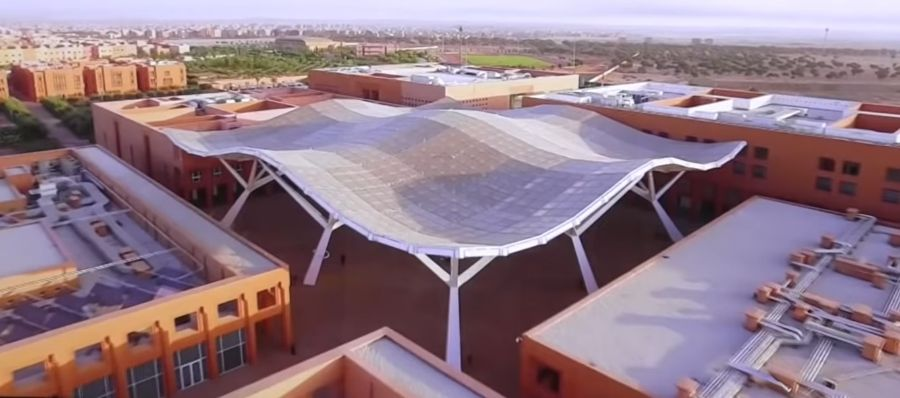
\includegraphics[width=0.82\textwidth]{figures/um6p_campus.jpg}
\caption{Le campus principal de l'UM6P à Benguérir, au sein de la Ville Verte
Mohammed~VI, reconnaissable à sa canopée centrale. \emph{(Source~: Le360,
Wikimedia Commons, licence CC~BY~3.0.)}}
\label{fig:campus}
\end{figure}

L'université s'organise autour de plusieurs écoles et centres de recherche
couvrant un large spectre disciplinaire~: sciences et ingénierie, sciences des
matériaux, agriculture et sécurité alimentaire, sciences économiques et sociales,
énergie, et, de façon transverse, sciences des données et intelligence
artificielle. Cette structuration vise explicitement à décloisonner la recherche
fondamentale, l'expérimentation et l'application industrielle. L'intelligence
artificielle y occupe une place stratégique, à la fois comme domaine de recherche
à part entière et comme levier transversal au service des autres disciplines~;
c'est dans cette dynamique que s'inscrit le centre AI Movement.

\begin{figure}[ht]
\centering

\includegraphics[height=1.3cm]{figures/um6p-aim.png}
\caption{Logos institutionnels de l'UM6P, du centre AI Movement et de l'UNESCO,
sous l'égide de laquelle le centre a été établi.}
\label{fig:logos}
\end{figure}

\subsection{Le centre AI Movement}

Le Centre International d'Intelligence Artificielle du Maroc, connu sous le nom
d'\emph{AI Movement}, constitue un centre d'excellence consacré à l'intelligence
artificielle et aux sciences des données au sein de l'écosystème de l'UM6P,
établi sous l'égide de l'UNESCO. Sa création répond à une volonté de développer
une capacité nationale et africaine en matière d'intelligence artificielle, tout
en favorisant l'ouverture du Maroc sur les réseaux scientifiques et
technologiques internationaux.

AI Movement se positionne comme un pôle dédié à la recherche, à l'innovation et
à la transformation par l'intelligence artificielle. Sa vocation ne se limite
pas au développement de modèles ou d'outils~: le centre cherche également à
favoriser l'émergence d'un écosystème réunissant chercheurs, étudiants,
industriels, institutions publiques et partenaires internationaux. Le projet a
notamment été porté par la Professeure Amal El Fallah Seghrouchni, spécialiste
de l'intelligence artificielle distribuée et des systèmes multi-agents, qui
assure la direction du centre. Sous son impulsion, AI Movement développe des
activités combinant recherche scientifique, formation, innovation technologique,
transfert industriel et réflexion sur les impacts de l'intelligence artificielle.

Le centre conduit des travaux dans plusieurs domaines complémentaires~: la vision
par ordinateur, le traitement automatique du langage naturel, l'apprentissage
automatique et profond, les systèmes multi-agents et l'IA incarnée. Le travail
présenté dans ce rapport se situe précisément à l'intersection des deux premiers
axes~: la \emph{génération de mouvement humain tridimensionnel à partir de
descriptions en langage naturel}, avec un accent mis sur les langues autres que
l'anglais.

\subsection{L'environnement de calcul}

Le développement de travaux de recherche en intelligence artificielle, en
particulier l'entraînement de modèles d'apprentissage profond, nécessite des
capacités de calcul importantes. L'écosystème de l'UM6P dispose à ce titre du
supercalculateur \emph{Toubkal}, infrastructure de calcul haute performance
(\emph{High-Performance Computing}, HPC) hébergée à Benguérir et nommée d'après
le point culminant du Maroc dans le Haut Atlas (figure~\ref{fig:toubkal}). Son
déploiement constitue une étape importante dans le développement des capacités
nationales et africaines de calcul intensif~; il illustre la convergence
croissante entre le HPC et l'intelligence artificielle, les architectures modernes
d'apprentissage profond reposant largement sur des accélérateurs matériels, en
particulier des processeurs graphiques (GPU) permettant d'exécuter efficacement un
grand nombre d'opérations matricielles en parallèle.

\begin{figure}[ht]
\centering
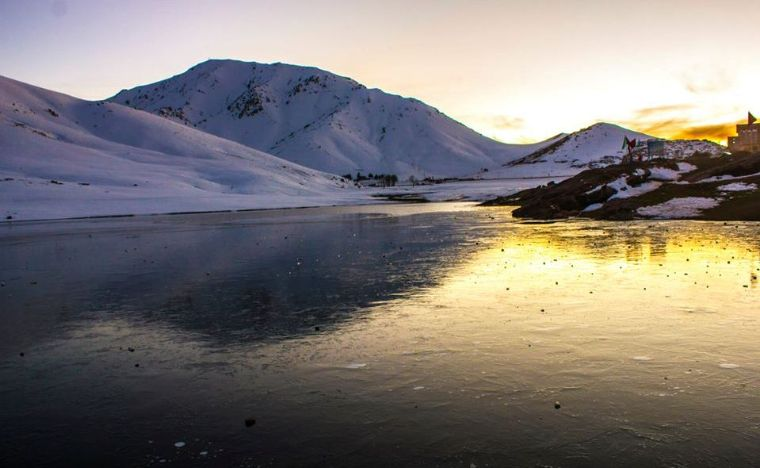
\includegraphics[width=0.74\textwidth]{figures/toubkal_mountain.jpg}
\caption{Le mont Toubkal (Haut Atlas), point culminant de l'Afrique du Nord, dont
le supercalculateur de l'UM6P tire son nom. \emph{(Source~: Yasminaou01,
Wikimedia Commons, licence CC~BY-SA~4.0.)}}
\label{fig:toubkal}
\end{figure}

Il convient de distinguer le \emph{centre} AI Movement de l'\emph{infrastructure}
Toubkal~: cette dernière est une ressource de calcul mutualisée de l'UM6P,
susceptible de soutenir des travaux de recherche très variés, et non un équipement
propre au centre. Elle n'en reste pas moins emblématique de l'ambition de doter
l'écosystème marocain et africain de moyens de calcul à la hauteur des besoins de
l'apprentissage profond moderne.

Le stage s'est déroulé sur une durée de \textbf{dix semaines}. Les expériences
décrites dans ce rapport ont été menées sur une station de
travail équipée d'un GPU \textbf{NVIDIA RTX~5090} (32~Go de mémoire), partagée au
sein de l'équipe. Si cette ressource est modeste au regard d'une grappe de calcul
complète, elle s'est révélée suffisante pour une démarche de recherche fondée sur
des \emph{expériences contrôlées} de petite à moyenne échelle, où la rigueur
méthodologique prime sur le volume brut de calcul.

\subsection{Missions et domaines d'expertise}

La mission d'AI Movement dépasse le cadre strict de la recherche académique. Le
centre vise à structurer un écosystème capable de réunir les compétences
nationales et internationales en intelligence artificielle, notamment par
l'attraction d'experts, la création de partenariats scientifiques et le
développement de collaborations entre chercheurs marocains et étrangers. Ses
missions s'articulent autour de plusieurs axes~:

\begin{itemize}[leftmargin=*]
\item \textbf{Recherche scientifique et développement technologique}~: associer
recherche théorique, recherche appliquée, développement technologique, innovation
et transfert industriel, en rapprochant les laboratoires de recherche des
problématiques concrètes rencontrées par les acteurs économiques et sociaux.
\item \textbf{Formation et développement des compétences}~: favoriser
l'appropriation des technologies d'IA par différentes catégories de public, des
étudiants et jeunes chercheurs jusqu'aux professionnels, à travers des activités
de formation, d'encadrement scientifique, de séminaires et de conférences.
\item \textbf{Transfert technologique et entrepreneuriat}~: transformer les
résultats scientifiques en technologies et produits à forte valeur ajoutée et
encourager l'entrepreneuriat technologique.
\item \textbf{IA responsable et éthique}~: porter une attention particulière à la
transparence, à l'équité, à la protection des données, à la robustesse et à
l'explicabilité des modèles. Cette dimension revêt une importance particulière
dans le contexte africain, où les modèles entraînés majoritairement sur des
données provenant d'autres régions du monde peuvent présenter des performances
variables lorsqu'ils sont appliqués à des populations, des langues ou des
contextes culturels différents.
\end{itemize}

Ce dernier point, l'inclusion linguistique et culturelle, rejoint
directement la motivation du présent projet. L'ambition africaine et
internationale du centre, qui cherche à contribuer à un écosystème de
compétences dépassant le cadre strictement national, trouve un prolongement
naturel dans l'étude de modèles capables de traiter des descriptions de
mouvement dans plusieurs langues, et non uniquement en anglais.

\paragraph{Diversité des axes de recherche.} Les travaux menés au sein de
l'écosystème AI Movement couvrent un éventail large~: apprentissage automatique et
profond, vision par ordinateur, traitement automatique du langage naturel,
systèmes multi-agents, agents intelligents, IA hybride, systèmes autonomes et IA
explicable. Cette diversité permet d'aborder des problématiques nécessitant le
traitement de données hétérogènes et favorise les interactions entre disciplines.
Le projet présenté ici, à la croisée de la vision et du langage, illustre
précisément cette transversalité.

\paragraph{IA hybride et systèmes intelligents.} Une caractéristique de l'approche
défendue par le centre réside dans la complémentarité entre différents paradigmes.
L'IA hybride cherche à associer, selon les besoins, des approches fondées sur
l'apprentissage et des approches symboliques ou à base de connaissances, ouvrant la
voie à des systèmes plus interprétables, plus adaptables et mieux intégrés à leur
environnement. Les systèmes multi-agents, historiquement liés aux travaux de la
direction du centre, en sont un exemple~: plusieurs agents autonomes y perçoivent,
communiquent, coopèrent ou négocient afin d'atteindre des objectifs individuels ou
collectifs.

\paragraph{Formation et transfert.} Le centre participe à des activités de
formation, d'encadrement scientifique, de séminaires et de conférences, et accorde
une attention à la sensibilisation aux transformations induites par l'IA. Il
cherche aussi à transformer les résultats de la recherche en technologies et
produits à forte valeur ajoutée, en développant des relations étroites avec le
monde industriel et en encourageant l'entrepreneuriat technologique. Les domaines
d'application visés incluent l'énergie, l'industrie, la santé, l'agriculture, la
finance et les services numériques.

\subsection{Une dimension africaine, responsable et inclusive}

L'une des spécificités d'AI Movement réside dans son ambition de contribuer au
développement de l'intelligence artificielle à l'échelle africaine. Le centre ne
se limite pas à une mission nationale~: il cherche à participer à la constitution
d'un écosystème continental de recherche, de formation et d'innovation. Cette
ambition s'accompagne d'une attention soutenue à l'\emph{IA responsable}~:
transparence, équité, protection des données et, surtout pour ce qui nous concerne,
\emph{inclusion}.

Les systèmes d'intelligence artificielle reproduisent et amplifient les biais
présents dans leurs données d'entraînement. Un modèle de génération de mouvement
entraîné exclusivement sur des légendes anglaises encode implicitement une
conception anglophone de la description du geste~; appliqué à des utilisateurs
s'exprimant dans d'autres langues, il peut se révéler moins performant, voire
inutilisable. Étudier \emph{si} et \emph{comment} de tels modèles peuvent devenir
multilingues n'est donc pas qu'un exercice technique~: c'est une contribution
directe à l'objectif d'inclusion porté par le centre. C'est dans cette double
perspective, scientifique et sociétale, que s'inscrit le présent projet.

\section{Contexte du projet et problématique}

\subsection{L'essor de la génération de mouvement à partir de texte}

La génération de mouvement humain à partir de texte s'inscrit dans l'essor plus
large des modèles \emph{multimodaux}, capables de mettre en correspondance des
modalités de nature différente, ici le langage et le mouvement
tridimensionnel. Formellement, il s'agit, à partir d'une description textuelle
$c$, de produire une séquence de poses $x = (x_1,\dots,x_T)$ où chaque $x_t$
décrit la configuration du corps à l'instant $t$. La figure~\ref{fig:t2m}
illustre schématiquement cette tâche.

\begin{figure}[ht]
\centering
\begin{tikzpicture}[font=\small,
  node distance=6mm,
  txt/.style={draw=accent,fill=accent!8,rounded corners=3pt,minimum height=12mm,
    align=center,text width=3.2cm},
  mod/.style={draw=bleu,fill=bleutres,rounded corners=3pt,minimum height=12mm,
    align=center,text width=3.0cm},
  outbox/.style={draw=grisligne,fill=grisclair,rounded corners=3pt,minimum height=12mm,
    align=center,text width=3.6cm},
  ar/.style={-{Latex[length=2.4mm]},thick,bleu}]
\node[txt] (c) {\textbf{Texte}\\[1pt]\emph{«~une personne\\marche puis s'assoit~»}};
\node[mod,right=8mm of c] (m) {\textbf{Modèle}\\génératif\\conditionnel};
\node[outbox,right=8mm of m] (x) {\textbf{Séquence de poses 3D}\\$x_1,\dots,x_T$};
\draw[ar] (c)--(m); \draw[ar] (m)--(x);
\end{tikzpicture}
\caption{La tâche de génération texte$\rightarrow$mouvement~: un modèle
conditionnel transforme une description en langage naturel en une séquence de
poses corporelles tridimensionnelles.}
\label{fig:t2m}
\end{figure}

Trois familles de modèles encadrent le travail présenté ici.
\emph{MotionCLIP}~\cite{tevet2022motionclip} est un autoencodeur transformeur qui
aligne un unique latent de mouvement sur l'espace d'embedding figé de CLIP~; c'est
un générateur relativement faible, mais d'une simplicité et d'une transparence
inhabituelles, ce qui en fait un modèle de base idéal pour une étude contrôlée.
\emph{MDM}~\cite{tevet2023mdm} est un modèle de diffusion opérant directement sur
la séquence de mouvement, et \emph{MoMask}~\cite{guo2024momask} est un
transformeur masqué à quantification vectorielle résiduelle qui produit une
\emph{séquence de tokens discrets}. MDM et MoMask sont des générateurs nettement
plus puissants~; la conception de MoMask en séquence de tokens est précisément
l'architecture vers laquelle pointe l'argument final de ce rapport
(chapitre~\ref{ch:discussion}).

\begin{encadre}
\textbf{Un repère à garder à l'esprit.} Le FID publié sur HumanML3D pour les
modèles performants se situe dans la plage $0{,}05$--$0{,}5$~\cite{guo2024momask}.
Tous les FID rapportés dans ce travail sont un à deux ordres de grandeur plus
élevés. MotionCLIP est un générateur \emph{faible}, et les comparaisons menées ici
sont \emph{relatives}, et non absolues.
\end{encadre}

\subsection{État de l'art de la génération texte \texorpdfstring{$\rightarrow$}{vers} mouvement}
\label{sub:etat-art}

La génération de mouvement à partir de texte a connu trois grandes familles
d'approches, qu'il est utile de situer pour comprendre le positionnement de ce
travail.

\paragraph{Approches par espace latent aligné (MotionCLIP).}
\textbf{MotionCLIP}~\cite{tevet2022motionclip} aligne un latent de mouvement sur
l'espace d'embedding figé de CLIP~\cite{radford2021clip}. L'idée séduisante est
d'hériter « gratuitement » de la richesse sémantique de CLIP~: comme le texte et
l'image y sont déjà alignés, aligner le mouvement sur le texte revient à l'ancrer
dans un espace sémantique vaste. En contrepartie, MotionCLIP est un générateur
faible, car il comprime tout un clip en un unique vecteur et s'appuie sur une
simple similarité cosinus. C'est précisément cette simplicité qui en fait un banc
d'essai idéal pour une étude contrôlée des mécanismes d'alignement et de
régularisation.

\paragraph{Approches par diffusion (MDM).}
\textbf{MDM}~\cite{tevet2023mdm} applique un modèle de diffusion directement sur la
séquence de poses~: un processus apprend à débruiter progressivement un mouvement
initialement aléatoire, conditionné par le texte. Cette approche produit des
mouvements nettement plus réalistes et diversifiés, au prix d'un échantillonnage
itératif coûteux. Elle démontre que conserver la \emph{dimension temporelle}
(plutôt que de la comprimer) est déterminant pour la qualité.

\paragraph{Approches par tokens discrets (MoMask).}
\textbf{MoMask}~\cite{guo2024momask} représente un mouvement comme une
\emph{séquence de tokens discrets} obtenus par quantification vectorielle
résiduelle (RVQ), qu'un transformeur masqué génère ensuite de façon itérative.
C'est l'état de l'art en qualité de génération. Son architecture en séquence de
latents discrets est exactement celle vers laquelle pointe la proposition
prospective de ce rapport (chapitre~\ref{ch:discussion})~: elle contourne
structurellement les trois défaillances que nous mettons en évidence sur le latent
unique.

\paragraph{Le banc d'essai HumanML3D et ses extensions.}
L'ensemble de ces modèles est évalué sur HumanML3D~\cite{guo2022humanml3d}, devenu
le standard de fait. Les travaux récents en multilinguisme, notamment
\textbf{BiHumanML3D}~\cite{weng2026bihumanml3d}, proposent une ré-annotation
bilingue de HumanML3D assortie d'un module d'alignement inter-lingue projetant le
texte non anglais dans l'espace de mouvement entraîné en anglais. L'hypothèse
communément admise y est que le signal multilingue est, au pire, \emph{neutre} pour
la représentation du mouvement. C'est cette hypothèse que le présent travail
soumet à un test contrôlé.

Le tableau~\ref{tab:approches} résume le positionnement de ces familles selon trois
axes~: la nature de la représentation du mouvement, le type de conditionnement
textuel et la qualité de génération.

\begin{table}[ht]
\centering
\caption{Positionnement comparatif des principales familles de génération
texte$\rightarrow$mouvement.}
\label{tab:approches}
\small
\begin{tabular}{@{}lp{3.2cm}p{3.0cm}p{3.0cm}@{}}
\toprule
Modèle & Représentation & Conditionnement & Génération \\
\midrule
MotionCLIP & latent unique continu & CLIP (cosinus) & faible \\
T2M~\cite{guo2022humanml3d} & latent variationnel & texte + VAE & moyenne \\
MDM & séquence continue & diffusion & forte \\
MoMask & séquence de tokens (RVQ) & transformeur masqué & état de l'art \\
\textbf{Ce travail} & latent unique + multilingue & M-CLIP (cosinus/CE) & faible (étude contrôlée) \\
\bottomrule
\end{tabular}
\end{table}

On observe une corrélation nette~: les approches qui \emph{préservent la dimension
temporelle} (MDM, MoMask) génèrent nettement mieux que celles qui la
\emph{compriment} en un point (MotionCLIP). Ce constat, dressé ici au niveau de
l'état de l'art, sera retrouvé de l'intérieur par l'analyse expérimentale~: c'est la
compression en un latent unique qui limite MotionCLIP, et non le conditionnement
textuel en lui-même.

\subsection{Le multilinguisme en traitement automatique du langage}
\label{sub:nlp-multi}

Le multilinguisme n'est pas propre au mouvement~: il est étudié depuis longtemps en
traitement automatique du langage. Deux constats issus de ce domaine éclairent
directement notre question. \emph{D'une part}, les modèles massivement multilingues
comme XLM-R~\cite{conneau2020xlmr} montrent un \emph{transfert inter-lingue}
remarquable~: un modèle affiné sur une langue fonctionne souvent, sans données
supplémentaires, sur des langues qu'il n'a vues qu'au pré-entraînement. \emph{D'autre
part}, ces mêmes travaux décrivent une \emph{malédiction du multilinguisme}~: à
capacité fixe, ajouter des langues finit par dégrader la performance de chacune,
parce que toutes se partagent les mêmes paramètres. Les auteurs de XLM-R observent
ainsi que, au-delà d'un certain nombre de langues, il faut augmenter la taille du
modèle pour maintenir la qualité.

Ces deux phénomènes correspondent exactement aux deux hypothèses de notre étude~:
le transfert inter-lingue rejoint l'hypothèse de la supervision enrichie, et la
malédiction du multilinguisme celle de l'espace partagé appauvri. Notre
contribution est de mesurer lequel domine pour le \emph{mouvement}, sur un modèle
dont la capacité est volontairement fixe. La section~\ref{sec:controlee} montre que
nous observons les deux à la fois~: un transfert réel vers des langues jamais vues,
et une division du budget sur les langues entraînées.

\subsection{Le verrou du multilinguisme}

Comme indiqué en introduction, l'ensemble de cet écosystème s'est développé sur
un corpus exclusivement anglais, HumanML3D~\cite{guo2022humanml3d}. Cette
mono-langue n'est pas qu'une limitation pratique~; elle soulève une question
scientifique précise. On distingue deux hypothèses concurrentes~:

\begin{itemize}[leftmargin=*]
\item \textbf{Hypothèse de la supervision enrichie.} Les langues encodant
différemment la manière, la trajectoire et l'aspect d'un mouvement, un modèle
multilingue pourrait disposer d'un signal \emph{complémentaire} et apprendre une
représentation du mouvement plus riche que son homologue monolingue.
\item \textbf{Hypothèse de l'espace partagé appauvri.} À capacité fixe, les
langues se partagent un budget représentationnel borné~; les ajouter reviendrait
alors à \emph{diviser} ce budget, dégradant la qualité de l'espace latent plutôt
que de l'enrichir.
\end{itemize}

Les travaux récents sur le multilinguisme en génération de mouvement, notamment
le banc d'essai BiHumanML3D~\cite{weng2026bihumanml3d}, supposent le plus souvent
que le signal multilingue est, au pire, neutre pour la représentation du
mouvement sous-jacente. Ce rapport teste cette hypothèse directement, dans des
conditions contrôlées.

\subsection{Question de recherche et positionnement}

La question centrale, déjà énoncée en introduction, peut être reformulée en deux
sous-questions mesurables~:

\begin{enumerate}[leftmargin=*,label=\textbf{RQ\arabic*.}]
\item Des projections de texte entraînées \emph{indépendamment} pour chaque
langue placent-elles plusieurs langues dans un espace latent de mouvement
\emph{commun}~? (Question d'\emph{alignement}.)
\item À capacité et à budget de calcul appariés, le conditionnement multilingue
\emph{aide-t-il ou nuit-il} à la représentation du mouvement, mesurée sur un jeu
de test commun~? (Question de \emph{qualité}.)
\end{enumerate}

Répondre à ces questions suppose une comparaison qui, à notre connaissance,
n'avait pas été menée~: anglais seul contre multilingue, \emph{appariés en
capacité de modèle et en nombre de pas de gradient}, évalués sur un même jeu de
test afin que les chiffres soient directement comparables. Elle suppose aussi de
\emph{localiser} l'origine de toute dégradation, dans l'encodeur de texte
figé, ou dans le latent de mouvement entraîné. Comme on le verra, cette seconde
mesure, effectuée sans précaution méthodologique, conduit à une conclusion
erronée~: une part importante de ce rapport consiste précisément à construire la
bonne mesure d'alignement.

% =====================================================================
% CHAPITRE 2 : CADRE THEORIQUE
% =====================================================================
\chapter{Cadre théorique et fondements mathématiques}
\label{ch:theorie}

Ce chapitre rassemble les fondements théoriques nécessaires à la compréhension
du travail. Après quelques rappels d'apprentissage profond (section~\ref{sec:dl}),
il décrit la manière dont un mouvement humain est représenté numériquement
(section~\ref{sec:motion}), introduit l'architecture Transformer et le mécanisme
d'attention qui sous-tendent le modèle (section~\ref{sec:transfo}), puis développe
la théorie des autoencodeurs variationnels (section~\ref{sec:vae}) et de la
quantification vectorielle (section~\ref{sec:vq}), celle de l'apprentissage
contrastif et de l'alignement vision--langage (section~\ref{sec:contrastif}), les
représentations multilingues (section~\ref{sec:multiling}) et l'apprentissage par
transfert (section~\ref{sec:transfert}). Il présente ensuite les métriques
d'évaluation génératives (section~\ref{sec:metriques}) et se clôt par une analyse
mathématique du goulot d'étranglement latent (section~\ref{sec:goulot}), qui
fournit l'armature théorique de plusieurs résultats du chapitre~\ref{ch:resultats}.

\section{Rappels d'apprentissage profond}
\label{sec:dl}

Avant d'aborder les architectures spécifiques, on rappelle brièvement les notions
d'apprentissage profond mobilisées dans tout le rapport.

\subsection{Du perceptron au réseau multicouche}

L'unité de base est le \emph{neurone artificiel}, qui calcule une combinaison
linéaire de ses entrées suivie d'une non-linéarité~: $y = \varphi(w^\top x + b)$, où
$w$ est un vecteur de poids, $b$ un biais et $\varphi$ une fonction d'activation. Un
\emph{réseau multicouche} (MLP) empile de telles unités en couches successives, de
sorte que la sortie d'une couche alimente la suivante. La fonction d'activation
employée ici est la \textbf{GELU}~\cite{hendrycks2016gelu} (\emph{Gaussian Error Linear Unit}),
$\varphi(x) = x\,\Phi(x)$ où $\Phi$ est la fonction de répartition de la loi
normale~; elle est lisse et différentiable partout, ce qui facilite l'optimisation.
Le théorème d'approximation universelle garantit qu'un MLP suffisamment large peut
approcher n'importe quelle fonction continue~; en pratique, c'est la \emph{profondeur}
et les \emph{structures spécialisées} (attention, convolutions) qui rendent
l'apprentissage efficace.

\subsection{Apprentissage par descente de gradient}

L'entraînement consiste à minimiser une fonction de coût $\mathcal{L}(\theta)$ par
rapport aux paramètres $\theta$ du réseau, au moyen de la \emph{descente de gradient
stochastique}~: $\theta \leftarrow \theta - \eta\,\nabla_\theta\mathcal{L}$, où
$\eta$ est le taux d'apprentissage. Le gradient $\nabla_\theta\mathcal{L}$ est
calculé par \emph{rétropropagation}, application de la règle de dérivation en chaîne
qui propage l'erreur de la sortie vers l'entrée, couche par couche. En pratique, on
utilise des optimiseurs adaptatifs (de type Adam~\cite{kingma2015adam}) qui ajustent le pas par paramètre
à partir des moments du gradient, et l'on traite les données par \emph{lots}
(\emph{mini-batches}) pour estimer le gradient de façon efficace~; la taille de lot
(ici~128) influe sur la stabilité et, dans le cas contrastif, sur le nombre de
négatifs disponibles (section~\ref{sec:contrastif}).

\subsection{Généralisation et régularisation}

Un modèle doit \emph{généraliser} au-delà des données d'entraînement. Un modèle
trop flexible \emph{surapprend} (il mémorise le bruit)~; un modèle trop contraint
\emph{sous-apprend}. Plusieurs mécanismes régularisent l'apprentissage~: la
normalisation de couche (stabilisation des activations), les connexions résiduelles
(facilitation du flux de gradient), et, dans le cas d'un VAE, le terme KL qui
régularise l'espace latent (section~\ref{sec:vae}). Un thème récurrent de ce rapport
est que la régularisation \emph{apparente} (par exemple la force du terme KL) peut
être trompeuse~: ce qui gouverne réellement le comportement du modèle est parfois
une autre variable (ici l'échantillonnage, section~\ref{sec:kl}).

\section{Représentation du mouvement humain tridimensionnel}
\label{sec:motion}

\subsection{Du modèle corporel SMPL au squelette}

La génération de mouvement suppose d'abord une représentation numérique du corps
humain. Le modèle de référence est \textbf{SMPL}~\cite{loper2015smpl}
(\emph{Skinned Multi-Person Linear model}), un modèle paramétrique qui décrit le
corps par un petit nombre de paramètres de \emph{forme} (morphologie) et de
\emph{pose} (orientation des articulations). À partir de ces paramètres, SMPL
produit un maillage tridimensionnel complet. Pour la génération de mouvement, on
travaille le plus souvent sur une version simplifiée~: un \emph{squelette} de
quelques dizaines d'articulations reliées par des segments rigides, chaque
articulation étant repérée par ses coordonnées 3D (figure~\ref{fig:skel}).

\begin{figure}[ht]
\centering
\begin{tikzpicture}[font=\footnotesize,
  joint/.style={circle,fill=bleu,inner sep=1.6pt},
  bone/.style={bleu,line width=1.1pt},
  axe/.style={-{Latex[length=1.6mm]},grisfonce}]
% simple skeleton
\coordinate (head) at (0,3.0);
\coordinate (neck) at (0,2.5);
\coordinate (sho_l) at (-0.7,2.4);
\coordinate (sho_r) at (0.7,2.4);
\coordinate (elb_l) at (-1.05,1.7);
\coordinate (elb_r) at (1.05,1.7);
\coordinate (han_l) at (-1.2,1.0);
\coordinate (han_r) at (1.2,1.0);
\coordinate (pel)   at (0,1.4);
\coordinate (hip_l) at (-0.4,1.35);
\coordinate (hip_r) at (0.4,1.35);
\coordinate (kne_l) at (-0.5,0.6);
\coordinate (kne_r) at (0.5,0.6);
\coordinate (foo_l) at (-0.55,0.0);
\coordinate (foo_r) at (0.55,0.0);
\draw[bone] (neck)--(head);
\draw[bone] (sho_l)--(neck)--(sho_r);
\draw[bone] (sho_l)--(elb_l)--(han_l);
\draw[bone] (sho_r)--(elb_r)--(han_r);
\draw[bone] (neck)--(pel);
\draw[bone] (hip_l)--(pel)--(hip_r);
\draw[bone] (hip_l)--(kne_l)--(foo_l);
\draw[bone] (hip_r)--(kne_r)--(foo_r);
\foreach \p in {head,neck,sho_l,sho_r,elb_l,elb_r,han_l,han_r,pel,hip_l,hip_r,kne_l,kne_r,foo_l,foo_r}
  \node[joint] at (\p) {};
% root axes
\draw[axe] (pel)--++(0.9,0) node[right]{$x$};
\draw[axe] (pel)--++(0,0.9) node[above]{$y$};
\node[fill=bleutres,draw=grisligne,rounded corners=2pt,inner sep=2pt] at (0,-0.45) {racine (\emph{root})};
\end{tikzpicture}
\caption{Représentation squelettique du corps humain~: chaque articulation est
un point 3D, relié à ses voisines par des segments. La racine (bassin) porte le
repère global par rapport auquel les positions locales sont exprimées.}
\label{fig:skel}
\end{figure}

\subsection{La représentation HumanML3D à 263 dimensions}

Le jeu de données utilisé est \textbf{HumanML3D}~\cite{guo2022humanml3d}, qui
apparie des mouvements humains 3D à des légendes en anglais. Chaque mouvement est
une séquence d'images (\emph{frames}), et chaque image est encodée par un vecteur
de pose \emph{redondant} de \textbf{263 dimensions}, dérivé du modèle SMPL. Cette
redondance est volontaire~: elle fournit au réseau plusieurs vues cohérentes de
la même pose, ce qui facilite l'apprentissage. La décomposition des 263
composantes est la suivante~:

\begin{center}
\setlength{\tabcolsep}{10pt}
\begin{tabular}{@{}lcp{6.6cm}@{}}
\toprule
\textbf{Bloc} & \textbf{Dim.} & \textbf{Contenu} \\
\midrule
Racine & 4 & vitesse angulaire, vitesses linéaires $x,z$, hauteur $y$ \\
Positions locales & 63 & coordonnées 3D de 21 articulations ($21\times3$) \\
Rotations locales & 126 & rotations \emph{continues} 6D de 21 articulations ($21\times6$) \\
Vitesses locales & 66 & vitesses 3D de 22 articulations ($22\times3$) \\
Contacts au sol & 4 & indicateurs binaires de contact des pieds \\
\midrule
\textbf{Total} & \textbf{263} & \\
\bottomrule
\end{tabular}
\end{center}

Ce travail manipule des clips de \textbf{longueur fixe de 60 images}~; un clip est
donc un tenseur de $60\times263 = 15\,780$ nombres. Après filtrage, le corpus
fournit \textbf{22\,326} clips d'entraînement (966 écartés car trop courts, 92 car
trop longs) et \textbf{1\,400} clips de validation. Cette contrainte de longueur
fixe, combinée à la compression en un latent unique étudiée plus loin, est au
cœur des phénomènes analysés dans ce rapport.

\subsection{Le modèle paramétrique SMPL}
\label{sub:smpl}

Le modèle SMPL~\cite{loper2015smpl} formalise le corps humain comme une fonction
différentiable $M(\beta,\theta)$ qui produit un maillage de $N=6890$ sommets à
partir de deux groupes de paramètres~: un vecteur de \emph{forme}
$\beta\in\R^{10}$ (les dix premières composantes principales de la morphologie,
apprises sur des milliers de scans 3D) et un vecteur de \emph{pose}
$\theta\in\R^{3\times24}$ (les rotations axe-angle des 24 articulations du
squelette). Le maillage se calcule en trois étapes~:
\begin{equation}
M(\beta,\theta) = W\big(T_P(\beta,\theta),\, J(\beta),\, \theta,\, \mathcal{W}\big),
\quad
T_P(\beta,\theta) = \bar{T} + B_S(\beta) + B_P(\theta),
\label{eq:smpl}
\end{equation}
où $\bar{T}$ est un gabarit moyen, $B_S(\beta)$ et $B_P(\theta)$ sont des
\emph{blend shapes} linéaires corrigeant respectivement la morphologie et les
déformations dépendant de la pose, $J(\beta)$ régresse la position des
articulations, et $W(\cdot)$ est l'opérateur de \emph{linear blend skinning} qui
déforme le gabarit selon les rotations $\theta$ et les poids d'attache
$\mathcal{W}$. La différentiabilité de l'équation~\eqref{eq:smpl} est essentielle~:
elle permet de rétropropager un gradient depuis une perte définie sur les
articulations jusqu'aux paramètres. Pour la génération de mouvement, on ne
manipule pas le maillage complet mais une abstraction squelettique (les positions
et rotations articulaires), bien plus légère et suffisante pour décrire le geste.

\subsection{Arbre cinématique et cinématique directe}
\label{sub:fk}

Le squelette est organisé en \emph{arbre cinématique}~: chaque articulation $j$
possède un parent $\pi(j)$, la racine (le bassin) n'en ayant pas. La position d'une
articulation se déduit de celle de son parent, de la rotation locale et de la
longueur du segment qui les relie. En notant $R_j$ la rotation locale de
l'articulation $j$ et $o_j$ le décalage fixe (l'os) vers son parent, la
transformation globale se calcule récursivement depuis la racine~:
\begin{equation}
G_j = G_{\pi(j)}\begin{pmatrix} R_j & o_j\\ 0 & 1\end{pmatrix},\qquad
p_j = G_j\begin{pmatrix}0\\0\\0\\1\end{pmatrix},
\label{eq:fk}
\end{equation}
où $G_j$ est une matrice homogène $4\times4$ et $p_j$ la position globale. C'est la
\emph{cinématique directe}. Cette structure explique une propriété du mouvement
importante pour la suite~: une petite erreur de rotation sur une articulation
proche de la racine (hanche, épaule) se \emph{propage} à toute la chaîne qui en
dépend (genou, cheville~; coude, poignet). C'est l'une des raisons pour lesquelles
HumanML3D fournit à la fois des positions et des rotations~: la redondance limite
l'accumulation d'erreurs le long de l'arbre.

\subsection{Rotations continues et normalisation des données}
\label{sub:rotations}

Un détail technique important de la représentation HumanML3D concerne le codage
des \emph{rotations}. Les paramétrisations classiques (angles d'Euler,
quaternions) souffrent de discontinuités ou d'ambiguïtés
($q$ et $-q$ codent la même rotation) qui nuisent à l'apprentissage par réseau de
neurones. HumanML3D adopte donc la représentation \emph{continue à 6 dimensions}~\cite{zhou2019continuity}~:
une rotation $R\in SO(3)$ est codée par ses deux premières colonnes
$(\mathbf{a}_1,\mathbf{a}_2)\in\R^6$, la troisième étant reconstruite par produit
vectoriel après orthonormalisation de Gram--Schmidt~:
\begin{equation}
\mathbf{b}_1 = \frac{\mathbf{a}_1}{\lVert\mathbf{a}_1\rVert},\quad
\mathbf{b}_2 = \frac{\mathbf{a}_2 - (\mathbf{b}_1\!\cdot\!\mathbf{a}_2)\mathbf{b}_1}
{\lVert\mathbf{a}_2 - (\mathbf{b}_1\!\cdot\!\mathbf{a}_2)\mathbf{b}_1\rVert},\quad
\mathbf{b}_3 = \mathbf{b}_1\times\mathbf{b}_2 .
\end{equation}
Cette application $\R^6\to SO(3)$ est \emph{continue et surjective}, ce qui élimine
les discontinuités et explique le bloc de 126 dimensions ($21\times6$) de la
représentation. Enfin, chaque composante du vecteur de 263 dimensions est
\emph{standardisée} (retrait de la moyenne et division par l'écart-type calculés
sur le corpus d'entraînement) avant d'entrer dans le réseau~; c'est pourquoi une
erreur de reconstruction $\rc$ de l'ordre de $0{,}08$ correspond à une
reconstruction visuellement fidèle, tandis qu'une valeur de $0{,}5$ traduit un
effondrement (section~\ref{sec:kl}).

\section{Le Transformer et le mécanisme d'attention}
\label{sec:transfo}

L'architecture retenue par MotionCLIP est un \textbf{Transformer}, introduit par
Vaswani \emph{et al.}~\cite{vaswani2017attention}. Contrairement aux réseaux
récurrents, le Transformer traite une séquence entière en parallèle et met en
relation toutes ses positions grâce au mécanisme d'\emph{auto-attention}.

\subsection{Les modèles de séquence avant le Transformer}

Historiquement, les séquences étaient traitées par des \emph{réseaux récurrents}
(RNN) et leurs variantes à portes (LSTM, GRU), qui maintiennent un état caché mis à
jour image après image. Ces modèles souffrent de deux limites~: le traitement est
intrinsèquement \emph{séquentiel} (l'état à l'instant $t$ dépend de l'instant
$t-1$), ce qui empêche la parallélisation~; et les dépendances à longue portée
s'estompent (problème du gradient qui s'évanouit), car l'information doit transiter
par tous les états intermédiaires. Les réseaux convolutifs atténuent la première
limite (traitement parallèle) mais ne relient que des positions \emph{voisines} par
couche. Le Transformer résout les deux à la fois~: toute paire de positions est
reliée en une seule opération (chemin de longueur $\mathcal{O}(1)$), et l'ensemble
de la séquence est traité en parallèle (tableau~\ref{tab:complexite}). C'est cette
capacité à modéliser des dépendances globales qui en a fait l'architecture
dominante, y compris pour le mouvement.

\subsection{Le mécanisme d'attention}

Soit une séquence de $N$ vecteurs d'entrée rassemblés dans une matrice
$X\in\R^{N\times d}$. Trois projections linéaires produisent les
\emph{requêtes}, \emph{clés} et \emph{valeurs}~:
\begin{equation}
Q = XW_Q,\qquad K = XW_K,\qquad V = XW_V,
\end{equation}
avec $W_Q,W_K,W_V\in\R^{d\times d_k}$. L'attention à produit scalaire normalisé
calcule alors
\begin{equation}
\mathrm{Attention}(Q,K,V) = \mathrm{softmax}\!\left(\frac{QK^{\top}}{\sqrt{d_k}}\right)V .
\label{eq:attention}
\end{equation}
Le produit $QK^{\top}\in\R^{N\times N}$ mesure la similarité entre chaque paire de
positions~; la normalisation par $\sqrt{d_k}$ stabilise les gradients, et le
$\mathrm{softmax}$ transforme chaque ligne en une distribution de poids. Chaque
position de sortie est ainsi une moyenne pondérée des valeurs de \emph{toutes} les
positions d'entrée (figure~\ref{fig:attn}).

\begin{figure}[ht]
\centering
\begin{tikzpicture}[font=\footnotesize,
  m/.style={draw=bleu,fill=bleutres,minimum width=7mm,minimum height=7mm},
  lbl/.style={grisfonce},
  ar/.style={-{Latex[length=2mm]},thick,bleu}]
\node[m] (q) at (0,0) {$Q$};
\node[m] (k) at (0,-1.1) {$K$};
\node[m] (v) at (0,-2.2) {$V$};
\node[draw=accent,fill=accent!8,rounded corners=2pt,minimum height=9mm,text width=2.4cm,align=center] (s) at (3.0,-0.55) {$\mathrm{softmax}\!\big(\tfrac{QK^\top}{\sqrt{d_k}}\big)$};
\node[draw=bleu,fill=bleutres,rounded corners=2pt,minimum height=9mm,text width=2.2cm,align=center] (o) at (6.2,-1.1) {sortie\\ pondérée};
\draw[ar] (q.east)--(s.west);
\draw[ar] (k.east)--(s.west);
\draw[ar] (s.east)--(o.west);
\draw[ar] (v.east)-- ++(4.1,0) |- (o.west);
\end{tikzpicture}
\caption{Le mécanisme d'attention de l'équation~\eqref{eq:attention}~: les
similarités requête--clé, normalisées par un $\mathrm{softmax}$, pondèrent les
valeurs pour produire chaque vecteur de sortie.}
\label{fig:attn}
\end{figure}

\subsection{Normalisation par \texorpdfstring{$\sqrt{d_k}$}{sqrt(dk)} et propriétés du softmax}

Le facteur de normalisation $1/\sqrt{d_k}$ de l'équation~\eqref{eq:attention}
n'est pas cosmétique. Si les composantes de $q$ et $k$ sont des variables
aléatoires indépendantes de moyenne nulle et de variance unité, leur produit
scalaire $q\cdot k = \sum_{i=1}^{d_k} q_i k_i$ a une variance de $d_k$. Sans
normalisation, les logits passés au $\mathrm{softmax}$ croissent donc comme
$\sqrt{d_k}$~; pour $d_k$ grand, le $\mathrm{softmax}$ sature (une entrée domine,
les autres s'annulent) et son gradient devient négligeable. Diviser par
$\sqrt{d_k}$ ramène la variance des logits à l'unité et préserve des gradients
exploitables. Rappelons que le $\mathrm{softmax}$ transforme un vecteur de logits
$s$ en une distribution $\mathrm{softmax}(s)_i = e^{s_i}/\sum_j e^{s_j}$, dont la
jacobienne $\partial\,\mathrm{softmax}(s)_i/\partial s_j = p_i(\delta_{ij} - p_j)$
tend vers zéro lorsque la distribution $p$ est saturée~: d'où l'importance de la
normalisation.

\subsection{Attention multi-têtes}

En pratique, on emploie l'\emph{attention multi-têtes}~: au lieu d'une unique
fonction d'attention, on en calcule $h$ en parallèle, chacune sur une projection
distincte de dimension $d_k = d/h$~:
\begin{equation}
\mathrm{MultiHead}(X) = \big[\,\mathrm{t\hat{e}te}_1;\dots;\mathrm{t\hat{e}te}_h\,\big]\,W_O,
\qquad
\mathrm{t\hat{e}te}_i = \mathrm{Attention}(XW_Q^{(i)}, XW_K^{(i)}, XW_V^{(i)}),
\end{equation}
où $[\,\cdot\,;\,\cdot\,]$ désigne la concaténation et $W_O\in\R^{d\times d}$ une
projection de sortie. Chaque tête peut ainsi se spécialiser dans un type de
dépendance (proximité temporelle, symétrie gauche/droite du corps, coordination de
membres), et leur concaténation combine ces vues.

\subsection{Encodage de position}

L'opération d'attention étant \emph{invariante par permutation} des positions, un
\emph{encodage de position} est ajouté aux entrées pour réintroduire l'ordre
temporel. L'encodage sinusoïdal d'origine~\cite{vaswani2017attention} s'écrit, pour
la position $t$ et la dimension $2i$ (resp. $2i+1$)~:
\begin{equation}
PE_{(t,2i)} = \sin\!\big(t/10000^{\,2i/d}\big),\qquad
PE_{(t,2i+1)} = \cos\!\big(t/10000^{\,2i/d}\big).
\end{equation}
Ce choix fournit, pour chaque paire de positions, un décalage de phase constant qui
permet au modèle d'exprimer des dépendances relatives et de généraliser à des
longueurs non vues à l'entraînement.

\subsection{Bloc Transformer, encodeur et décodeur}

Un \emph{bloc} Transformer enchaîne une sous-couche d'attention multi-têtes et une
sous-couche \emph{feed-forward} par position (deux transformations linéaires
séparées par une activation GELU), chacune entourée d'une connexion résiduelle et
d'une normalisation de couche (figure~\ref{fig:block})~:
\begin{align}
X' &= \mathrm{LayerNorm}\big(X + \mathrm{MultiHead}(X)\big),\\
X'' &= \mathrm{LayerNorm}\big(X' + \mathrm{FFN}(X')\big),\quad
\mathrm{FFN}(x) = \mathrm{GELU}(xW_1 + b_1)W_2 + b_2 .
\end{align}
Un encodeur empile plusieurs de ces blocs~; un décodeur fait de même en y
ajoutant une sous-couche d'attention croisée vers la sortie de l'encodeur.
MotionCLIP utilise un encodeur--décodeur de \textbf{8~couches} avec activations
GELU.

\begin{figure}[ht]
\centering
\begin{tikzpicture}[font=\footnotesize,
  blk/.style={draw=bleu,fill=bleutres,rounded corners=2pt,minimum width=44mm,
    minimum height=8mm,align=center},
  pl/.style={draw=accent,fill=accent!10,circle,inner sep=0pt,minimum size=5.5mm,
    font=\small},
  nrm/.style={draw=grisligne,fill=grisclair,rounded corners=2pt,minimum width=44mm,
    minimum height=6mm,align=center,font=\scriptsize},
  ar/.style={-{Latex[length=1.8mm]},thick,bleu},
  sk/.style={-{Latex[length=1.6mm]},thick,grisfonce,dashed}]
\node[blk] (in) {entrée $X$ + encodage de position};
\node[blk,above=9mm of in] (mha) {Attention multi-têtes};
\node[pl,above=5mm of mha] (p1) {$+$};
\node[nrm,above=3.5mm of p1] (n1) {LayerNorm};
\node[blk,above=8mm of n1] (ffn) {Feed-Forward (GELU)};
\node[pl,above=5mm of ffn] (p2) {$+$};
\node[nrm,above=3.5mm of p2] (n2) {LayerNorm};
\node[blk,above=8mm of n2] (out) {sortie du bloc};
\draw[ar] (in)--(mha); \draw[ar] (mha)--(p1); \draw[ar] (p1)--(n1);
\draw[ar] (n1)--(ffn); \draw[ar] (ffn)--(p2); \draw[ar] (p2)--(n2);
\draw[ar] (n2)--(out);
% connexions résiduelles : entrée de la sous-couche vers l'addition
\draw[sk] (in.east) -- ++(0.95,0) |- (p1.east);
\draw[sk] (n1.east) -- ++(0.95,0) |- (p2.east);
\node[grisfonce,align=left,font=\scriptsize,right=2mm of p1,xshift=10mm]
  {connexions\\résiduelles};
\end{tikzpicture}
\caption{Structure d'un bloc Transformer~: chaque sous-couche (attention
multi-têtes, puis réseau feed-forward) est suivie d'une addition résiduelle
($+$, l'entrée de la sous-couche est réinjectée) et d'une normalisation de couche.}
\label{fig:block}
\end{figure}

\subsection{Complexité et motivation des latents séquentiels}

Le coût dominant est celui de l'attention~: le produit $QK^{\top}\in\R^{N\times N}$
a une complexité en temps et en mémoire de $\mathcal{O}(N^2 d)$,
\emph{quadratique} en la longueur de séquence $N$ (tableau~\ref{tab:complexite}).
Pour des clips de 60~images, ce coût reste modeste~; il devient en revanche
déterminant pour les séquences longues. Ce fait, conjugué à l'analyse du goulot
latent de la section~\ref{sec:goulot}, motive les architectures à \emph{tokens
discrets} vers lesquelles pointe le chapitre~\ref{ch:discussion}.

\begin{table}[ht]
\centering
\caption{Complexité par couche selon le type de réseau séquentiel ($N$~: longueur
de séquence, $d$~: dimension du modèle).}
\label{tab:complexite}
\small
\begin{tabular}{@{}lccc@{}}
\toprule
Type de couche & Complexité par couche & Opérations séquentielles & Chemin max. \\
\midrule
Récurrente (RNN) & $\mathcal{O}(N d^2)$ & $\mathcal{O}(N)$ & $\mathcal{O}(N)$ \\
Convolutive      & $\mathcal{O}(k N d^2)$ & $\mathcal{O}(1)$ & $\mathcal{O}(\log_k N)$ \\
Auto-attention   & $\mathcal{O}(N^2 d)$ & $\mathcal{O}(1)$ & $\mathcal{O}(1)$ \\
\bottomrule
\end{tabular}
\end{table}

\section{Autoencodeurs et autoencodeurs variationnels}
\label{sec:vae}

\subsection{Autoencodeur déterministe}

Un \textbf{autoencodeur} (AE) est constitué d'un encodeur $E$ qui compresse une
entrée $x$ en un code latent $z = E(x)$, et d'un décodeur $D$ qui reconstruit
$\hat{x} = D(z)$. L'apprentissage minimise une erreur de reconstruction, le plus
souvent quadratique~:
\begin{equation}
\mathcal{L}_{\text{AE}} = \lVert D(E(x)) - x\rVert^2 .
\end{equation}
Dans MotionCLIP, l'encodeur lit un clip de 60~images et, via un jeton de requête
appris, le compresse en un \textbf{unique vecteur latent de dimension~512}~; le
décodeur reconstruit les 60~images à partir de ce seul vecteur. Il s'agit d'une
compression $30\times$ à travers un point unique, fait structurant sur lequel
reposera une grande partie de l'analyse.

\subsection{Autoencodeur variationnel (VAE)}

Un \textbf{autoencodeur variationnel}~\cite{kingma2014vae} remplace le code
ponctuel par une \emph{distribution}. L'encodeur produit les paramètres d'une
gaussienne $q_\phi(z\mid x) = \Ncal(\mu, \sigma^2)$, et le latent est
\emph{échantillonné} à partir de cette distribution. L'objectif est de maximiser
la borne inférieure de la vraisemblance (\emph{Evidence Lower Bound}, ELBO)~:
\begin{equation}
\log p_\theta(x)\;\ge\;\underbrace{\E_{q_\phi(z\mid x)}\big[\log p_\theta(x\mid z)\big]}_{\text{reconstruction}}
\;-\;\underbrace{\KL\!\big(q_\phi(z\mid x)\,\|\,p(z)\big)}_{\text{régularisation}} ,
\label{eq:elbo}
\end{equation}
où $p(z) = \Ncal(0, I)$ est une loi \emph{a priori} unitaire. Le premier terme
pousse le décodeur à bien reconstruire~; le second rapproche la distribution
encodée de la loi a priori, ce qui \emph{lisse} l'espace latent et le rend
génératif. Pour une gaussienne diagonale, la divergence KL admet une forme
close~:
\begin{equation}
\KL\!\big(\Ncal(\mu,\sigma^2)\,\|\,\Ncal(0,I)\big)
= -\tfrac{1}{2}\sum_{i}\big(1 + \log\sigma_i^2 - \mu_i^2 - \sigma_i^2\big).
\label{eq:kl}
\end{equation}

\subsection{Dérivation de la borne ELBO}

La borne de l'équation~\eqref{eq:elbo} n'est pas postulée~: elle découle de
l'introduction d'une distribution d'approximation $q_\phi(z\mid x)$ et de
l'inégalité de Jensen. En partant de la log-vraisemblance marginale et en y
insérant $q_\phi$~:
\begin{align}
\log p_\theta(x)
&= \log\!\int p_\theta(x,z)\,\mathrm{d}z
 = \log\,\E_{q_\phi(z\mid x)}\!\left[\frac{p_\theta(x,z)}{q_\phi(z\mid x)}\right]\\
&\ge \E_{q_\phi(z\mid x)}\!\left[\log\frac{p_\theta(x,z)}{q_\phi(z\mid x)}\right]
 = \underbrace{\E_{q_\phi}\big[\log p_\theta(x\mid z)\big]}_{\text{reconstruction}}
 - \underbrace{\KL\!\big(q_\phi(z\mid x)\,\|\,p(z)\big)}_{\text{régularisation}},
\end{align}
le passage à la deuxième ligne utilisant la concavité du logarithme (Jensen).
L'écart exact entre $\log p_\theta(x)$ et l'ELBO est précisément
$\KL(q_\phi(z\mid x)\,\|\,p_\theta(z\mid x))\ge0$~; maximiser l'ELBO revient donc à
la fois à expliquer les données et à rapprocher la postérieure approchée
$q_\phi$ de la vraie postérieure $p_\theta(z\mid x)$. Dans notre cadre, le terme de
reconstruction est l'erreur quadratique $\rc$ (hypothèse gaussienne sur
$p_\theta(x\mid z)$) et le terme de régularisation est la forme close
\eqref{eq:kl}.

\subsection{L'astuce de reparamétrisation}

L'échantillonnage $z\sim\Ncal(\mu,\sigma^2)$ n'est pas directement
différentiable. L'\emph{astuce de reparamétrisation} contourne ce problème en
écrivant
\begin{equation}
z = \mu + \sigma\odot\varepsilon,\qquad \varepsilon\sim\Ncal(0,I),
\label{eq:reparam}
\end{equation}
où $\odot$ est le produit terme à terme. Le bruit $\varepsilon$ est externe et
indépendant des paramètres~; le gradient peut donc remonter à travers $\mu$ et
$\sigma$ (figure~\ref{fig:vae}). C'est précisément cette étape d'échantillonnage
qui rend l'espace latent lisse et générateur, et c'est aussi, comme le montre
la section~\ref{sec:goulot}, ce qu'un décodeur de mouvement à latent unique ne
peut pas tolérer.

\begin{figure}[ht]
\centering
\begin{tikzpicture}[font=\footnotesize,
  b/.style={draw=grisligne,fill=grisclair,rounded corners=2pt,minimum height=9mm,minimum width=14mm,align=center},
  l/.style={draw=bleu,fill=bleutres,rounded corners=2pt,minimum height=8mm,minimum width=10mm,align=center},
  zbox/.style={draw=bleu,fill=bleutres,rounded corners=2pt,minimum height=9mm,minimum width=30mm,align=center},
  n/.style={draw=accent,fill=accent!8,rounded corners=2pt,minimum height=8mm,minimum width=22mm,align=center},
  ar/.style={-{Latex[length=2mm]},thick,bleu}]
\node[b] (x) {$x$};
\node[b,right=8mm of x] (enc) {Encodeur\\$E_\phi$};
\node[l,above right=5mm and 11mm of enc] (mu) {$\mu$};
\node[l,below right=5mm and 11mm of enc] (sg) {$\sigma$};
\node[zbox,right=30mm of enc] (zz) {$z=\mu+\sigma\odot\varepsilon$};
\node[n,above=8mm of zz] (eps) {$\varepsilon\sim\Ncal(0,I)$};
\node[b,right=10mm of zz] (dec) {Décodeur\\$D_\theta$};
\node[b,right=8mm of dec] (xh) {$\hat x$};
\draw[ar] (x)--(enc);
\draw[ar] (enc)--(mu); \draw[ar] (enc)--(sg);
\draw[ar] (mu)--(zz); \draw[ar] (sg)--(zz);
\draw[ar,accent] (eps)--(zz);
\draw[ar] (zz)--(dec); \draw[ar] (dec)--(xh);
\node[below=1mm of zz,font=\scriptsize\itshape,text=bleu] {reparamétrisation};
\end{tikzpicture}
\caption{Autoencodeur variationnel avec reparamétrisation
(équation~\eqref{eq:reparam})~: l'encodeur produit $(\mu,\sigma)$, le latent est
tiré en injectant un bruit externe $\varepsilon$, puis décodé en $\hat x$.}
\label{fig:vae}
\end{figure}

\subsection{Pondération de la régularisation~: le \texorpdfstring{$\beta$}{beta}-VAE}

En pratique, on pondère souvent le terme KL par un coefficient $\beta$, donnant
l'objectif du $\beta$-VAE~:
\begin{equation}
\mathcal{L}_\beta = \E_{q_\phi(z\mid x)}\big[\log p_\theta(x\mid z)\big]
 - \beta\,\KL\!\big(q_\phi(z\mid x)\,\|\,p(z)\big).
\end{equation}
Pour $\beta=1$ on retrouve l'ELBO. Augmenter $\beta$ renforce la contrainte sur le
latent (espace plus lisse et plus «~démêlé~», mais reconstruction dégradée)~;
le diminuer privilégie la reconstruction au détriment du caractère génératif.
C'est exactement ce paramètre que fait varier la \emph{série KL} de la
section~\ref{sec:kl}, où l'on montre, de façon contre-intuitive, que son réglage ne
change presque rien~: dans un décodeur à latent unique, c'est la présence même de
l'\emph{échantillonnage}, et non le poids $\beta=\lkl$, qui gouverne la
reconstruction.

\subsection{Effondrement postérieur et précédent ACTOR}

Lorsque le décodeur est suffisamment puissant, le VAE peut « ignorer » le latent
et satisfaire la contrainte KL en rapprochant $q_\phi(z\mid x)$ de la loi a
priori~: c'est l'\emph{effondrement postérieur} (\emph{posterior collapse}). À
l'inverse, un latent trop sollicité devient sensible au bruit d'échantillonnage.
\textbf{ACTOR}~\cite{petrovich2021actor} est le précédent d'un VAE transformeur
qui, lui, \emph{survit} à l'échantillonnage~; la section~\ref{sec:goulot}
expliquera cette différence par la quantité bien moindre d'information qu'ACTOR
fait transiter par le même goulot (il est conditionné par une classe d'action
discrète, et non par un clip complet).

\section{Quantification vectorielle~: VQ-VAE et RVQ}
\label{sec:vq}

Entre l'autoencodeur déterministe et le VAE continu se situe une troisième voie,
centrale pour la proposition prospective de ce rapport (chapitre~\ref{ch:discussion})~:
la \emph{quantification vectorielle}. Plutôt que de représenter le latent par un
point continu ou par une distribution gaussienne, le VQ-VAE le contraint à
appartenir à un \emph{dictionnaire} fini de vecteurs appris.

\subsection{Le VQ-VAE}

Un \textbf{VQ-VAE}~\cite{oord2017vqvae} maintient un \emph{codebook} $\mathcal{C} = \{e_1,\dots,e_K\}$ de
$K$ vecteurs. L'encodeur produit une représentation continue $z_e(x)$, qui est
\emph{quantifiée} vers le vecteur le plus proche du dictionnaire~:
\begin{equation}
z_q(x) = e_k,\qquad k = \arg\min_{j}\,\lVert z_e(x) - e_j\rVert_2 .
\label{eq:vq}
\end{equation}
Le décodeur reconstruit à partir de $z_q(x)$. L'opérateur $\arg\min$ n'étant pas
différentiable, le gradient est transmis par l'\emph{estimateur à gradient
recopié} (\emph{straight-through estimator})~: lors de la rétropropagation, on copie
le gradient de $z_q$ vers $z_e$ comme si la quantification était l'identité. La
perte comprend trois termes~:
\begin{equation}
\mathcal{L}_{\text{VQ}} = \underbrace{\lVert x - D(z_q)\rVert^2}_{\text{reconstruction}}
 + \underbrace{\lVert \mathrm{sg}[z_e] - e_k\rVert^2}_{\text{codebook}}
 + \beta\,\underbrace{\lVert z_e - \mathrm{sg}[e_k]\rVert^2}_{\text{engagement}},
\label{eq:vqloss}
\end{equation}
où $\mathrm{sg}[\cdot]$ est l'opérateur « stop-gradient ». Le terme de
\emph{codebook} rapproche les vecteurs du dictionnaire des sorties de l'encodeur~;
le terme d'\emph{engagement} empêche la représentation de l'encodeur de croître
sans borne.

\subsection{Pourquoi la quantification change tout pour le mouvement}

La propriété décisive est la suivante~: un code discret ne peut pas « régresser vers
une moyenne ». Alors qu'un décodeur entraîné par MSE sur un latent continu converge
vers la moyenne conditionnelle (une pose quasi statique, section~\ref{sec:amplitude}),
un décodeur alimenté par des \emph{tokens discrets} doit choisir une entrée précise
du dictionnaire~: il n'existe pas de pose « moyenne » intermédiaire vers laquelle
s'effondrer. C'est l'argument central de la feuille de route du
chapitre~\ref{ch:discussion}.

\subsection{Quantification résiduelle (RVQ)}

Un codebook unique de taille raisonnable sature vite en capacité. La
\textbf{quantification vectorielle résiduelle} (RVQ), employée par
MoMask~\cite{guo2024momask}, applique plusieurs niveaux de quantification en
cascade~: le premier niveau quantifie $z_e$, le second quantifie le \emph{résidu}
$z_e - z_q^{(1)}$, et ainsi de suite (figure~\ref{fig:rvq})~:
\begin{equation}
z_q = \sum_{\ell=1}^{L} q^{(\ell)}\!\big(r^{(\ell-1)}\big),\qquad
r^{(0)} = z_e,\quad r^{(\ell)} = r^{(\ell-1)} - q^{(\ell)}\!\big(r^{(\ell-1)}\big).
\end{equation}
Chaque niveau affine l'approximation, de sorte qu'avec $L$ niveaux de $K$ codes on
obtient un pouvoir d'expression effectif de l'ordre de $K^L$ combinaisons. Un
mouvement devient alors une \emph{grille de tokens} de taille $(T'\times L)$, qu'un
transformeur masqué génère de façon itérative. Cette représentation est précisément
le « conteneur » séquentiel et discret dont l'absence explique, selon nous, les
défaillances observées sur MotionCLIP.

\begin{figure}[ht]
\centering
\begin{tikzpicture}[font=\footnotesize,node distance=6mm,
  b/.style={draw=grisligne,fill=grisclair,rounded corners=2pt,minimum height=8mm,
    minimum width=12mm,align=center},
  q/.style={draw=bleu,fill=bleutres,rounded corners=2pt,minimum height=8mm,
    minimum width=14mm,align=center},
  ar/.style={-{Latex[length=2mm]},thick,bleu}]
\node[b] (ze) {$z_e$};
\node[q,right=11mm of ze] (q1) {$q^{(1)}$};
\node[q,right=11mm of q1] (q2) {$q^{(2)}$};
\node[q,right=11mm of q2] (q3) {$q^{(3)}$};
\node[b,right=11mm of q3] (zq) {$z_q$};
\draw[ar] (ze)--(q1); \draw[ar] (q1)--(q2); \draw[ar] (q2)--(q3); \draw[ar] (q3)--(zq);
\node[below=1mm of q2,text=accent,font=\scriptsize] {raffinement du résidu};
\end{tikzpicture}
\caption{Quantification résiduelle (RVQ)~: chaque niveau $q^{(\ell)}$ quantifie le
résidu laissé par le niveau précédent, affinant progressivement l'approximation du
vecteur continu $z_e$.}
\label{fig:rvq}
\end{figure}

\section{Apprentissage contrastif et alignement vision--langage}
\label{sec:contrastif}

\subsection{CLIP et l'objectif contrastif}

\textbf{CLIP}~\cite{radford2021clip} (\emph{Contrastive Language--Image
Pre-training}) aligne images et textes dans un espace commun au moyen d'un
objectif \emph{contrastif}. À partir d'un lot de $B$ paires (image, légende), on
calcule les embeddings normalisés et la matrice de similarités
$S_{ij} = \langle e^{\text{img}}_i, e^{\text{txt}}_j\rangle$. L'objectif, de type
InfoNCE~\cite{oord2018infonce}, maximise la similarité des paires \emph{appariées}
(diagonale) relativement à toutes les paires \emph{non appariées} de la même
ligne et de la même colonne~:
\begin{equation}
\mathcal{L}_{\text{CE}} = -\frac{1}{B}\sum_{i=1}^{B}
\log\frac{\exp(S_{ii}/\tau)}{\sum_{j=1}^{B}\exp(S_{ij}/\tau)} ,
\label{eq:infonce}
\end{equation}
où $\tau$ est une \emph{température} (ou son inverse, le \emph{logit scale}). La
propriété essentielle de cet objectif, et celle qui le distingue de la simple
similarité cosinus, est la présence de \emph{négatifs}~: il ne se contente pas de
rapprocher les paires correctes, il les contraint à être \emph{mieux classées}
que les paires incorrectes (figure~\ref{fig:contrastif}).

\begin{figure}[ht]
\centering
\begin{tikzpicture}[font=\footnotesize,scale=0.72,every node/.style={transform shape}]
  \def\n{5}
  \foreach \i in {1,...,\n} {
    \foreach \j in {1,...,\n} {
      \ifnum\i=\j
        \fill[bleu] (\j-1,-\i+1) rectangle ++(1,1);
      \else
        \fill[bleutres] (\j-1,-\i+1) rectangle ++(1,1);
      \fi
      \draw[grisligne] (\j-1,-\i+1) rectangle ++(1,1);
    }
  }
  \node[rotate=90,bleu] at (-0.7,-1.5) {\bfseries mouvements};
  \node[accent] at (2,1.4) {\bfseries textes};
  \node[white,font=\bfseries] at (0.5,0.5){+};
  \node[white,font=\bfseries] at (1.5,-0.5){+};
  \node[white,font=\bfseries] at (2.5,-1.5){+};
  \node[white,font=\bfseries] at (3.5,-2.5){+};
  \node[white,font=\bfseries] at (4.5,-3.5){+};
  \node[grisfonce,align=left,anchor=west] at (5.6,-0.5)
    {\textbf{+} diagonale~: paires\\\hphantom{\textbf{+} }appariées (à maximiser)};
  \node[grisfonce,align=left,anchor=west] at (5.6,-2.5)
    {hors-diagonale~: négatifs\\(à minimiser)};
\end{tikzpicture}
\caption{Matrice de similarités d'un lot contrastif. L'objectif InfoNCE
(équation~\eqref{eq:infonce}) élève la diagonale (paires appariées) au-dessus du
reste de chaque ligne et de chaque colonne. Les \emph{négatifs} hors-diagonale
sont le mécanisme absent de la simple similarité cosinus.}
\label{fig:contrastif}
\end{figure}

\subsection{Interprétation~: information mutuelle, température et géométrie}

L'objectif InfoNCE n'est pas qu'une heuristique de classement~: il constitue une
\emph{borne inférieure de l'information mutuelle} $I(e^{\text{mouv}};e^{\text{texte}})$
entre les deux modalités~\cite{oord2018infonce}. Minimiser
l'équation~\eqref{eq:infonce} revient donc à maximiser l'information partagée entre
le latent de mouvement et l'embedding de texte. La température $\tau$ contrôle la
netteté de la distribution~: une petite valeur accentue la pénalisation des
négatifs les plus proches (les « négatifs durs »), tandis qu'une grande valeur
lisse le gradient. Dans l'implémentation, $\tau$ est paramétrée par son inverse, le
\emph{logit scale}, dont l'absence faisait planter le chemin contrastif
(section~\ref{sec:bugs}).

Géométriquement, sur des embeddings normalisés (donc sur l'hypersphère unité),
l'objectif contrastif réalise un compromis entre deux forces~: l'\emph{alignement}
(rapprocher les paires appariées) et l'\emph{uniformité}~\cite{wang2020uniformity} (étaler les
représentations sur la sphère pour préserver l'information). C'est précisément cette
seconde force, absente du terme cosinus, qui empêche l'effondrement de toutes les
représentations vers une direction unique.

\subsection{Cosinus contre contrastif~: le rôle des négatifs}

MotionCLIP, dans sa formulation d'origine, aligne le latent de mouvement et
l'embedding de texte au moyen d'un terme de \emph{similarité cosinus} portant sur
les \emph{paires appariées uniquement}~:
\begin{equation}
\mathcal{L}_{\cos} = \mathrm{moyenne}\big(1 - \cos(e_{\text{texte}}, \mu)\big).
\label{eq:cosine}
\end{equation}
Ce terme ne contient \emph{aucun négatif}~: il rapproche les paires correctes
sans jamais éloigner les paires incorrectes. On montrera au
chapitre~\ref{ch:resultats} que cette absence est décisive~: placer tous les
$\mu_i$ sur la direction textuelle \emph{moyenne} constitue un optimum global de
l'équation~\eqref{eq:cosine}, de sorte que la perte diminue sans qu'aucun
alignement \emph{par échantillon} ne soit appris. Aucun poids ne corrige un terme
manquant~: seul l'ajout de négatifs, via l'objectif contrastif
\eqref{eq:infonce}, produit un alignement réel.

\begin{proposition}[Optimum trivial du terme cosinus]
\label{prop:cosine}
Si l'encodeur de mouvement peut produire une valeur de $\mu$ arbitraire, alors
l'objectif cosinus de l'équation~\eqref{eq:cosine} est minimisé en posant, pour
\emph{tout} échantillon $i$, $\mu_i = \bar{e}$ pour n'importe quel vecteur unitaire
$\bar{e}$ aligné avec la moyenne des directions textuelles. Cette solution rend
identiques les similarités appariées et non appariées, de sorte que l'écart
d'alignement par échantillon est nul.
\end{proposition}

\begin{proof}[Esquisse]
La perte $\sum_i\big(1-\cos(e_i,\mu_i)\big)$ se décompose en une somme de termes
indépendants, un par échantillon, chacun minimisé lorsque $\mu_i$ est colinéaire à
$e_i$. Cependant, si les embeddings textuels $e_i$ sont très concentrés (ce qui est
le cas de M-CLIP, dont la similarité inter-légendes dépasse $0{,}97$,
section~\ref{sec:cosfail}), placer tous les $\mu_i$ sur leur direction commune
$\bar{e}$ atteint une valeur de perte quasi minimale \emph{tout en} rendant
$\cos(e_i,\mu_j)\approx\cos(e_i,\mu_i)$ pour tout $j$. L'écart apparié moins non
apparié est alors nul, sans que la perte ne le pénalise.
\end{proof}

\noindent La proposition~\ref{prop:cosine} explique pourquoi augmenter le poids du
terme cosinus \emph{aggrave} l'alignement observé (section~\ref{sec:cosfail})~:
cela renforce la concentration vers $\bar{e}$, donc l'effondrement.

\section{Représentations multilingues}
\label{sec:multiling}

\subsection{XLM-R et M-CLIP}

Pour conditionner le modèle sur plusieurs langues, on remplace la tour de texte
anglaise de CLIP par un encodeur multilingue. \textbf{XLM-RoBERTa}
(XLM-R)~\cite{conneau2020xlmr} est un modèle de langage masqué pré-entraîné sur
une centaine de langues, qui produit des représentations textuelles
inter-lingues. \textbf{M-CLIP}~\cite{carlsson2022mclip} exploite XLM-R comme tour
de texte et l'entraîne, par distillation, de sorte que la \emph{traduction} d'une
légende se projette au voisinage de l'embedding CLIP anglais original. En d'autres
termes, M-CLIP est aligné multilingue « dès la sortie de boîte »~: des phrases de
même sens, dans des langues différentes, y reçoivent des embeddings proches.

Dans notre pipeline, M-CLIP (XLM-RoBERTa-Large / ViT-B-32) est gardé \emph{gelé},
et seule une projection linéaire entraînable $768\rightarrow512$ relie son espace
à l'espace latent de mouvement. Cette conception minimise le nombre de paramètres
entraînables et isole l'effet du conditionnement multilingue. XLM-R est
pré-entraîné par \emph{modélisation de langage masquée} sur un corpus de
2,5~téraoctets couvrant une centaine de langues~; M-CLIP, lui, est entraîné par
\emph{distillation} de sorte que l'embedding d'une traduction se rapproche de
l'embedding CLIP anglais de la phrase originale, selon une perte du type
$\lVert f_{\text{M-CLIP}}(t_{\text{trad}}) - f_{\text{CLIP}}(t_{\text{en}})\rVert^2$.
C'est ce pré-alignement, acquis \emph{avant} tout entraînement sur le mouvement,
qui explique le transfert inter-lingue observé en section~\ref{sec:controlee} sur
des langues jamais vues pendant notre entraînement.

\subsection{Tokenisation en sous-mots}

Un modèle multilingue ne peut maintenir un vocabulaire distinct pour chaque mot de
chaque langue. XLM-R emploie donc une \emph{tokenisation en sous-mots} de type
SentencePiece~: le texte brut est segmenté en unités fréquentes (morphèmes,
radicaux, suffixes) partagées entre langues. Un mot rare ou composé est décomposé
en plusieurs sous-mots, ce qui garantit une couverture complète sans vocabulaire
infini et favorise le partage de représentations entre langues apparentées (par
exemple les radicaux latins communs au français, à l'espagnol et au portugais).
Cette propriété est l'un des mécanismes par lesquels un modèle multilingue peut
transférer des connaissances d'une langue à une autre~; elle a aussi une
conséquence possible dans notre étude~: les langues à écriture non latine (chinois,
arabe, russe) sont segmentées très différemment de l'anglais. Nous formulons
l'\emph{hypothèse} que cette distance, conjuguée à la qualité de la traduction
automatique, contribue à l'ordre inter-lingue stable observé en
section~\ref{sec:contrastive}, où le chinois est systématiquement le moins bien
aligné. Ce travail ne permet pas de séparer ces deux causes~; c'est un point à
tester.

\subsection{Pourquoi le multilinguisme pourrait aider~: la typologie}
\label{sub:typologie}

L'intuition selon laquelle plusieurs langues pourraient \emph{enrichir} la
représentation du mouvement s'appuie sur la \emph{typologie linguistique}. Selon la
classification de Talmy~\cite{talmy2000}, les langues diffèrent dans la façon dont elles répartissent
l'information d'un événement de mouvement entre le verbe et ses satellites. Les
langues dites \emph{à cadre verbal} (comme l'espagnol) encodent volontiers la
\emph{trajectoire} dans le verbe (\emph{entrar}, \emph{subir}), reléguant la
\emph{manière} à un complément facultatif~; les langues \emph{à cadre satellitaire}
(comme l'anglais ou l'allemand) encodent la manière dans le verbe
(\emph{to stride}, \emph{to limp}) et la trajectoire dans une particule
(\emph{in}, \emph{up}). Trois dimensions sont ainsi diversement saillantes selon la
langue~: la \textbf{manière} (comment le mouvement est exécuté), la
\textbf{trajectoire} (son parcours spatial) et l'\textbf{aspect} (sa structure
temporelle, ponctuelle ou durative).

Si un modèle multilingue savait fusionner ces éclairages complémentaires, il
pourrait en principe apprendre une représentation du mouvement \emph{plus riche}
que son homologue monolingue~: c'est l'hypothèse de la supervision enrichie. La
comparaison contrôlée de la section~\ref{sec:controlee} teste directement cette
promesse, et conclut que, dans le cadre d'un latent unique et de légendes traduites
automatiquement, elle ne se matérialise pas~: les langues se partagent un budget
plutôt qu'elles ne l'enrichissent.

\subsection{Génération du corpus multilingue par traduction automatique}

HumanML3D n'existant qu'en anglais, les légendes sont traduites automatiquement
vers six langues cibles (français, espagnol, portugais, russe, chinois, arabe)
au moyen de \textbf{NLLB}~\cite{nllb2022} (\emph{No Language Left Behind}), un
modèle de traduction massivement multilingue. On obtient ainsi sept langues au
total. Au cours de l'entraînement, chaque clip est présenté dans une langue
\emph{échantillonnée par clip et par époque}~; à nombre de pas de gradient fixé,
un clip donné est donc vu dans une langue déterminée environ $1/N$ du temps sous
un régime à $N$ langues. Ce déséquilibre d'exposition est un facteur de confusion
sur lequel on reviendra (chapitre~\ref{ch:discussion}).

\begin{encadre}
\textbf{Propriété opératoire.} Un objectif contrastif contraint des \emph{paires
appariées à être mieux classées que des paires non appariées}, alors qu'un
objectif cosinus se contente de les rendre \emph{similaires}. C'est la présence
ou l'absence de négatifs qui constitue la différence décisive entre les deux, et
non la valeur de leurs poids respectifs.
\end{encadre}

\section{Apprentissage par transfert et modèles gelés}
\label{sec:transfert}

Un choix de conception transversal mérite un traitement théorique~: l'emploi
d'encodeurs de texte \emph{gelés}. Cette décision relève de l'\emph{apprentissage
par transfert}.

\subsection{Principe du transfert}

L'apprentissage par transfert consiste à réutiliser les représentations d'un modèle
pré-entraîné sur une tâche source (ici, l'alignement texte--image de CLIP, ou la
modélisation de langage de XLM-R) pour une tâche cible (l'alignement
texte--mouvement). L'hypothèse sous-jacente est que les représentations apprises sur
de vastes corpus capturent une sémantique \emph{générale}, transférable. Deux
régimes existent~: le \emph{réglage fin} (\emph{fine-tuning}), où les poids
pré-entraînés sont mis à jour, et l'\emph{extraction de caractéristiques}, où ils
sont \emph{gelés} et seule une tête légère est entraînée par-dessus.

\subsection{Pourquoi geler l'encodeur de texte}

Dans ce travail, l'encodeur de texte est gelé et seule une projection
$768\rightarrow512$ est entraînée. Ce choix répond à trois objectifs. \emph{(1)
Isolation causale}~: en figeant le texte, toute différence de performance ne peut
provenir que du latent de mouvement entraîné, ce qui est indispensable à une étude
contrôlée. \emph{(2) Économie}~: côté texte, seuls $\approx0{,}39$~M paramètres
sont entraînés (une projection $768\rightarrow512$ pour M-CLIP), et $\approx2{,}76$~M
pour le banc de sept projections, ce qui rend chaque expérience rapide et
reproductible.
\emph{(3) Préservation de l'alignement multilingue}~: M-CLIP est déjà aligné entre
langues~; un réglage fin risquerait de détruire cet alignement en le spécialisant
sur le corpus de mouvement, majoritairement anglais.

\subsection{Conséquence~: le transfert inter-lingue « gratuit »}

Une conséquence directe du gel apparaît en section~\ref{sec:controlee}~: un modèle
entraîné uniquement sur les langues latines atteint néanmoins une R@1 de $0{,}100$
en chinois, cinquante fois le hasard, sans avoir jamais vu une légende chinoise.
Cette capacité provient entièrement du pré-alignement multilingue de M-CLIP, qui
transparaît à travers l'encodeur gelé. Le gel n'est donc pas qu'une commodité~:
c'est lui qui confère au système un transfert inter-lingue que l'entraînement sur le
mouvement, à lui seul, ne produirait pas.

\section{Métriques d'évaluation génératives}
\label{sec:metriques}

L'évaluation d'un modèle génératif de mouvement repose sur plusieurs métriques
complémentaires, calculées à partir d'un \emph{extracteur de caractéristiques}
pré-entraîné qui plonge mouvements et textes dans un espace commun.

\paragraph{Distance de Fréchet (FID).} La \textbf{FID}~\cite{heusel2017fid}
mesure l'écart entre la distribution des caractéristiques des mouvements
\emph{générés} et celle des mouvements \emph{réels}. En modélisant chacune par
une gaussienne de moyenne et covariance $(\mu_r,\Sigma_r)$ et
$(\mu_g,\Sigma_g)$, elle s'écrit
\begin{equation}
\mathrm{FID} = \lVert\mu_r - \mu_g\rVert^2
 + \mathrm{Tr}\!\Big(\Sigma_r + \Sigma_g - 2(\Sigma_r\Sigma_g)^{1/2}\Big).
\label{eq:fid}
\end{equation}
Une FID \emph{faible} indique que les mouvements générés sont statistiquement
proches des mouvements réels~; c'est la métrique de qualité principale.

L'équation~\eqref{eq:fid} est la \emph{distance de Fréchet} (ou distance de
Wasserstein-2) entre deux lois gaussiennes multivariées. Elle se décompose en deux
contributions~: $\lVert\mu_r-\mu_g\rVert^2$ pénalise un décalage de la
\emph{moyenne} des caractéristiques (les mouvements générés sont, en moyenne,
différents des réels), tandis que le terme en trace pénalise une différence de
\emph{covariance} (la dispersion et les corrélations diffèrent). Le terme
$(\Sigma_r\Sigma_g)^{1/2}$ est la racine matricielle du produit des covariances~;
lorsque $\Sigma_r=\Sigma_g$, la trace s'annule et seule subsiste la distance des
moyennes. En pratique, les caractéristiques $\phi(\cdot)$ ne sont pas les clips
bruts mais leur projection par un \emph{extracteur pré-entraîné} (un réseau de type
Guo \emph{et al.} entraîné à plonger mouvements et textes dans un espace commun)~:
c'est ce réseau qui définit « ce qui compte » comme ressemblance, et c'est la raison
pour laquelle deux extracteurs distincts (Évaluateurs~A et~B) produisent des FID non
comparables.

\paragraph{R-précision et MM-Dist.} La \textbf{R-précision} (R@1/2/3/10) mesure la
capacité à \emph{récupérer} la bonne légende parmi un ensemble de candidats~: pour
un mouvement généré, on vérifie si sa légende d'origine figure parmi les $k$ plus
proches dans l'espace de caractéristiques. La \textbf{MM-Dist} (distance
multimodale) mesure la distance entre un texte et le mouvement qu'il engendre
(plus faible est meilleure). Un caveat important doit être énoncé d'emblée~: la
R-précision est \textbf{anglophone par construction}, car la tour de texte de
l'évaluateur est un GloVe BiGRU entraîné sur des légendes anglaises. La qualité
par langue est donc évaluée par la FID seule.

\paragraph{Diversité et amplitude.} La \textbf{diversité} mesure la variabilité
des mouvements générés. Formellement, en tirant deux sous-ensembles aléatoires de
caractéristiques $\{v_i\}$ et $\{v'_i\}$ parmi les mouvements générés, elle s'estime
par $\mathrm{Div}=\tfrac{1}{S}\sum_{i=1}^{S}\lVert v_i - v'_i\rVert$~: une diversité
proche de zéro signale que le modèle produit toujours le même mouvement
(effondrement de mode), tandis qu'une valeur proche de celle du mouvement réel
(${\sim}9{,}5$) indique une génération variée. On introduit en outre un diagnostic
propre à ce travail~: l'\textbf{amplitude}, définie comme la différence absolue
moyenne entre images consécutives d'un mouvement généré,
$\tfrac{1}{T-1}\sum_{t}\lVert x_{t+1}-x_t\rVert_1$ (une mesure de la quantité
globale de mouvement), ainsi que la différence entre mouvements générés pour des
\emph{prompts} différents (une mesure de la force du conditionnement textuel).

\paragraph{Réplications et incertitude.} La génération étant stochastique, chaque
métrique est moyennée sur \textbf{20 réplications} indépendantes, ce qui réduit la
variance d'estimation et permet de distinguer un écart réel d'une fluctuation. Pour
certaines quantités (le gain de reconstruction de la branche de robustesse au bruit,
section~\ref{sec:noise}), on rapporte en outre un \emph{intervalle de confiance
bootstrap} à 95\,\%~: on ré-échantillonne avec remise l'ensemble des clips, on
recalcule la statistique sur chaque ré-échantillon, et l'on prend les quantiles
empiriques $2{,}5\,\%$ et $97{,}5\,\%$. Un intervalle ne contenant pas zéro indique
un effet statistiquement significatif. Cette discipline statistique est ce qui
permet d'affirmer qu'un gain auxiliaire est \emph{réel} tout en montrant qu'il ne se
\emph{transfère} pas à la génération.

\begin{encadre}
\textbf{Attention à la nature des caractéristiques.} Toutes ces métriques sont
calculées dans l'espace d'un \emph{extracteur pré-entraîné} (un réseau de type Guo
\emph{et al.}). Deux extracteurs différents produisent des échelles de FID non
comparables~: c'est la raison pour laquelle les Évaluateurs~A et~B du
chapitre~\ref{ch:conception} ne doivent jamais être mêlés.
\end{encadre}

\section{Analyse du goulot d'étranglement latent}
\label{sec:goulot}

Cette section fournit l'argument théorique central du rapport~: pourquoi un
\emph{latent unique} ne peut pas absorber le bruit d'échantillonnage d'un VAE.
L'argument procède par développement au premier ordre de l'erreur de
reconstruction.

\begin{proposition}[Coût du bruit dans un décodeur à latent unique]
\label{prop:jacobien}
Soit $z = \mu + \varepsilon$ avec $\varepsilon\sim\Ncal(0,\Sigma)$, et soit
$\hat x = D(z) = (\hat x_1,\dots,\hat x_T)$ la sortie du décodeur, de jacobiens
par image $J_t = \partial \hat x_t/\partial z$. Au premier ordre autour de $\mu$,
l'erreur de reconstruction espérée se décompose en
\begin{equation}
\E_\varepsilon\,\lVert \hat x - x\rVert^2
\;\approx\;
\underbrace{\lVert \hat x(\mu) - x\rVert^2}_{\text{erreur déterministe}}
\;+\;
\underbrace{\sum_{t=1}^{T}\mathrm{Tr}\!\big(J_t\,\Sigma\,J_t^{\top}\big)}_{\text{terme de dégradation}} .
\label{eq:expansion}
\end{equation}
\end{proposition}

\begin{proof}[Esquisse]
On développe $\hat x_t(z)=\hat x_t(\mu+\varepsilon)$ au premier ordre en
$\varepsilon$~: $\hat x_t \approx \hat x_t(\mu) + J_t\varepsilon$. L'erreur par
image devient $\lVert \hat x_t(\mu) + J_t\varepsilon - x_t\rVert^2$. En prenant
l'espérance sur $\varepsilon\sim\Ncal(0,\Sigma)$ et en utilisant
$\E[\varepsilon]=0$ ainsi que $\E[\varepsilon\varepsilon^\top]=\Sigma$, le terme
croisé s'annule et il reste
$\lVert \hat x_t(\mu)-x_t\rVert^2 + \E[\varepsilon^\top J_t^\top J_t\varepsilon]
= \lVert \hat x_t(\mu)-x_t\rVert^2 + \mathrm{Tr}(J_t\Sigma J_t^\top)$. La sommation
sur les $T$ images donne l'équation~\eqref{eq:expansion}.
\end{proof}

Le point crucial est que le terme de dégradation \emph{somme sur les $T=60$
images}, car tous les $J_t$ dépendent du \emph{même} vecteur $z$. Il n'existe
aucun endroit où le bruit puisse « se cacher »~: un unique vecteur alimente le
clip entier (figure~\ref{fig:bottleneck}). À l'inverse, avec $K$ latents couvrant
chacun un sous-ensemble disjoint d'images, la plupart des dérivées
$\partial\hat x_t/\partial z_k$ s'annulent~; la somme devient
\emph{bloc-diagonale} et la pénalité par latent chute d'un facteur de l'ordre de
$K$.

\begin{figure}[ht]
\centering
\begin{tikzpicture}[font=\footnotesize,
  fb/.style={draw=grisligne,fill=grisclair,minimum width=8mm,minimum height=6mm},
  zt/.style={draw=bleu,fill=bleutres,circle,minimum size=9mm},
  ar/.style={-{Latex[length=1.6mm]},grisfonce}]
% GAUCHE : latent unique
\begin{scope}
  \foreach \i in {0,...,4} \node[fb] (l\i) at (\i*0.95,1.6) {};
  \node[zt] (lz) at (1.9,0) {$z$};
  \foreach \i in {0,...,4} \draw[ar] (l\i.south)--(lz.north);
  \node[align=center,below=2mm of lz,text=accent]
    {le bruit ici dégrade\\\emph{tout le clip}};
  \node[above=1mm of l2,font=\bfseries,text=bleu] {MotionCLIP : un latent};
\end{scope}
% DROITE : sequence de latents
\begin{scope}[xshift=6.8cm]
  \foreach \i in {0,...,4} \node[fb] (r\i) at (\i*0.95,1.6) {};
  \node[zt] (rz0) at (0.5,0) {$z_1$};
  \node[zt] (rz1) at (2.4,0) {$z_2$};
  \node[zt] (rz2) at (4.3,0) {$z_3$};
  \draw[ar] (r0.south)--(rz0.north); \draw[ar] (r1.south)--(rz0.north);
  \draw[ar] (r1.south)--(rz1.north); \draw[ar] (r2.south)--(rz1.north);
  \draw[ar] (r3.south)--(rz2.north); \draw[ar] (r4.south)--(rz2.north);
  \node[align=center,below=2mm of rz1,text=bleu]
    {le bruit sur l'un\\n'affecte que son segment};
  \node[above=1mm of r2,font=\bfseries,text=bleu] {Séquence de latents};
\end{scope}
\end{tikzpicture}
\caption{Pourquoi un latent unique ne peut absorber le bruit d'échantillonnage.
À gauche, les 60 images dépendent d'un seul $z$~: le bruit injecté dégrade le
clip entier (la somme de l'équation~\eqref{eq:expansion} porte sur toutes les
images). À droite, avec un latent par segment, la plupart des blocs jacobiens
s'annulent et la pénalité par latent chute d'un facteur $\approx K$.}
\label{fig:bottleneck}
\end{figure}

Cette analyse explique aussi pourquoi ACTOR~\cite{petrovich2021actor} survit à
l'échantillonnage là où MotionCLIP échoue~: ACTOR est conditionné par une classe
d'action discrète et fait donc transiter beaucoup moins d'information par le même
goulot, avec un décodeur de plus faible gain, des $J_t$ plus petits, donc un
terme de dégradation plus faible. La proposition~\ref{prop:jacobien} est le socle
théorique des résultats expérimentaux des
sections~\ref{sec:kl}--\ref{sec:vaefonc}, et elle fonde la proposition
architecturale du chapitre~\ref{ch:discussion}.

% =====================================================================
% CHAPITRE 3 : CONCEPTION ET MODELISATION
% =====================================================================
\chapter{Conception et modélisation de l'architecture}
\label{ch:conception}

Ce chapitre décrit la conception du système étudié. Il présente l'architecture
globale héritée de MotionCLIP (section~\ref{sec:archi}), le pipeline multilingue
mis en place (section~\ref{sec:pipeline}), la formulation variationnelle et la
fonction de coût (section~\ref{sec:loss}), les deux objectifs d'alignement
(section~\ref{sec:objectifs}) et, de façon critique, le protocole d'évaluation et
ses deux évaluateurs non comparables (section~\ref{sec:protocole}).

\section{Architecture globale}
\label{sec:archi}

Le système repose sur un autoencodeur transformeur (8 couches, activations GELU).
L'encodeur lit un clip de 60~images et, via un jeton de requête appris, le
compresse en un \emph{unique} latent de dimension~512~; le décodeur reconstruit
les 60~images à partir de ce seul vecteur. En parallèle, un encodeur de texte
multilingue \emph{gelé} (M-CLIP, ou un banc d'encodeurs monolingues) produit un
embedding $e_{\text{texte}}$, qui est \emph{aligné} sur le latent de mouvement
$\mu$ pendant l'entraînement. La figure~\ref{fig:arch} schématise l'ensemble.

\begin{figure}[ht]
\centering
\begin{tikzpicture}[font=\small,
  box/.style={draw=grisligne,fill=grisclair,rounded corners=2pt,
    minimum height=9mm,minimum width=15mm,align=center},
  lat/.style={draw=bleu,fill=bleutres,rounded corners=2pt,
    minimum height=10mm,minimum width=18mm,align=center},
  txt/.style={draw=accent,fill=accent!8,rounded corners=2pt,
    minimum height=9mm,minimum width=22mm,align=center},
  ar/.style={-{Latex[length=2.2mm]},thick,bleu}]
\node[box] (clip) {clip 60 img.\\$60{\times}263$};
\node[box,right=7mm of clip] (enc) {Encodeur\\Transformer};
\node[lat,right=7mm of enc] (z) {$\mu,\sigma$\\$z\in\R^{512}$};
\node[box,right=7mm of z] (dec) {Décodeur\\Transformer};
\node[box,right=7mm of dec] (out) {clip 60 img.\\reconstruit};
\draw[ar] (clip)--(enc); \draw[ar] (enc)--(z);
\draw[ar] (z)--(dec); \draw[ar] (dec)--(out);
\node[txt,above=12mm of z] (text) {M-CLIP texte\\(gelé)};
\node[box,left=7mm of text] (sent) {légende\\(7 langues)};
\draw[ar,accent] (sent)--(text);
\draw[ar,accent] (text.south) -- node[right=2pt,pos=0.45]{\footnotesize $e_{\text{texte}}$} (z.north);
\node[below=1.5mm of z,font=\footnotesize\itshape,text=bleu] {aligné ici};
\end{tikzpicture}
\caption{Architecture du système. Un clip de 60~images est compressé par
l'encodeur en un latent unique de dimension~512, puis reconstruit par le
décodeur. Un encodeur de texte multilingue gelé produit $e_{\text{texte}}$, aligné
sur le latent $\mu$. \textbf{À la génération}, le décodeur reçoit $e_{\text{texte}}$
à la place de $\mu$~: une substitution que la perte de base n'optimise jamais
(section~\ref{sec:textrc}).}
\label{fig:arch}
\end{figure}

Cette conception place le latent unique au centre du dispositif. Il doit, à lui
seul, porter l'intégralité d'un clip~: tout bruit injecté en ce point endommage la
séquence entière (section~\ref{sec:goulot}), et tout objectif qui le
sous-contraint fait s'effondrer la génération
(sections~\ref{sec:tradeoff}--\ref{sec:amplitude}).

\subsection{Le jeton de requête et la compression}

La compression d'une séquence de 60~vecteurs en un seul s'opère via un mécanisme
de \emph{jeton de requête} (\emph{query token}). Un vecteur appris
$q\in\R^{512}$, concaténé à la séquence d'entrée, agrège l'information de toutes
les images par attention croisée~: sa représentation en sortie de l'encodeur
constitue le latent $z$. Ce choix présente l'avantage de produire une
représentation de taille fixe indépendamment de la longueur du clip, mais c'est
aussi lui qui crée le \emph{goulot} analysé en section~\ref{sec:goulot}~: toute
l'information temporelle doit transiter par ce point unique. Le tableau~\ref{tab:dims}
récapitule les dimensions mises en jeu.

\begin{table}[ht]
\centering
\caption{Dimensions principales du modèle.}
\label{tab:dims}
\small
\begin{tabular}{@{}lcl@{}}
\toprule
Grandeur & Valeur & Rôle \\
\midrule
Longueur de clip $T$ & 60 & nombre d'images par mouvement \\
Dimension de pose & 263 & vecteur de pose par image \\
Dimension latente & 512 & taille du latent unique $z$ \\
Dimension M-CLIP & 768 & sortie de l'encodeur de texte gelé \\
Projection texte & $768\rightarrow512$ & seule couche entraînable du texte \\
Couches Transformer & 8 & profondeur de l'encodeur et du décodeur \\
Taux de compression & $\approx30\times$ & de $60{\times}263$ vers $512$ \\
\bottomrule
\end{tabular}
\end{table}

\section{Prétraitement et normalisation des données}
\label{sec:pretraitement}

Avant d'entrer dans le modèle, les données subissent plusieurs étapes de
prétraitement qui conditionnent la stabilité de l'apprentissage.

\paragraph{Mise à longueur fixe.} Les mouvements de HumanML3D ont des durées
variables~; ils sont ramenés à une longueur fixe de 60~images. Les clips trop
courts (966) et trop longs (92) sont écartés, afin d'éviter respectivement un
remplissage artificiel et une troncature destructrice. Ce choix d'une longueur
fixe est ce qui permet la compression en un latent unique, mais c'est aussi lui
qui fige la difficulté analysée dans ce rapport.

\paragraph{Standardisation.} Chaque composante du vecteur de 263 dimensions est
centrée et réduite à partir des statistiques (moyenne, écart-type) calculées sur le
\emph{corpus d'entraînement}. Cette standardisation place toutes les composantes
(positions, rotations, vitesses, contacts) sur une échelle comparable, ce qui est
indispensable à une perte de reconstruction MSE uniforme~: sans elle, les
composantes de forte amplitude domineraient le gradient. C'est également pour cette
raison qu'une erreur $\rc\approx0{,}08$ correspond à une reconstruction fidèle,
tandis que $\rc\approx0{,}5$ traduit un effondrement.

\paragraph{Légendes parallèles.} Pour la mesure d'alignement, un sous-ensemble de
500 clips est doté de légendes \emph{parallèles} dans les sept langues~: une même
légende anglaise est traduite vers les six autres langues, de sorte que le
\emph{mouvement} sous-jacent soit strictement identique d'une langue à l'autre. La
seule variable est alors le texte, ce qui isole proprement l'effet de la langue sur
l'alignement.

\section{Le pipeline multilingue}
\label{sec:pipeline}

\subsection{Substitution de l'encodeur de texte}
La tour de texte CLIP d'origine est remplacée par \textbf{M-CLIP}
(XLM-RoBERTa-Large / ViT-B-32), gardée \emph{gelée}, avec une unique projection
linéaire entraînable $768\rightarrow512$ vers l'espace latent de mouvement. Geler
l'encodeur garantit que toute différence observée provient du latent entraîné, et
non d'une dérive de la tour de texte.

\subsection{Traduction des légendes}
Les légendes de HumanML3D sont traduites par NLLB vers six langues
(\texttt{fr}, \texttt{es}, \texttt{pt}, \texttt{ru}, \texttt{zh}, \texttt{ar}),
soit sept au total avec l'anglais. Durant l'entraînement, chaque clip est présenté
dans une langue échantillonnée par clip et par époque.

\subsection{Banc d'encodeurs par langue}
En variante de la tour M-CLIP partagée, on assemble un \textbf{banc de sept
encodeurs monolingues gelés}, chacun muni de sa propre projection $768\rightarrow512$~:
\texttt{bert-base-uncased}~\cite{devlin2019bert},
\texttt{camembert-base}~\cite{martin2020camembert}, BETO pour
l'espagnol~\cite{canete2020beto}, BERTimbau pour le
portugais~\cite{souza2020bertimbau}, RuBERT pour le russe~\cite{kuratov2019rubert},
\texttt{bert-base-chinese}, et AraBERT pour l'arabe~\cite{antoun2020arabert}. Cela
représente \textbf{854~M} paramètres gelés et seulement \textbf{2,76~M} paramètres
de projection entraînables. La question des encadrants, ces projections
entraînées \emph{indépendamment} atterrissent-elles dans un espace commun~?
C'est ce qui motive directement cette conception.

La figure~\ref{fig:pipeline} résume la chaîne complète, depuis les légendes
anglaises jusqu'au signal d'entraînement multilingue.

\begin{figure}[ht]
\centering
\begin{tikzpicture}[font=\footnotesize,node distance=5mm and 7mm,
  d/.style={draw=grisligne,fill=grisclair,rounded corners=2pt,minimum height=8mm,
    text width=2.5cm,align=center},
  p/.style={draw=accent,fill=accent!8,rounded corners=2pt,minimum height=8mm,
    text width=2.5cm,align=center},
  m/.style={draw=bleu,fill=bleutres,rounded corners=2pt,minimum height=8mm,
    text width=2.5cm,align=center},
  ar/.style={-{Latex[length=2mm]},thick,bleu}]
\node[d] (en) {Légendes EN\\(HumanML3D)};
\node[p,right=of en] (nllb) {NLLB\\traduction};
\node[d,right=of nllb] (corpus) {Corpus\\7 langues};
\node[p,below=9mm of corpus] (sample) {échantillon\\1 langue / clip};
\node[m,left=of sample] (enc) {M-CLIP gelé\\+ projection};
\node[m,left=of enc] (loss) {alignement\\sur $\mu$};
\draw[ar] (en)--(nllb); \draw[ar] (nllb)--(corpus);
\draw[ar] (corpus)--(sample); \draw[ar] (sample)--(enc); \draw[ar] (enc)--(loss);
\end{tikzpicture}
\caption{Chaîne de traitement multilingue~: les légendes anglaises sont traduites
par NLLB en six langues, une langue est échantillonnée par clip et par époque,
encodée par M-CLIP gelé puis projetée, et enfin alignée sur le latent de mouvement.}
\label{fig:pipeline}
\end{figure}

\section{Formulation variationnelle et fonction de coût}
\label{sec:loss}

La fonction de coût d'entraînement est une somme pondérée de cinq termes~:
\begin{equation}
\mathcal{L} \;=\; 100\cdot\rc \;+\; 100\cdot\vel \;+\;
 \lambda_{\cos}\cdot\cos \;+\;
 \lambda_{\mathrm{CE}}\cdot\mathrm{CE} \;+\;
 \lkl\cdot\KL .
\label{eq:lossfull}
\end{equation}
Le tableau~\ref{tab:loss} récapitule ces termes. La pondération $100{:}1$ de la
reconstruction par rapport au cosinus est \emph{héritée} de
MotionCLIP~\cite{tevet2022motionclip} et n'est \emph{pas} ajustée dans ce travail~;
on l'indique explicitement, car la section~\ref{sec:cosfail} montre que le terme
cosinus est le mauvais objectif, quel que soit son poids.

\begin{table}[ht]
\centering
\caption{Termes de la fonction de coût de l'équation~\eqref{eq:lossfull}. Poids
par défaut~: $\lrc=\lvel=100$, $\lkl=10^{-3}$~; $\lambda_{\cos}$ et
$\lambda_{\mathrm{CE}}$ varient selon l'expérience.}
\label{tab:loss}
\small
\begin{tabular}{@{}llp{7.6cm}@{}}
\toprule
Terme & Symbole & Définition \\
\midrule
Reconstruction & $\rc$  & MSE positionnelle, $\lVert \hat x - x\rVert^2$ \\
Vitesse        & $\vel$ & MSE sur les différences image-à-image~; supprime le tremblement \\
Cosinus        & $\cos$ & $\mathrm{moyenne}\,(1-\cos(e_{\text{texte}},\mu))$, paires appariées seulement \\
Contrastif     & CE   & InfoNCE sur les négatifs intra-lot \\
KL             & KL   & $-\tfrac12\sum(1+\log\sigma^2-\mu^2-\sigma^2)$ \\
\bottomrule
\end{tabular}
\end{table}

\subsection{Justification des poids de la perte}

L'équilibre entre ces cinq termes détermine le comportement du modèle. On en
détaille ici la logique.

\paragraph{Reconstruction et vitesse ($\times100$).} Les termes $\rc$ et $\vel$ sont
pondérés fortement (poids~100) car ce sont eux qui garantissent qu'un clip est
fidèlement reconstruit. Le terme de vitesse, en pénalisant les différences
image-à-image, supprime le tremblement haute fréquence qu'une perte positionnelle
seule laisserait passer~; il agit comme un lissage temporel. Le rapport $100{:}1$
vis-à-vis du cosinus est \emph{hérité} de MotionCLIP et n'a pas été ré-optimisé~:
ce choix est explicitement assumé, car la section~\ref{sec:cosfail} montre que le
terme cosinus est le mauvais objectif, quel que soit son poids.

\paragraph{KL ($10^{-3}$).} Le poids KL est volontairement faible. Un KL trop fort
provoquerait un effondrement postérieur (section~\ref{sec:vae})~; trop faible, il ne
régulariserait pas l'espace latent. La valeur $10^{-3}$ est un compromis usuel~; la
série KL (section~\ref{sec:kl}) montre toutefois que, dans ce modèle à latent unique,
le résultat est largement \emph{insensible} à ce poids, l'échantillonnage dominant.

\paragraph{Cosinus et contrastif (variables).} Les poids $\lambda_{\cos}$ et
$\lambda_{\mathrm{CE}}$ varient selon l'expérience, car ce sont précisément les
objets de l'étude sur l'alignement. On y fait notamment varier $\lambda_{\cos}$ d'un
facteur~100 (section~\ref{sec:cosfail}) et l'on active ou non le terme contrastif,
afin d'isoler l'effet de la présence de négatifs.

\paragraph{Une leçon transversale.} Le réglage des poids illustre un fil conducteur
du rapport~: un hyperparamètre peut sembler déterminant (le poids KL, le poids
cosinus) tout en étant, à l'analyse, dominé par une autre variable structurelle
(l'échantillonnage, l'absence de négatifs). D'où l'importance de tester chaque
hypothèse plutôt que de supposer qu'un poids élevé implique un effet fort.

\section{Les deux objectifs d'alignement}
\label{sec:objectifs}

\subsection{Similarité cosinus}
Le terme cosinus (équation~\eqref{eq:cosine}) rapproche chaque embedding de texte
apparié de son latent de mouvement. Il porte sur les \emph{paires appariées
uniquement}~: il ne contient aucun négatif et n'éloigne donc jamais les paires non
appariées.

\subsection{Entropie croisée contrastive}
Le terme contrastif est l'InfoNCE (équation~\eqref{eq:infonce}) sur les négatifs
intra-lot~: pour chaque mouvement, il élève la similarité de sa propre légende
au-dessus de celle de toutes les autres légendes du lot. La présence ou l'absence
de négatifs est la différence opératoire entre les deux objectifs, et la
section~\ref{sec:cosfail} montre qu'elle est décisive.

\section{Justification des choix de conception}
\label{sec:justif}

Plusieurs décisions de conception structurent ce travail. Le
tableau~\ref{tab:choix} les récapitule, avec leur justification et le compromis
associé. Un principe directeur les relie toutes~: \emph{isoler une variable à la
fois}. Geler l'encodeur de texte isole l'effet du latent~; apparier la capacité et
le calcul isole l'effet du multilinguisme~; évaluer sur un jeu de test commun rend
les chiffres comparables. C'est ce souci de contrôle, davantage que la quête d'un
FID record, qui définit la méthodologie du rapport.

\begin{table}[ht]
\centering
\caption{Principaux choix de conception, justification et compromis.}
\label{tab:choix}
\small
\begin{tabular}{@{}p{3.3cm}p{5.4cm}p{4.2cm}@{}}
\toprule
\textbf{Choix} & \textbf{Justification} & \textbf{Compromis} \\
\midrule
Base MotionCLIP & simplicité et transparence, idéale pour une étude contrôlée &
générateur faible (FID élevé) \\
Encodeur de texte gelé & isole l'effet du latent entraîné &
pas d'adaptation du texte au mouvement \\
Projection $768{\to}512$ seule entraînable & très peu de paramètres, effet du
multilinguisme isolé & capacité d'alignement limitée \\
Latent unique de 512 & taille fixe, hérité de MotionCLIP &
goulot (section~\ref{sec:goulot}) \\
Traduction NLLB & obtention rapide d'un corpus 7 langues &
artefacts de traduction (section~\ref{sec:threats}) \\
Capacité et pas appariés & comparaison EN vs multilingue équitable &
exposition par langue non appariée \\
\bottomrule
\end{tabular}
\end{table}

\section{Protocole d'évaluation}
\label{sec:protocole}

\begin{encadre}
\textbf{Deux évaluateurs sont utilisés et leurs chiffres ne sont jamais
comparables.} L'\textbf{Évaluateur~A} est l'évaluateur de Guo/MoMask sur le
\emph{split officiel} de HumanML3D~; il rapporte une FID~$\approx 16$ et n'est
utilisé que pour le tableau baseline M-CLIP (section~\ref{sec:baseline}).
L'\textbf{Évaluateur~B} s'exécute sur le pool de validation de 1\,400 clips et
rapporte une FID~$\approx 56$--$120$~; il est utilisé pour toutes les
comparaisons de VAE. Un chiffre de~A et un chiffre de~B ne doivent jamais
apparaître dans la même comparaison.
\end{encadre}

\begin{table}[ht]
\centering
\caption{Les deux évaluateurs et leurs domaines d'emploi. Leurs FID ne sont pas
comparables car ils reposent sur des jeux de test et des extracteurs distincts.}
\label{tab:evals}
\small
\begin{tabular}{@{}lll@{}}
\toprule
 & \textbf{Évaluateur A} & \textbf{Évaluateur B} \\
\midrule
Jeu de test & split officiel HumanML3D & pool de validation (1\,400 clips) \\
Plage de FID & $\approx 16$ & $\approx 56$--$120$ \\
Usage & baseline M-CLIP (\S\ref{sec:baseline}) & toutes les comparaisons de VAE \\
Réplications & 20 & 20 \\
\bottomrule
\end{tabular}
\end{table}

\subsection{Métriques de génération}
Les deux évaluateurs rapportent la \textbf{FID}~\cite{heusel2017fid} (plus faible
est meilleure), la \textbf{R-précision} (R@1/2/3/10), la \textbf{MM-Dist} (plus
faible est meilleure) et la \textbf{diversité}, chacune sur \textbf{20
réplications}. Rappel~: la R-précision est \emph{anglophone par construction} (tour
de texte GloVe BiGRU)~; la qualité par langue est donc jugée par la FID seule.

\subsection{Mesure de l'alignement latent}
\label{sec:alignmetric}
Pour déterminer si texte et mouvement sont alignés \emph{par échantillon}, on
calcule la similarité cosinus des paires \textbf{appariées} contre
\textbf{non appariées}, sur 500 clips disposant de légendes parallèles dans les
sept langues, et l'on rapporte l'\textbf{écart} (\emph{gap}) entre les deux. Comme
le montre la section~\ref{sec:cosfail}, la moyenne cosinus des paires appariées,
prise seule, est activement trompeuse~: elle peut avoisiner $1{,}0$ tandis que
l'écart, la quantité qui reflète réellement l'alignement, est nul.

\subsection{Amplitude du mouvement}
On emploie enfin le diagnostic d'amplitude défini en
section~\ref{sec:metriques}~: la différence absolue moyenne entre images
consécutives (quantité globale de mouvement), ainsi que la différence entre
mouvements produits pour des \emph{prompts} distincts (force du conditionnement).

\section{Principe de la comparaison contrôlée}
\label{sec:methodo}

La contribution centrale du rapport étant une \emph{comparaison} (anglais contre
multilingue), sa validité repose entièrement sur la rigueur du protocole. Trois
principes méthodologiques sont appliqués systématiquement~:

\begin{enumerate}[leftmargin=*]
\item \textbf{Appariement de la capacité.} Toutes les conditions comparées
utilisent la \emph{même} architecture (8 couches, latent~512) et le même nombre de
paramètres entraînables. Une différence de performance ne peut donc être imputée à
une capacité différente.
\item \textbf{Appariement du calcul.} Toutes les conditions sont entraînées pour le
\emph{même} nombre de pas de gradient (même nombre d'époques, même taille de lot).
Le multilinguisme n'obtient ainsi aucun «~budget de calcul supplémentaire~». Le
revers, assumé, est que l'exposition \emph{par langue} n'est pas appariée~: sous
$N$ langues, chaque clip n'est vu dans une langue donnée qu'environ $1/N$ du temps
(section~\ref{sec:threats}).
\item \textbf{Jeu de test commun.} L'alignement est mesuré sur les \emph{mêmes}
500 clips à légendes parallèles, et la génération sur le \emph{même} évaluateur, de
sorte que les chiffres de conditions différentes sont directement comparables.
\end{enumerate}

Ce cadre n'élimine pas tous les facteurs de confusion, mais il garantit que les
conclusions qualitatives (le multilinguisme divise le budget, le contrastif aligne,
le cosinus n'aligne pas) reposent sur des comparaisons \emph{toutes choses égales
par ailleurs}, à la seule exception explicitement identifiée de l'exposition
par langue.

% =====================================================================
% CHAPITRE 4 : IMPLEMENTATION
% =====================================================================
\chapter{Implémentation}
\label{ch:implementation}

Ce chapitre détaille la mise en œuvre pratique du système~: l'environnement
matériel et la configuration d'entraînement (section~\ref{sec:hw}), la réalisation
du pipeline multilingue (section~\ref{sec:impl-pipeline}), les outils réutilisables
développés au cours du stage (section~\ref{sec:outils}) et, enfin, les bogues et
pièges rencontrés (section~\ref{sec:bugs}), dont plusieurs se sont révélés
décisifs pour l'interprétation des résultats.

\section{Environnement matériel et configuration d'entraînement}
\label{sec:hw}

Toutes les expériences ont été menées sur un unique GPU \textbf{NVIDIA RTX~5090}
(32~Go), partagé. L'entraînement à un lot de taille~128 s'exécute en
${\sim}32$~s par époque. Les entraînements longs étaient détachés au moyen de
\texttt{setsid} (et non de \texttt{nohup}+\texttt{disown}, qui ne survivait pas aux
déconnexions SSH sur cette machine). La configuration par défaut est~: lot~128,
taux d'apprentissage $10^{-4}$, 60~images, latent~512, 8~couches, activations
GELU, $\lrc=100$, $\lvel=100$, $\lkl=10^{-3}$.

\section{Réalisation du pipeline multilingue}
\label{sec:impl-pipeline}

\paragraph{Traduction.} Le script \texttt{translate\_nllb.py} traduit les
légendes de HumanML3D vers les six langues cibles au moyen de NLLB, en gérant le
découpage en lots et la mise en cache des traductions pour éviter de recalculer un
corpus volumineux.

\paragraph{Encodeur M-CLIP.} L'encodeur M-CLIP est encapsulé dans
\texttt{mclip\_wrapper.py}, qui expose une méthode \texttt{encode\_text\_raw}
renvoyant l'embedding $768$-d avant projection. Un paramètre \texttt{logit\_scale}
(température apprenable, mais gelée) y est ajouté, sans lequel le chemin
contrastif ne peut être calculé.

\paragraph{Banc par langue.} Le banc d'encodeurs monolingues est implémenté dans
\texttt{per\_lang\_encoder.py}, qui charge les sept modèles gelés et route chaque
légende vers l'encodeur correspondant à sa langue, avant d'appliquer la projection
propre à cette langue. L'ensemble des modifications apportées au code de base de
MotionCLIP (termes du VAE, recuit du KL, substitution M-CLIP, échantillonnage
multilingue, banc par langue) est regroupé dans une série de \emph{patches}
versionnés (\texttt{patch\_vae.py}, \texttt{patch\_anneal.py},
\texttt{patch\_mclip.py}, \texttt{patch\_ml.py}, \texttt{patch\_perlang.py}).

\section{Chargement et échantillonnage des données}
\label{sec:chargement}

\paragraph{Échantillonnage de la langue.} À chaque présentation d'un clip, une
langue est tirée uniformément parmi les $N$ langues actives, et la légende
correspondante (pré-traduite) est sélectionnée. Ce tirage est effectué \emph{par
clip et par époque}~: un même clip sera donc vu, au fil de l'entraînement, dans
différentes langues. À nombre de pas de gradient fixé, un clip est ainsi exposé à
une langue donnée environ $1/N$ du temps. Ce choix, qui apparie le \emph{calcul}
mais non l'\emph{exposition}, est le facteur de confusion central de l'étude
(section~\ref{sec:threats}).

\paragraph{Routage dans le banc par langue.} Pour la variante à encodeurs
monolingues, chaque légende doit être dirigée vers le bon encodeur. Le module
\texttt{per\_lang\_encoder.py} maintient un dictionnaire langue~$\rightarrow$~(modèle,
tokeniseur, projection) et regroupe, au sein d'un lot, les légendes par langue afin
de limiter les changements de contexte et d'exploiter le traitement par lots de
chaque encodeur. Les sept encodeurs étant gelés, leurs sorties pourraient en
principe être \emph{pré-calculées et mises en cache}~; cette optimisation, non
réalisée faute de temps, réduirait sensiblement le coût d'entraînement de la
variante par langue.

\paragraph{Contraintes mémoire.} Le banc d'encodeurs représente 854~M de paramètres
gelés~; les maintenir en mémoire aux côtés de l'autoencodeur de mouvement et des
tenseurs d'activation impose une gestion attentive de la mémoire du GPU (32~Go). La
tour M-CLIP partagée, à l'inverse, n'a qu'un seul encodeur en mémoire, ce qui la
rend plus économe et explique pourquoi la majorité des expériences l'utilisent.

\section{Boucle d'entraînement}
\label{sec:boucle}

L'algorithme~\ref{algo:train} décrit une époque d'entraînement. À chaque lot, une
langue est échantillonnée par clip, l'encodeur de mouvement produit $(\mu,\sigma)$,
le latent est tiré par reparamétrisation (ou pris égal à $\mu$ en mode
déterministe), le décodeur reconstruit le clip, et la perte composite de
l'équation~\eqref{eq:lossfull} est rétropropagée. L'encodeur de texte reste gelé~;
seuls l'autoencodeur de mouvement et la projection de texte reçoivent un gradient.

\begin{algorithm}[ht]
\footnotesize
\DontPrintSemicolon
\KwIn{clips $\{x\}$, légendes multilingues, encodeur texte gelé $f_t$, poids
$(\lrc,\lvel,\lambda_{\cos},\lambda_{\mathrm{CE}},\lkl)$, indicateur
\texttt{sampling}}
\KwOut{paramètres entraînés de l'encodeur/décodeur de mouvement et de la projection}
\For{chaque lot $(x, \text{légendes})$}{
  pour chaque clip, échantillonner une langue $\ell$ et sa légende $c_\ell$\;
  $e_{\text{texte}} \leftarrow \texttt{proj}(f_t(c_\ell))$ \tcp*{texte gelé + projection}
  $(\mu,\sigma) \leftarrow E_\phi(x)$ \tcp*{encodeur de mouvement}
  \eIf{\texttt{sampling}}{$z \leftarrow \mu + \sigma\odot\varepsilon,\ \varepsilon\sim\Ncal(0,I)$}{$z \leftarrow \mu$}
  $\hat x \leftarrow D_\theta(z)$ \tcp*{décodeur}
  calculer $\rc,\vel,\cos,\mathrm{CE},\KL$ \tcp*{termes de la perte}
  $\mathcal{L} \leftarrow 100\,\rc + 100\,\vel + \lambda_{\cos}\cos + \lambda_{\mathrm{CE}}\mathrm{CE} + \lkl\,\KL$\;
  rétropropager $\mathcal{L}$ et mettre à jour $\phi,\theta,\texttt{proj}$\;
}
\caption{Une époque d'entraînement du VAE de mouvement multilingue.}
\label{algo:train}
\end{algorithm}

Deux détails d'implémentation méritent d'être soulignés. D'une part, le mode
déterministe ($z=\mu$) n'est pas un cas particulier anodin~: c'est lui qui permet
de récupérer un modèle fonctionnel (section~\ref{sec:vaefonc}). D'autre part,
l'échantillonnage de la langue \emph{par clip et par époque} signifie qu'un même
clip est vu, au fil des époques, dans des langues différentes~; c'est ce qui donne
son sens à l'exposition moyenne de $1/N$ par langue.

\section{Coût computationnel}
\label{sec:cout}

L'ensemble des expériences a été mené sur un unique GPU, ce qui impose une
discipline sur le coût de chaque entraînement. Le tableau~\ref{tab:cout} donne les
ordres de grandeur. Un entraînement de 150~époques représente environ
$150\times32\,\text{s}\approx80\,\text{min}$, ce qui a rendu possible le balayage
de nombreuses conditions malgré la ressource unique.

\begin{table}[ht]
\centering
\caption{Ordres de grandeur du coût de calcul (GPU RTX~5090, lot~128).}
\label{tab:cout}
\small
\begin{tabular}{@{}lr@{}}
\toprule
Grandeur & Valeur \\
\midrule
Durée par époque & $\approx 32$~s \\
Entraînement court (20 ép.) & $\approx 11$~min \\
Entraînement standard (150 ép.) & $\approx 80$~min \\
Entraînement long (300--330 ép.) & $\approx 3$~h \\
Paramètres texte entraînables (M-CLIP) & $\approx 0{,}39$~M \\
Paramètres texte entraînables (banc de 7) & $\approx 2{,}76$~M \\
Paramètres gelés (banc BERT) & $\approx 854$~M \\
Évaluation (20 réplications) & quelques minutes \\
\bottomrule
\end{tabular}
\end{table}

\section{Outils réutilisables développés}
\label{sec:outils}

Plusieurs outils génériques ont été écrits et laissés au dépôt pour la suite du
projet~:

\begin{itemize}[leftmargin=*]
\item \texttt{eval\_latent\_alignment.py}, calcule l'écart apparié/non apparié
et la récupération, pour les sept langues et par point de contrôle.
\item \texttt{plot\_training\_curves.py}, analyse le journal
\texttt{training.log} et produit les figures de convergence.
\item \texttt{translate\_nllb.py}, traduction NLLB des légendes vers les six
langues cibles.
\item \texttt{eval\_all.sh}, évalue toutes les conditions \texttt{ce150-*}
(alignement + génération)~; c'est la source de la comparaison contrôlée de la
section~\ref{sec:controlee}.
\end{itemize}

\section{Bogues et pièges connus}
\label{sec:bugs}

Cette section documente des pièges d'implémentation dont certains ont faussé des
conclusions intermédiaires, et qu'il est essentiel de connaître pour reproduire
ou poursuivre le travail.

\begin{itemize}[leftmargin=*]
\item \textbf{\texttt{reparameterize()} couple \lkl{} à l'échantillonnage.}
L'échantillonnage s'active dès que $\lkl\neq0$~; en conséquence, chaque
entraînement avec recuit du KL s'effectuait avec un \emph{bruit à pleine
amplitude dès l'époque~1}, seule la \emph{pénalité} étant progressivement montée.
C'est la raison pour laquelle le recuit \emph{semblait} échouer
(section~\ref{sec:vaefonc}).
\item \textbf{Les scripts d'évaluation codaient en dur les points de contrôle.}
\texttt{eval\_guo\_vae\_compare\_beta05.py} et \texttt{gen\_hml.py} acceptent
désormais une option \texttt{-{}-ckpt}~; \texttt{eval\_noise\_val100.py} ne la
respecte \emph{toujours} pas et l'ignore.
\item \textbf{\texttt{gen\_hml.py} supposait un CLIP standard} (appel à
\texttt{clip.tokenize})~; il a été corrigé pour utiliser
\texttt{encode\_text\_raw} avec une option \texttt{-{}-text\_encoder} qui
\emph{doit} correspondre à la manière dont le point de contrôle a été entraîné,
sous peine de produire une sortie silencieusement dénuée de sens.
\item \textbf{\texttt{logit\_scale} manquait aux deux encodeurs de texte
personnalisés}~; il a été ajouté comme paramètre apprenable (gelé) à
\texttt{mclip\_wrapper.py} et \texttt{per\_lang\_encoder.py}, faute de quoi le
chemin contrastif plante.
\item \textbf{Les pertes d'entraînement ne sont pas des preuves.} La perte
contrastive est restée proche de $\ln(\text{taille du lot})$ alors que
l'alignement s'améliorait d'un facteur~$100$, et la reconstruction semblait saine
tandis que le mouvement s'effondrait. Il faut toujours vérifier contre une
métrique d'évaluation.
\end{itemize}

% =====================================================================
% CHAPITRE 5 : EXPERIENCES ET RESULTATS
% =====================================================================
\chapter{Expériences et résultats}
\label{ch:resultats}

Ce chapitre est écrit comme une \emph{séquence} dans laquelle chaque résultat
motive le suivant. Il commence par une baseline multilingue qui fonctionne, passe
à une variante par langue qui \emph{semble} échouer, puis, à travers la série KL,
découvre que l'objectif sous lequel cet échec avait été mesuré est lui-même non
informatif. La suite construit la bonne mesure d'alignement, expose le compromis
génération--discrimination et l'effondrement de l'amplitude, et se clôt par la
comparaison contrôlée qui était la question initiale du stage.

\section{Baseline multilingue}
\label{sec:baseline}

On établit d'abord que le conditionnement multilingue fonctionne. Le
tableau~\ref{tab:baseline} rapporte les variantes M-CLIP sous
\textbf{Évaluateur~A} (split officiel, 20 réplications), regroupées par ensemble
de langues~: \emph{Latines} = \{en, fr, es, pt\}, \emph{Éloignées} =
\{en, ru, zh, ar\}.

\begin{table}[ht]
\centering
\caption{Baseline multilingue. \textbf{Évaluateur~A}, split officiel HumanML3D,
20 réplications. Meilleure valeur de modèle par colonne en gras.}
\label{tab:baseline}
\small
\begin{tabular}{@{}lrrrrrr@{}}
\toprule
Modèle & FID$\downarrow$ & Diversité & R@1 & R@2 & R@3 & MM-Dist$\downarrow$ \\
\midrule
Vérité terrain   & 0,010  & 9,465 & 0,527 & 0,714 & 0,813 & 2,924 \\
\midrule
M-CLIP EN        & 18,013 & 7,215 & 0,128 & 0,235 & 0,327 & 6,002 \\
M-CLIP Latines   & \textbf{16,140} & 6,697 & \textbf{0,136} & \textbf{0,244} & \textbf{0,344} & \textbf{5,757} \\
M-CLIP Éloignées & 18,046 & 7,002 & 0,111 & 0,215 & 0,304 & 6,003 \\
M-CLIP Toutes    & 17,829 & 7,092 & 0,119 & 0,220 & 0,310 & 6,057 \\
\bottomrule
\end{tabular}
\end{table}

L'ensemble Latines donne le meilleur FID ($16{,}14$) et la meilleure récupération,
légèrement devant l'anglais seul. Le conditionnement multilingue n'est pas
seulement toléré~: sur ce split, il \emph{aide}. C'est le résultat encourageant
qui a motivé le reste du stage.

\paragraph{Interprétation.} Pourquoi l'ajout de langues latines améliore-t-il
légèrement le FID sur ce split~? Deux lectures sont possibles. D'une part, les
traductions latines, partageant de nombreux radicaux avec l'anglais, pourraient
agir comme une forme d'\emph{augmentation de données} textuelle, régularisant la
projection. D'autre part, l'effet est modeste ($16{,}14$ contre $18{,}01$) et mesuré
sous l'objectif cosinus et l'Évaluateur~A~; il ne contredit pas la dégradation
observée plus loin (section~\ref{sec:controlee}), mesurée sous contrastif et
Évaluateur~B. Il s'agit du \emph{même} phénomène lu avec deux instruments
différents~: ce rappel, répété tout au long du rapport, est essentiel pour ne pas
sur-interpréter un chiffre isolé.

\section{Encodeurs par langue, première tentative}
\label{sec:perlang-first}

On a ensuite remplacé la tour M-CLIP partagée par le banc par langue (sous-ensemble
Latines, quatre encodeurs gelés). Sous \textbf{Évaluateur~A}, cela semblait échouer
nettement~: FID $24{,}55$ contre $16{,}14$, R@1 $0{,}079$ contre $0{,}136$, et la
diversité chutait à ${\sim}4{,}0$. La reconstruction, elle, était préservée
($\rc = 0{,}086$ contre $0{,}083$)~: le décodeur était donc intact et c'était
l'\emph{alignement} qui faisait défaut.

\begin{encadre}
\textbf{Mise en garde, énoncée d'emblée.} Cette comparaison a été mesurée sous
l'objectif \emph{cosinus}, dont la section~\ref{sec:cosfail} montre qu'il ne
produit \emph{aucun} alignement par échantillon, dans \emph{aucune} condition. La
comparaison est donc non informative sur les encodeurs par langue~; elle est
reprise sous un objectif contrastif à la section~\ref{sec:textrc}, où le verdict
s'inverse.
\end{encadre}

\section{La série KL~: l'échantillonnage, pas la régularisation}
\label{sec:kl}

En passant à un modèle variationnel, la reconstruction s'est immédiatement
effondrée. Le suspect naturel était la pénalité KL. Ce n'en est pas la cause. Le
tableau~\ref{tab:kl} fait varier le traitement du KL sur quatre interventions
couvrant deux ordres de grandeur de \lkl{}.

\begin{table}[ht]
\centering
\caption{La série KL (échantillonnage actif). Perte de reconstruction sous quatre
interventions. Écart total~: $0{,}002$.}
\label{tab:kl}
\small
\begin{tabular}{@{}lr@{}}
\toprule
Configuration & $\rc\downarrow$ \\
\midrule
Autoencodeur déterministe (sans échantillonnage) & \textbf{0,083} \\
VAE, $\lkl=10^{-5}$ & 0,524 \\
VAE, $\lkl=10^{-3}$ ($100\times$ plus fort) & 0,526 \\
VAE, cosinus retiré (façon ACTOR) & 0,524 \\
VAE, $\lkl$ recuit sur 30 époques & 0,525 \\
\bottomrule
\end{tabular}
\end{table}

L'autoencodeur déterministe reconstruit à $0{,}083$~; dès que l'échantillonnage
est activé, la reconstruction bondit à ${\sim}0{,}52$ et \emph{y reste}, que le
poids KL vaille $10^{-5}$ ou $10^{-3}$, que le terme cosinus soit présent ou
retiré, et que la pénalité soit recuite ou non. Quatre interventions, écart total
\textbf{0,002}. \textbf{L'échantillonnage est la contrainte liante, pas le poids
du KL.} La proposition~\ref{prop:jacobien} (section~\ref{sec:goulot}) en donne la
raison structurelle~: un latent unique alimente les 60~images, et le terme de
dégradation somme sur toutes ces images.

\paragraph{Ce que ce résultat change.} La conséquence pratique est immédiate~: il
est inutile de chercher le « bon » poids KL pour sauver la reconstruction, puisque
deux ordres de grandeur de ce poids ne déplacent l'erreur que de $0{,}002$. Le
levier pertinent est ailleurs~: soit retirer le bruit du chemin de reconstruction
(ce que fait la section suivante), soit changer d'architecture pour que le bruit ne
pèse plus sur tout le clip (chapitre~\ref{ch:discussion}). Ce résultat illustre aussi
une règle méthodologique du rapport~: quand une intervention ne produit aucun effet
sur une large plage, la variable manipulée n'est probablement pas la bonne.

\section{Reconstruction déterministe et VAE fonctionnel}
\label{sec:vaefonc}

Si l'échantillonnage est le problème, le correctif est de reconstruire depuis
$\mu$ tout en conservant le terme KL. Cela ramène la reconstruction de $0{,}52$ à
\textbf{0,16}. Le banc KL sous \textbf{Évaluateur~B} (tableau~\ref{tab:klbench})
montre alors que le KL \emph{aide} réellement la génération, et que le recuit
\emph{nuit} dans les deux calendriers essayés.

\begin{table}[ht]
\centering
\caption{Banc KL. \textbf{Évaluateur~B}, pool de validation de 1\,400 clips, 20
réplications. Le KL aide~; le recuit nuit.}
\label{tab:klbench}
\small
\begin{tabular}{@{}lr@{}}
\toprule
Modèle & FID$\downarrow$ \\
\midrule
$\lkl=0$ & 97,633 \\
$\lkl=10^{-3}$ & \textbf{55,864} \\
$\lkl=10^{-3}$ + recuit sur 30 époques & 105,683 \\
$\lkl=10^{-3}$ + recuit sur 5 époques & 100,893 \\
\bottomrule
\end{tabular}
\end{table}

Le recuit n'a jamais eu un test équitable. Dans \texttt{reparameterize()},
l'échantillonnage s'active dès que $\lkl\neq0$~; chaque entraînement recuit
s'effectuait donc avec un \emph{bruit à pleine amplitude dès l'époque~1}, seule la
pénalité étant progressivement montée. En séparant les deux variables, on obtient
le tableau~\ref{tab:detstoch}~: entraîner en déterministe jusqu'à convergence,
puis activer l'échantillonnage.

\begin{table}[ht]
\centering
\caption{Entraînement déterministe-puis-stochastique. L'échantillonnage n'est
activé qu'après 300 époques déterministes.}
\label{tab:detstoch}
\small
\begin{tabular}{@{}lcr@{}}
\toprule
Configuration & Éch. & $\rc\downarrow$ \\
\midrule
Échantillonnage dès l'initialisation & actif & ${\sim}0,52$ \\
Déterministe, 300 époques & inactif & 0,093 \\
\quad + 10 époques d'affinage & \textbf{actif} & \textbf{0,086} \\
\bottomrule
\end{tabular}
\end{table}

\begin{encadre}
\textbf{Mise en garde à ne pas perdre.} Deux variables ont changé entre les deux
dernières lignes~: l'échantillonnage a été activé \emph{et} 10 époques
supplémentaires ont été menées. L'affirmation défendable est que
\emph{l'échantillonnage ne détruit plus la reconstruction}, et non qu'il
l'améliore. Le contrôle manquant, 10 époques \emph{déterministes}
supplémentaires depuis le même point de contrôle, reste un fil ouvert.
\end{encadre}

\section{Robustesse au bruit~: une branche délibérément fermée}
\label{sec:noise}

Une manière tentante de rendre le latent tolérant à l'échantillonnage est de
l'affiner sous bruit injecté $z=\mu+\beta\varepsilon$. La reconstruction se
dégrade régulièrement avec $\beta$ (tableau~\ref{tab:noise}), et un affinage à
$\beta=0{,}10$ a donné une amélioration de reconstruction de \textbf{+25,5\,\%}~:
\textbf{92\,\%} des clips améliorés, intervalle de confiance bootstrap à 95\,\%
$[0{,}227\,;\,0{,}373]$. Statistiquement, le résultat est solide.

\begin{table}[ht]
\centering
\caption{Reconstruction sous bruit injecté $z=\mu+\beta\varepsilon$.}
\label{tab:noise}
\small
\begin{tabular}{@{}lrrrrr@{}}
\toprule
$\beta$ & 0 & 0,1 & 0,25 & 0,5 & 1,0 \\
\midrule
$\rc$ & 0,0805 & 0,0922 & 0,1621 & 0,3857 & 0,6529 \\
\bottomrule
\end{tabular}
\end{table}

En aval, il échoue. Le tableau~\ref{tab:noisedown} montre l'affinage à
$\beta=0{,}10$ \emph{dégradant} toutes les métriques de génération. La distillation
par un modèle enseignant et le gel de l'encodeur ont également été essayés sans
succès. La branche a été fermée.

\begin{table}[ht]
\centering
\caption{Effet en aval de l'affinage à $\beta=0{,}10$. \textbf{Évaluateur~B}. Le
gain auxiliaire ne se transfère pas.}
\label{tab:noisedown}
\small
\begin{tabular}{@{}lrrrr@{}}
\toprule
 & R@1 & R@3 & FID$\downarrow$ & MM-Dist$\downarrow$ \\
\midrule
original & \textbf{0,062} & \textbf{0,104} & \textbf{57,317} & \textbf{7,274} \\
affiné $\beta=0{,}10$ & 0,031 & 0,073 & 86,774 & 9,165 \\
\bottomrule
\end{tabular}
\end{table}

\textbf{Le transfert négatif est précisément le point.} Une amélioration sur une
métrique auxiliaire (la reconstruction sous bruit) n'atteint pas la génération par
défaut~; elle peut même activement lui nuire. La branche est rapportée en entier
pour cette raison même.

\section{L'alignement n'est pas ce que mesure la moyenne cosinus}
\label{sec:cosfail}

On revient à la question des encadrants en mesurant l'alignement \emph{correctement}.
Le VAE multilingue \texttt{vae-multilingual-mclip} (20 époques) s'entraîne
proprement~: $\rc=0{,}1550$, $\vel=0{,}0594$, $\KL=76{,}77$,
cosinus-texte~$=0{,}3127$. Sa FID par langue sur le pool multilingue est uniforme
(tableau~\ref{tab:perlangfid}), et la dérive de génération inter-lingue vis-à-vis
de la version anglaise est minuscule ($0{,}010$--$0{,}017$).

\begin{table}[ht]
\centering
\caption{FID par langue, pool multilingue (\textbf{Évaluateur~B}, pas le split
officiel). Uniforme d'une langue à l'autre.}
\label{tab:perlangfid}
\small
\begin{tabular}{@{}rrrrrrr@{}}
\toprule
ZH & PT & RU & FR & AR & EN & ES \\
\midrule
99,777 & 106,077 & 108,627 & 108,665 & 112,151 & 114,813 & 124,894 \\
\bottomrule
\end{tabular}
\end{table}

L'alignement \emph{dans l'espace textuel} entre les embeddings M-CLIP est très
élevé (mean EN$\leftrightarrow$non-EN \textbf{0,9750}, plage $0{,}963$--$0{,}982$).

\begin{encadre}
\textbf{Mise en garde.} Cette dernière mesure porte sur \emph{M-CLIP}, un modèle
pré-entraîné et gelé. Elle indique que les embeddings de texte sont déjà alignés
entre langues~; elle ne dit \emph{rien} de ce que le VAE a appris sur le mouvement.
\end{encadre}

La mesure qui compte est la similarité appariée contre non appariée sur 500 clips
à mouvements identiques et légendes parallèles (tableau~\ref{tab:matched}). Le
hasard pour R@1 sur 500 candidats est $0{,}002$.

\begin{table}[ht]
\centering
\caption{Cosinus apparié contre non apparié, 500 clips, légendes parallèles
(anglais). C'est l'écart, et non la moyenne, qui reflète l'alignement.}
\label{tab:matched}
\small
\begin{tabular}{@{}lrrrr@{}}
\toprule
Objectif & apparié & non apparié & \textbf{écart} & R@1 \\
\midrule
cosinus, $\lambda=1$   & 0,7284 & 0,7282 & 0,0002 & 0,008 \\
cosinus, $\lambda=100$ & 0,9777 & 0,9770 & 0,0007 & 0,012 \\
contrastif CE          & \textbf{0,0459} & 0,0273 & \textbf{0,0186} & \textbf{0,068} \\
\bottomrule
\end{tabular}
\end{table}

Sous l'objectif cosinus, l'écart est quasi nul et R@1 reste au niveau du hasard.
Augmenter le poids cosinus $100\times$ l'aggrave~: l'écart-type par clip
\emph{chute} de $0{,}073$ à $0{,}005$, c'est-à-dire que la représentation s'effondre
davantage. \textbf{Pourquoi~:} l'objectif cosinus ne somme que sur les paires
appariées~; placer chaque $\mu_i$ sur la direction textuelle moyenne est un optimum
global, la perte baisse tandis qu'appariées et non appariées restent identiques.
Aucun poids ne corrige un terme manquant. On notera que la moyenne cosinus
\emph{chute} de $0{,}978$ à $0{,}046$ au cours du correctif, alors que le modèle
s'améliore d'un ordre de grandeur en R@1~: \textbf{on déconseille donc la moyenne
cosinus comme diagnostic} pour cette classe de modèles, et l'on emploie l'écart
apparié--non-apparié dans toute la suite.

\section{Alignement contrastif à travers les langues}
\label{sec:contrastive}

L'objectif contrastif produit un écart réel et croissant dans chaque langue. Le
tableau~\ref{tab:gapepochs} le suit au cours de l'entraînement~; la
figure~\ref{fig:gap} le trace.

\begin{table}[ht]
\centering
\caption{Écart d'alignement par langue sous CE contrastif, au cours de
l'entraînement. Monotone dans chaque langue~; ordre identique à chaque point de
contrôle.}
\label{tab:gapepochs}
\small
\begin{tabular}{@{}rrrrrrrr@{}}
\toprule
époque & en & fr & es & pt & ru & zh & ar \\
\midrule
20  & 0,0186 & 0,0175 & 0,0187 & 0,0168 & 0,0154 & 0,0134 & 0,0155 \\
40  & 0,0217 & 0,0208 & 0,0217 & 0,0201 & 0,0181 & 0,0158 & 0,0182 \\
60  & 0,0240 & 0,0232 & 0,0244 & 0,0225 & 0,0201 & 0,0174 & 0,0203 \\
80  & 0,0264 & 0,0259 & 0,0271 & 0,0249 & 0,0221 & 0,0193 & 0,0223 \\
100 & \textbf{0,0286} & 0,0282 & \textbf{0,0296} & 0,0273 & 0,0239 & 0,0207 & 0,0241 \\
\bottomrule
\end{tabular}
\end{table}

\begin{figure}[ht]
\centering
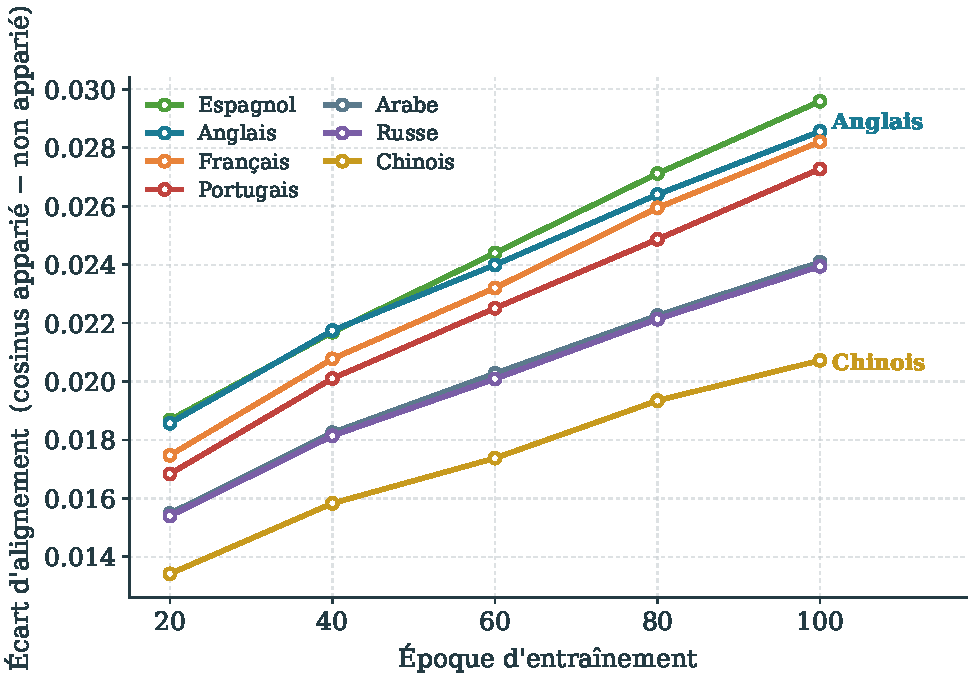
\includegraphics[width=0.74\textwidth]{figures/fig_gap_vs_epoch.pdf}
\caption{Écart d'alignement (cosinus apparié $-$ non apparié) en fonction de
l'époque, une courbe par langue, CE contrastif. L'écart croît de façon monotone
dans chaque langue, sans plateau. L'ordre
$\text{es}\approx\text{en}>\text{fr}>\text{pt}>\text{ar}\approx\text{ru}>\text{zh}$
est \emph{identique à chaque point de contrôle}~: c'est une structure, et non du
bruit. Le chinois accuse un retard de 28\,\% sur l'anglais à l'époque~100.}
\label{fig:gap}
\end{figure}

L'ordre inter-lingue se maintient à chaque point de contrôle, et l'entraînement
long (300 époques) ne montre aucun plateau. La récupération à 300 époques (lot~128)
atteint R@1 $0{,}068$, R@3 $0{,}174$, R@10 $0{,}340$, contre un hasard de
$0{,}002/0{,}006/0{,}020$. L'alignement est réel et bien au-dessus du hasard, là
où le cosinus n'en produisait aucun.

\paragraph{Interprétation.} Deux propriétés de ces courbes méritent d'être
soulignées. La \emph{monotonie}~: l'écart ne cesse de croître jusqu'à 300 époques,
ce qui indique que le budget d'entraînement, et non la capacité du modèle, limitait
encore l'alignement. La \emph{stabilité de l'ordre}~: les langues ne se croisent
jamais, ce qui exclut que les différences soient du bruit d'entraînement. Le fait que
l'espagnol rattrape, voire dépasse, l'anglais est cohérent avec la proximité des
langues romanes et la qualité de la traduction vers l'espagnol~; le retard du
chinois, de son côté, est cohérent avec la distance linguistique et la plus grande
difficulté de la traduction automatique vers cette langue.

\section{Le compromis génération--discrimination}
\label{sec:tradeoff}

L'objectif contrastif qui répare l'alignement \emph{coûte} de la qualité de
génération. Le tableau~\ref{tab:tradeoff} place les deux objectifs côte à côte.

\begin{table}[ht]
\centering
\caption{Le compromis génération--discrimination. \textbf{Évaluateur~B}. Le CE
contrastif achète l'alignement et la récupération au prix du FID.}
\label{tab:tradeoff}
\small
\begin{tabular}{@{}lrrrr@{}}
\toprule
Objectif & écart (en) & R@10 & FID$\downarrow$ & Diversité \\
\midrule
cosinus                & 0,0002 & 0,024 & \textbf{55,864} & -- \\
contrastif CE, 300 ép. & \textbf{0,0286} & \textbf{0,340} & 72,902 & 0,922 \\
mouvement réel         & -- & -- & 0,000 & 9,675 \\
\bottomrule
\end{tabular}
\end{table}

\textbf{Pourquoi ils se dissocient~:} l'InfoNCE ne contraint que le \emph{classement}
des paires appariées contre non appariées, une propriété sans échelle et purement
directionnelle. Il n'exige jamais que le latent conserve assez d'information pour
\emph{reconstruire} un mouvement distinct, seulement assez pour être
\emph{distinguable}. Une représentation peut donc être très discriminante et mal
décodable en même temps. On a par ailleurs vérifié que ce n'est pas une inadéquation
d'échelle~: renormaliser les embeddings de texte à la norme du latent ($20{,}413$
contre $9{,}232$) ne change le FID que de $2{,}1$ ($72{,}902\to70{,}786$).

\paragraph{Une image pour s'en souvenir.} On peut se représenter la différence
ainsi~: le contrastif apprend au modèle à \emph{reconnaître} un mouvement parmi
d'autres, comme on reconnaît un visage dans une foule sans pouvoir le dessiner. La
génération, elle, demande de savoir \emph{dessiner}. Les deux compétences sont
liées, mais l'une n'implique pas l'autre~: c'est exactement ce que mesure le
tableau~\ref{tab:tradeoff}.

\section{L'effondrement de l'amplitude du mouvement}
\label{sec:amplitude}

L'échec de génération le plus lourd de conséquences est l'effondrement des
mouvements vers une pose quasi statique. À l'aide du diagnostic d'amplitude, le
tableau~\ref{tab:amplitude} montre l'amplitude \emph{décroître} à mesure que les
modèles s'entraînent plus longtemps et s'améliorent sur toutes les autres
métriques.

\begin{table}[ht]
\centering
\caption{Amplitude du mouvement (différence absolue moyenne image-à-image) et
différence entre \emph{prompts} (marche contre saut). Les modèles mieux entraînés
bougent moins.}
\label{tab:amplitude}
\small
\begin{tabular}{@{}llrrr@{}}
\toprule
Modèle & époques & amplitude & marche/saut & ratio \\
\midrule
vae-en-mu-kl1e-3 (cosinus) & 20  & \textbf{0,0768} & 0,1127 & 1,5 \\
vel10-test                & 60  & 0,0145 & 0,0526 & 3,6 \\
ce150-combined            & 150 & 0,0108 & 0,0409 & 3,8 \\
ce150-all                 & 150 & 0,0063 & --    & -- \\
vae-ml-sampled-ft         & 330 & 0,0044 & 0,0204 & 4,6 \\
\bottomrule
\end{tabular}
\end{table}

Trois explications sont écartées, une à une. \textbf{(1)~Ce n'est pas un artefact
de rendu}~: le point de contrôle à 20 époques affiche des poses visiblement
différentes selon le \emph{prompt} via le même script. \textbf{(2)~Ce n'est pas
une inadéquation d'échelle des embeddings}~: la renormalisation a rendu l'amplitude
\emph{pire} ($0{,}01075\to0{,}00607$). \textbf{(3)~Ce n'est pas le poids de la
vitesse}~: à époques appariées, $\lvel=10$ donne légèrement \emph{moins} d'amplitude
que $\lvel=100$. Ce qu'il \emph{est}~: une décroissance monotone au sein d'un même
entraînement, tout le reste étant fixé (figure~\ref{fig:ampdecay}).

\begin{figure}[ht]
\centering
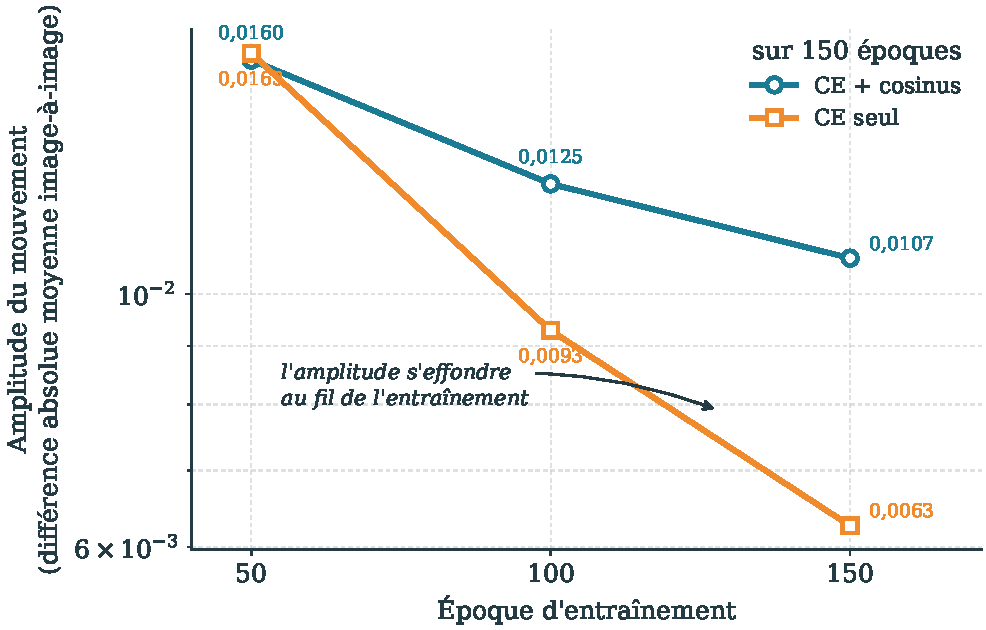
\includegraphics[width=0.64\textwidth]{figures/fig_amplitude_decay.pdf}
\caption{Amplitude du mouvement en fonction de l'époque pour deux entraînements
(axe $y$ logarithmique). L'amplitude décroît de façon monotone à mesure que
l'entraînement progresse. Le modèle « meilleur » à 20 époques du
tableau~\ref{tab:amplitude} est simplement \emph{moins convergé}~: sa forte
amplitude est de la variance sous-entraînée, non un mouvement supérieur.}
\label{fig:ampdecay}
\end{figure}

\textbf{Interprétation.} La reconstruction MSE pousse le décodeur vers des moyennes
conditionnelles~; moyennée sur un mouvement groupé, cette moyenne est une pose
debout quasi statique. Les points de contrôle précoces n'y ont pas encore convergé
et produisent donc encore de la variation. Ceci est directement visible sur les
squelettes générés (figure~\ref{fig:skeleton}), qui bougent à peine sur 60~images.
On a par ailleurs vérifié que l'\emph{encodeur} est sain~: le cosinus
mouvement--mouvement sur 200 clips couvre $0{,}31$--$0{,}98$ (moyenne $0{,}61$)~;
l'effondrement est du côté \emph{décodeur}, et uniquement sur le chemin conditionné
par le texte.

\paragraph{Pourquoi la moyenne est une pose immobile.} L'argument peut être rendu
précis. Pour une perte quadratique, la prédiction optimale d'un décodeur qui ne
dispose que d'une information partielle $c$ sur le clip est la \emph{moyenne
conditionnelle} $\E[x\mid c]$. Si $c$ ne détermine pas la phase du mouvement
(à quel instant le pied gauche se lève, par exemple), cette moyenne fait la moyenne
de mouvements \emph{déphasés}~: les oscillations s'annulent et il ne reste que la
pose centrale. Plus l'entraînement converge vers cet optimum, plus le mouvement
généré s'immobilise~; c'est exactement la décroissance monotone observée. Un modèle
génératif véritable doit au contraire \emph{échantillonner} une phase particulière,
ce que permettent la diffusion ou les tokens discrets, mais pas une régression MSE
depuis un latent unique.

\begin{figure}[ht]
\centering
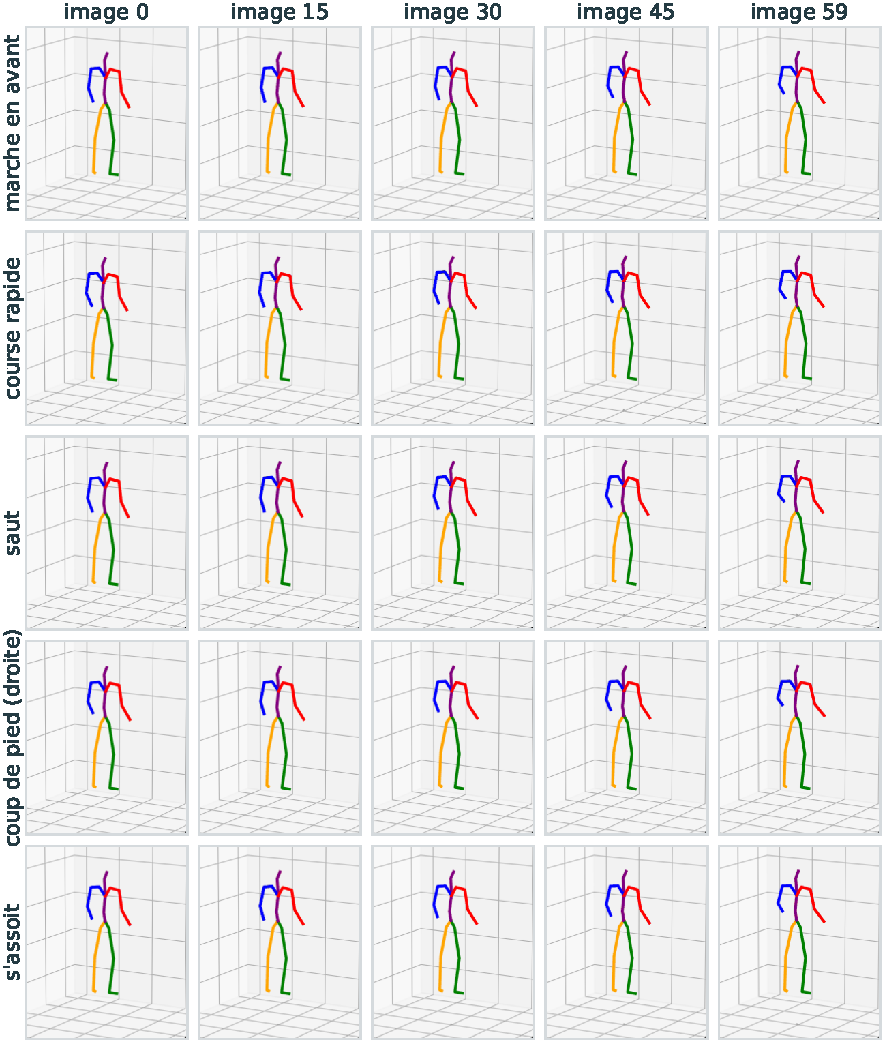
\includegraphics[width=0.78\textwidth]{figures/fig_skeleton_grid.pdf}
\caption{Squelettes générés, cinq \emph{prompts} (lignes) échantillonnés à cinq
instants (colonnes) depuis un modèle entraîné, caméra et cadrage fixes. Au sein de
chaque ligne, la pose change à peine sur les 60~images, et d'une ligne à l'autre
les poses sont quasi identiques~: l'effondrement de l'amplitude rendu visible.}
\label{fig:skeleton}
\end{figure}

\section{Reconstruction conditionnée par le texte}
\label{sec:textrc}

Le décodeur n'est entraîné que sur les latents de mouvement $\mu$, alors qu'à la
génération il reçoit un embedding de \emph{texte} $e_{\text{texte}}$
(figure~\ref{fig:arch}). Cette substitution n'est jamais optimisée. On ajoute donc
un terme qui entraîne exactement le chemin utilisé à la génération~:
\begin{equation}
\mathcal{L}_{\text{text-rc}} \;=\; \lVert D(e_{\text{texte}}) - x\rVert^2 .
\end{equation}
Le tableau~\ref{tab:textrc} rapporte des résultats à 150 époques.

\begin{table}[ht]
\centering
\caption{Reconstruction conditionnée par le texte et choix de l'encodeur,
150 époques. «~marche/saut~» est la différence entre \emph{prompts} (force du
conditionnement).}
\label{tab:textrc}
\small
\begin{tabular}{@{}llclrr@{}}
\toprule
Entraînement & text\_rc & encodeur & amplitude & marche/saut & ratio \\
\midrule
ce150-combined  & non & M-CLIP   & 0,0108 & 0,0409 & 3,8 \\
wk-rc20         & non & M-CLIP   & 0,0078 & 0,0376 & 4,8 \\
\textbf{wk-textrc}      & \textbf{oui} & M-CLIP   & 0,0042 & \textbf{0,2456} & \textbf{58} \\
\textbf{wk-textrc-rc20} & \textbf{oui} & M-CLIP   & 0,0030 & \textbf{0,2933} & \textbf{99} \\
wk-perlang      & non & par langue & \textbf{0,0174} & 0,0934 & 5,4 \\
wk-perlang-comb & non & par langue & \textbf{0,0192} & 0,0972 & 5,1 \\
\bottomrule
\end{tabular}
\end{table}

Deux constats en découlent. \textbf{Le conditionnement textuel a augmenté d'un
facteur 6--7} ($0{,}041\to0{,}293$)~: le décodeur répond désormais fortement à la
phrase qu'on lui donne. Mais l'amplitude a encore chuté, à $0{,}003$~: le terme
récompense la bonne \emph{pose} pour un clip, non la \emph{trajectoire}, puisqu'un
seul embedding de texte doit expliquer les 60~images. Le correctif naturel,
appliquer aussi le terme de vitesse à la sortie conditionnée par le texte, est
proposé mais non encore réalisé. Par ailleurs, \textbf{le banc d'encodeurs par
langue donne 2--3$\times$ plus d'amplitude} que M-CLIP à réglages appariés
($0{,}017$--$0{,}019$ contre $0{,}006$--$0{,}011$). Ceci \emph{inverse} le verdict
apparent de la section~\ref{sec:perlang-first}, obtenu sous l'objectif cosinus
défectueux et qui ne mesurait donc jamais ce qu'il semblait mesurer.

\section{Comparaison contrôlée~: EN / Latines / Éloignées / Toutes}
\label{sec:controlee}

On en vient enfin à la question du stage. Toutes les conditions sont entraînées
sur 150 époques, lot~128, CE contrastif, $\lkl=10^{-3}$, encodeur M-CLIP,
\emph{identiques en tout point sauf l'ensemble de langues}. L'alignement est mesuré
sur 500 clips à légendes parallèles~; la génération via l'évaluateur de Guo,
20 réplications.

\begin{table}[ht]
\centering
\caption{Comparaison contrôlée. Toutes les conditions identiques sauf l'ensemble
de langues. R@1 anglais, écart anglais, dispersion inter-lingue et génération.
Meilleure valeur par colonne en gras.}
\label{tab:controlee}
\small
\begin{tabular}{@{}llrrrrr@{}}
\toprule
Condition & langues & en R@1 & écart en & disp. & FID$\downarrow$ & Diversité \\
\midrule
EN              & en          & \textbf{0,610} & \textbf{0,0515} & 0,0398 & 67,660 & \textbf{1,800} \\
Latines         & en fr es pt & 0,410 & 0,0372 & 0,0253 & 95,969 & 0,668 \\
Éloignées       & en ru zh ar & 0,316 & 0,0336 & 0,0096 & \textbf{63,924} & 0,760 \\
Toutes          & 7 langues   & 0,316 & 0,0334 & 0,0071 & 74,035 & 0,831 \\
Toutes + cosinus& 7 langues   & 0,266 & 0,0289 & \textbf{0,0066} & 74,479 & 1,459 \\
mouvement réel  & --          & 0,529 & --    & --    & 0,000 & ${\sim}9,5$ \\
\bottomrule
\end{tabular}
\end{table}

\textbf{Le conditionnement multilingue dégrade l'anglais de façon monotone.} La
R@1 anglaise chute $0{,}610\to0{,}410\to0{,}316$ à mesure que l'on ajoute des
langues, et la diversité tombe de $1{,}800$ à $0{,}73$--$0{,}83$ pour chaque
condition multilingue. Ceci soutient l'hypothèse de \emph{l'espace partagé
appauvri} plutôt que celle de la supervision enrichie~: les langues ajoutées
induisent une contention de capacité plutôt qu'un apport d'information
complémentaire sur la manière, la trajectoire ou l'aspect.

\begin{encadre}
\textbf{Le facteur de confusion, rappelé.} À nombre de pas de gradient fixé, chaque
clip est vu en anglais environ $1/N$ du temps sous un régime à $N$ langues. Le
calcul est apparié~; l'\emph{exposition} par langue ne l'est pas. Toute dégradation
de l'anglais peut refléter une exposition anglaise réduite plutôt que le
multilinguisme en tant que tel.
\end{encadre}

\textbf{Mais la dégradation n'est pas générale~: la capacité est divisée, non
perdue.} Le tableau~\ref{tab:controleeperlang} montre que chaque condition est la
meilleure exactement sur les langues qu'elle a vues.

\begin{table}[ht]
\centering
\caption{R@1 par langue selon la condition d'entraînement. Chaque condition est
la meilleure sur ses propres langues~; «~Toutes~» achète la couverture la plus
uniforme au prix de la performance de pointe. Meilleure valeur par langue en gras.}
\label{tab:controleeperlang}
\small
\begin{tabular}{@{}lrrrrrrr@{}}
\toprule
condition & en & fr & es & pt & ru & zh & ar \\
\midrule
EN       & \textbf{0,610} & 0,182 & 0,188 & 0,198 & 0,118 & 0,066 & 0,084 \\
Latines  & 0,410 & \textbf{0,388} & \textbf{0,430} & \textbf{0,438} & 0,150 & 0,100 & 0,086 \\
Éloignées& 0,316 & 0,150 & 0,172 & 0,144 & \textbf{0,288} & \textbf{0,238} & \textbf{0,260} \\
Toutes   & 0,316 & 0,272 & 0,294 & 0,298 & 0,248 & 0,172 & 0,184 \\
\bottomrule
\end{tabular}
\end{table}

\begin{figure}[ht]
\centering
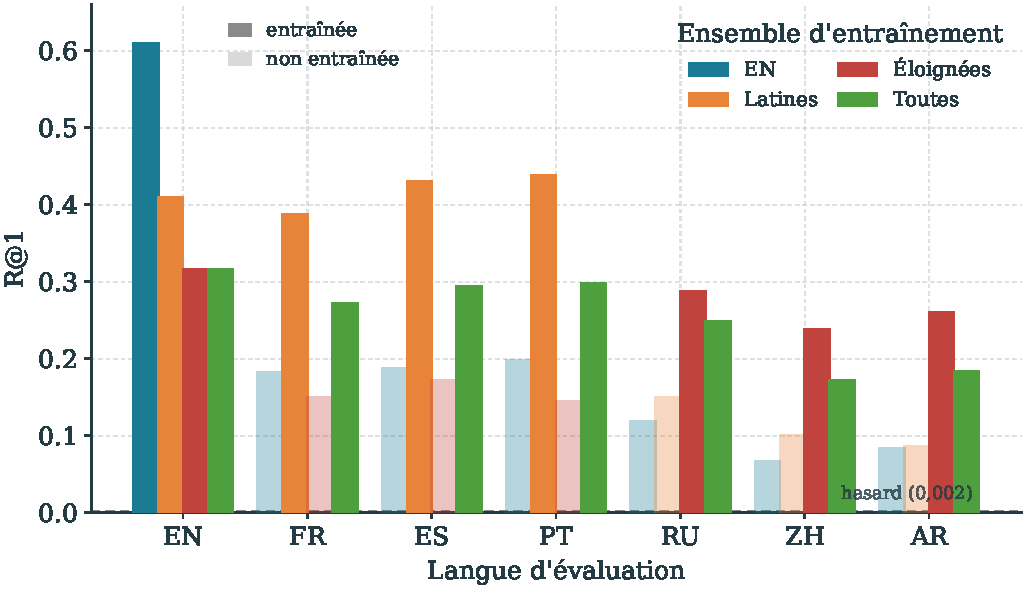
\includegraphics[width=0.74\textwidth]{figures/fig_lang_r1.pdf}
\caption{R@1 par langue selon les quatre conditions de langues. Latines rehausse
fr/es/pt~; Éloignées rehausse ru/zh/ar~; Toutes donne la couverture la plus
uniforme. Chaque groupe de barres culmine sur les langues de sa condition~: un
compromis couverture/qualité, et non une dégradation. Ligne pointillée~: hasard
($0{,}002$).}
\label{fig:langr1}
\end{figure}

Deux observations secondaires closent la comparaison. \textbf{Les langues non
entraînées restent bien au-dessus du hasard}~: le modèle Latines atteint R@1
$0{,}100$ en chinois ($50\times$ le hasard) sans avoir jamais vu une légende
chinoise, ce qui est le transfert inter-lingue pré-entraîné de M-CLIP transparaissant
à travers l'encodeur gelé. \textbf{Les Éloignées obtiennent le meilleur FID}
($63{,}924$) malgré un alignement plus faible que les Latines, ce qui est cohérent
avec la dissociation de la section~\ref{sec:tradeoff}.

\textbf{Le terme cosinus restaure la diversité.} C'est le résultat pratique le plus
net de la comparaison. Ajouter le terme cosinus à l'objectif contrastif
(\emph{Toutes + cosinus}) \emph{double} à peu près la diversité, de $0{,}73$--$0{,}83$
à $1{,}459$, à FID essentiellement inchangé ($74{,}479$ contre $74{,}035$). C'est
exactement le mécanisme de la section~\ref{sec:tradeoff}~: le CE contrastif, sans
échelle, ne contraint que le classement et ne force donc pas une sortie de pleine
amplitude~; le terme cosinus fournit la contrainte absolue manquante (élevant la
similarité moyenne de ${\sim}0{,}10$ à ${\sim}0{,}55$) tandis que le CE fournit la
séparation par échantillon que le cosinus seul ne produit jamais. \textbf{Les deux
objectifs sont complémentaires, et la perte combinée est la configuration
recommandée}~: diversité quasi optimale, couverture inter-lingue la plus uniforme
(dispersion $0{,}0066$), au prix d'un modeste recul de la récupération anglaise de
pointe.

\section{Analyse qualitative et des erreurs}
\label{sec:erreurs}

Au-delà des métriques agrégées, une inspection qualitative des mouvements générés
éclaire la \emph{nature} des défaillances et confirme les interprétations
quantitatives.

\paragraph{Ce que le modèle réussit.} Pour des \emph{prompts} simples et fréquents
dans le corpus (« une personne marche », « une personne s'assoit »), le modèle
conditionné par le texte (avec le terme \texttt{text\_rc}) produit des poses
globalement correctes et distinctes d'un prompt à l'autre, comme en témoigne la
forte différence inter-prompts (jusqu'à un ratio marche/saut de~99,
section~\ref{sec:textrc}). La sémantique de haut niveau --- la \emph{posture}
associée à une action --- est donc bien capturée.

\paragraph{Ce que le modèle échoue à produire.} La défaillance dominante est
l'absence de \emph{trajectoire}~: au sein d'un clip, le mouvement reste quasi
immobile (figure~\ref{fig:skeleton}). Le modèle génère une « photographie » de
l'action plutôt qu'une « vidéo ». Ce constat est cohérent avec l'analyse de la
section~\ref{sec:textrc}~: un unique embedding de texte doit expliquer les
60~images, et la reconstruction MSE le pousse à optimiser la pose moyenne plutôt
que la dynamique. On s'attend donc à ce que les actions intrinsèquement
dynamiques (courir, sauter, donner un coup de pied) soient les plus pénalisées, et
les actions quasi statiques (se tenir debout, s'asseoir) le moins~; la
figure~\ref{fig:skeleton} va dans ce sens (course et saut y sont méconnaissables),
mais une mesure d'amplitude \emph{par action} reste à faire pour l'établir.

\paragraph{Erreurs spécifiques au multilinguisme.} Pour les langues à écriture non
latine, et en particulier le chinois, l'alignement plus faible
(section~\ref{sec:contrastive}) se traduit par une récupération moins fiable de la
bonne légende (R@1 plus faible, tableau~\ref{tab:controleeperlang}). L'encodeur de
texte n'en est pas la cause probable, puisque M-CLIP aligne très bien les
embeddings entre langues (section~\ref{sec:cosfail})~; l'explication la plus
cohérente avec nos mesures est la capacité réduite par langue du latent de
mouvement sous entraînement multilingue. Une analyse des confusions \emph{par
action} n'a pas été menée.

\paragraph{Diagnostic global.} Les trois familles d'erreurs sont compatibles avec
une même cause structurelle~: la compression en un latent unique. L'analyse qualitative
ne contredit jamais les métriques~; elle en précise la portée et oriente vers la
solution architecturale du chapitre~\ref{ch:discussion}.

\section{Robustesse et reproductibilité}
\label{sec:robust}

Deux précautions renforcent la fiabilité des conclusions. D'une part, chaque
métrique de génération est moyennée sur \textbf{20 réplications}~: la variance
inter-réplications de l'évaluateur est de l'ordre de $0{,}002$ en diversité, bien
inférieure aux écarts discutés (par exemple le passage de $0{,}83$ à $1{,}459$ en
diversité avec le terme cosinus). D'autre part, les écarts d'alignement sont
calculés sur \textbf{500 clips} à légendes parallèles, le hasard pour R@1 étant de
$0{,}002$~; les valeurs rapportées (jusqu'à R@10 $=0{,}340$) sont donc deux ordres
de grandeur au-dessus du hasard. Enfin, l'un des enseignements méthodologiques du
stage (section~\ref{sec:bugs}) est que \emph{les pertes d'entraînement ne sont pas
des preuves}~: toutes les conclusions reposent sur des métriques d'évaluation
dédiées, et non sur l'allure des courbes de perte.

% =====================================================================
% CHAPITRE 6 : DISCUSSION
% =====================================================================
\chapter{Discussion, limites et perspectives}
\label{ch:discussion}

\section{Ce que les mesures établissent}

Quatre affirmations sont étayées par les éléments qui précèdent. \textbf{(1)} Dans
un VAE de mouvement à latent unique, c'est l'échantillonnage, et non la force du
KL, qui constitue la contrainte liante sur la reconstruction
(section~\ref{sec:kl})~; la proposition~\ref{prop:jacobien}
(section~\ref{sec:goulot}) en donne la raison. \textbf{(2)} L'objectif cosinus ne
produit aucun alignement par échantillon, quel que soit son poids, alors qu'un
objectif contrastif produit un alignement réel, monotone et structuré entre
langues (sections~\ref{sec:cosfail}--\ref{sec:contrastive}). \textbf{(3)}
L'alignement et la qualité de génération se dissocient (section~\ref{sec:tradeoff}).
\textbf{(4)} Sous reconstruction MSE, l'amplitude de génération décroît vers une
pose moyenne (section~\ref{sec:amplitude}), et le conditionnement multilingue
divise un budget représentationnel fixe plutôt que de l'enrichir
(section~\ref{sec:controlee}). La seule recommandation de conception clairement
\emph{positive} est la perte combinée CE + cosinus, qui restaure la diversité sans
coût en FID.

\section{Menaces à la validité}
\label{sec:threats}

Cette section est délibérément franche~; c'est elle qui rend le reste crédible.

\begin{itemize}[leftmargin=*]
\item \textbf{Légendes traduites par machine}~: elles mêlent les artefacts de
traduction à une véritable variation typologique. Aucune légende non anglaise
rédigée par un humain n'existe dans cette étude.
\item \textbf{L'exposition par langue n'est pas appariée}~: sous $N$ langues,
chaque clip est vu dans une langue donnée ${\sim}1/N$ du temps à nombre de pas de
gradient fixé. Le calcul est apparié~; l'exposition ne l'est pas. Toute dégradation
multilingue peut refléter une exposition anglaise réduite plutôt que le
multilinguisme (section~\ref{sec:controlee}).
\item \textbf{La R-précision est anglophone par construction}~: sa tour de texte
est un GloVe BiGRU anglais. La qualité par langue est évaluée par la FID seule.
\item \textbf{\lkl{} a été comparé à zéro, non balayé.}
\item \textbf{Les courbes d'alignement n'avaient pas convergé} au budget d'époques
utilisé (figure~\ref{fig:gap}).
\item \textbf{Les valeurs de FID sont $100\times$ au-dessus des résultats HumanML3D
publiés}~; MotionCLIP est un générateur faible et le pool de validation n'est pas
le split officiel. Toutes les comparaisons de ce rapport sont relatives, non
absolues.
\item \textbf{L'affinage du VAE a changé deux variables à la fois}
(section~\ref{sec:vaefonc})~; le contrôle déterministe seul reste à mener.
\end{itemize}

\section{Explications alternatives écartées}
\label{sec:alternatives}

Une part importante de la crédibilité d'un résultat négatif tient à la rigueur avec
laquelle les explications \emph{concurrentes} ont été éliminées. Pour les deux
constats principaux, on récapitule les alternatives considérées et la raison de leur
rejet.

\paragraph{Pour l'effondrement de l'amplitude.}
\begin{itemize}[leftmargin=*]
\item \emph{Artefact de rendu}~? Non~: le même script produit des poses visiblement
distinctes sur un modèle peu entraîné (section~\ref{sec:amplitude}).
\item \emph{Inadéquation d'échelle des embeddings}~? Non~: la renormalisation à la
norme du latent \emph{aggrave} l'amplitude.
\item \emph{Poids de vitesse trop faible}~? Non~: à époques appariées, augmenter
$\lvel$ ne rétablit pas l'amplitude.
\item \emph{Encodeur défaillant}~? Non~: le cosinus mouvement--mouvement couvre
$0{,}31$--$0{,}98$, l'encodeur produit donc des latents bien séparés~; la défaillance
est côté décodeur.
\end{itemize}
Une fois ces alternatives écartées, il ne reste que l'explication retenue~: la
régression MSE vers la moyenne conditionnelle.

\paragraph{Pour la division du budget multilingue.}
\begin{itemize}[leftmargin=*]
\item \emph{Encodeur de texte multilingue de mauvaise qualité}~? Non~: M-CLIP aligne
les embeddings textuels entre langues à plus de $0{,}97$ (section~\ref{sec:cosfail}).
\item \emph{Mauvaise mesure d'alignement}~? Précisément corrigée en remplaçant la
moyenne cosinus par l'écart (section~\ref{sec:cosfail}).
\end{itemize}
Reste un facteur de confusion non éliminé, l'exposition par langue
(section~\ref{sec:threats}), que la feuille de route propose de lever.

\section{Comparaison avec la littérature}
\label{sec:litterature}

Nos conclusions dialoguent directement avec l'hypothèse courante des travaux
multilingues (section~\ref{sub:etat-art}), selon laquelle le signal multilingue
serait, au pire, neutre pour la représentation du mouvement. Sous \emph{capacité et
calcul appariés}, nous constatons au contraire une division du budget. Ce désaccord
n'est pas nécessairement contradictoire~: les approches comme
BiHumanML3D~\cite{weng2026bihumanml3d} emploient un module d'alignement inter-lingue
dédié et une architecture plus expressive, là où nous isolons volontairement l'effet
du multilinguisme sur un modèle minimal à latent unique. Autrement dit, nos
résultats n'affirment pas que le multilinguisme nuit \emph{en général}, mais qu'il
\emph{divise un budget fixe} lorsque l'architecture ne lui en offre pas davantage.
C'est exactement pourquoi la proposition prospective (section~\ref{sec:forward})
porte sur l'\emph{architecture}~: donner au modèle la capacité séquentielle qui
pourrait transformer la division du budget en enrichissement.

\section{Vers une séquence de latents}
\label{sec:forward}

Toutes les défaillances du chapitre~\ref{ch:resultats} remontent à une cause
unique~: un latent de dimension~512 \emph{unique} est le mauvais conteneur pour une
séquence de 60~images conditionnée de façon multilingue. Le goulot ne peut
absorber le bruit d'échantillonnage (équation~\eqref{eq:expansion}), un seul
embedding de texte ne peut fournir une trajectoire sur 60~images
(section~\ref{sec:textrc}), et la MSE régresse ce vecteur unique vers une pose
moyenne (section~\ref{sec:amplitude}).

Le correctif est architectural~: une \textbf{séquence de latents}. Comme le montre
la figure~\ref{fig:bottleneck}, répartir le clip sur $K$ latents à segments
disjoints rend le terme de dégradation du bruit bloc-diagonal et permet à un
embedding de texte de conditionner des segments locaux plutôt que le clip entier.
Nous prédisons spécifiquement que \textbf{l'effondrement de l'amplitude ne devrait
pas apparaître sous des latents \emph{discrets}}, car la quantification empêche la
régression vers une moyenne conditionnelle continue~: il n'existe plus de pose
statique vers laquelle moyenner. Le test naturel est \textbf{MoMask}~\cite{guo2024momask},
dont la séquence de tokens à quantification vectorielle résiduelle réalise
exactement cette conception, conditionnée par le texte M-CLIP. C'est l'expérience
suivante la plus utile~; elle invalide tous les points de contrôle produits ici,
ce qui est la raison honnête pour laquelle elle a été laissée comme proposition
prospective plutôt que lancée.

\subsection{Feuille de route technique}

La transition vers une architecture à latents séquentiels peut se décomposer en
étapes concrètes, chacune assortie d'une prédiction vérifiable~:

\begin{enumerate}[leftmargin=*]
\item \textbf{Remplacer le latent unique par une séquence de tokens discrets}
(RVQ, à la MoMask). \emph{Prédiction}~: l'effondrement de l'amplitude
(section~\ref{sec:amplitude}) disparaît, car la quantification empêche la
régression vers une pose moyenne continue.
\item \textbf{Conditionner chaque étape de génération par M-CLIP}. \emph{Prédiction}~:
le conditionnement textuel local supprime le compromis
conditionnement/trajectoire observé en section~\ref{sec:textrc}, puisqu'un
embedding de texte n'a plus à expliquer 60~images à lui seul.
\item \textbf{Reprendre la comparaison contrôlée EN / multilingue} sur cette
nouvelle base, à capacité et calcul appariés. \emph{Prédiction}~: si la division
du budget (section~\ref{sec:controlee}) persiste malgré une architecture adéquate,
elle est intrinsèque au multilinguisme sous légendes traduites~; si elle
disparaît, elle était un artefact du goulot.
\item \textbf{Apparier l'exposition par langue} (et non seulement le calcul), pour
lever le facteur de confusion de la section~\ref{sec:threats}.
\item \textbf{Introduire des légendes non anglaises rédigées par des humains},
afin de séparer les artefacts de traduction de la véritable variation typologique
(section~\ref{sub:typologie}).
\end{enumerate}

Cette feuille de route transforme les constats \emph{négatifs} du présent rapport
en hypothèses \emph{falsifiables} pour la suite~: chaque défaillance identifiée
devient un test de l'architecture proposée.

\section{Synthèse des résultats}
\label{sec:synthese}

Le tableau~\ref{tab:synthese} récapitule les constats principaux, chacun relié à
sa cause mécanistique et à la section qui l'établit.

\begin{table}[ht]
\centering
\caption{Bilan synthétique des résultats et de leur cause mécanistique.}
\label{tab:synthese}
\small
\begin{tabular}{@{}p{4.3cm}p{6.6cm}c@{}}
\toprule
\textbf{Constat} & \textbf{Cause / mécanisme} & \textbf{Section} \\
\midrule
L'échantillonnage, non le KL, casse la reconstruction &
Un latent unique alimente les 60 images~; le terme de bruit somme sur toutes
(prop.~\ref{prop:jacobien}) & \ref{sec:kl} \\
VAE fonctionnel restauré &
Entraînement déterministe puis activation de l'échantillonnage & \ref{sec:vaefonc} \\
Le cosinus n'aligne pas &
Absence de négatifs~; optimum trivial vers la direction moyenne (prop.~\ref{prop:cosine}) & \ref{sec:cosfail} \\
Le contrastif aligne, dans 7 langues &
InfoNCE contraint le classement~; écart croissant et ordonné & \ref{sec:contrastive} \\
Alignement et génération se dissocient &
InfoNCE est sans échelle~; discriminant $\ne$ décodable & \ref{sec:tradeoff} \\
Effondrement de l'amplitude &
La MSE régresse le latent vers la pose moyenne & \ref{sec:amplitude} \\
Le multilingue divise le budget &
Capacité fixe partagée entre langues (pas de signal complémentaire) & \ref{sec:controlee} \\
\textbf{CE + cosinus restaure la diversité} &
Le cosinus fournit la contrainte absolue que le CE ne donne pas & \ref{sec:controlee} \\
\bottomrule
\end{tabular}
\end{table}

% =====================================================================
% CONCLUSION GENERALE
% =====================================================================
\chapter*{Conclusion générale et perspectives}
\addcontentsline{toc}{chapter}{Conclusion générale et perspectives}
\markboth{Conclusion générale et perspectives}{Conclusion générale et perspectives}

Ce projet de fin d'année s'était donné pour but de déterminer si le conditionnement
multilingue aide ou nuit à la génération de mouvement 3D, une fois la capacité et
le calcul appariés, et si des projections par langue entraînées indépendamment
partagent un espace commun. Sous une comparaison contrôlée, les langues ajoutées
\emph{divisent} un budget représentationnel fixe~: elles améliorent la couverture
des langues sur lesquelles elles s'entraînent tout en dégradant l'anglais de façon
monotone, et elles n'apportent pas de signal de mouvement complémentaire
(section~\ref{sec:controlee}).

Parvenir à une comparaison digne de confiance a exigé de \emph{corriger la mesure
elle-même}. La moyenne cosinus texte--mouvement, diagnostic évident, est activement
trompeuse pour cette classe de modèles~: elle peut avoisiner $1{,}0$ alors que
l'alignement par échantillon est nul (section~\ref{sec:cosfail}). En la remplaçant
par l'écart apparié--non-apparié, et l'\emph{objectif} cosinus par un objectif
contrastif, on obtient un alignement qui croît de façon monotone et avec une
structure inter-lingue stable, mais au prix de la génération, car discrimination
et décodabilité se dissocient (section~\ref{sec:tradeoff}). Chemin faisant, on a
établi que c'est l'échantillonnage, et non la force du KL, qui casse un VAE de
mouvement à latent unique (section~\ref{sec:kl}), on a restauré un modèle
variationnel fonctionnel (section~\ref{sec:vaefonc}), et on a diagnostiqué un
effondrement de l'amplitude dû à la reconstruction MSE (section~\ref{sec:amplitude}).
Le seul résultat de conception positif est la perte combinée contrastif + cosinus,
qui restaure la diversité sans coût en FID et offre la couverture inter-lingue la
plus uniforme de toutes les conditions.

Ce qui reste ouvert est architectural et précis~: passer d'un latent unique à une
séquence de latents discrets, et refaire la comparaison multilingue sur MoMask
conditionné par M-CLIP. Toutes les mesures de ce rapport pointent vers cette
expérience. Le dépôt, l'index des expériences et les notes de transmission ont été
organisés de sorte qu'elle puisse être commencée dès le premier jour.

\paragraph{Perspectives élargies.} Au-delà du cas particulier de MotionCLIP,
plusieurs enseignements de ce travail dépassent le cadre strict de la génération de
mouvement. \emph{Premièrement}, la mise en garde méthodologique sur les diagnostics
trompeurs (une moyenne cosinus proche de~$1$ masquant un alignement nul) vaut pour
tout système multimodal où l'on mesure un alignement~: il faut toujours contrôler
contre des négatifs. \emph{Deuxièmement}, la distinction entre \emph{discrimination}
et \emph{décodabilité} (section~\ref{sec:tradeoff}) concerne l'ensemble des
représentations apprises par objectif contrastif~: une représentation excellente
pour la récupération n'est pas nécessairement bonne pour la génération.
\emph{Troisièmement}, la question « le multilinguisme enrichit-il ou divise-t-il~? »
se pose, au-delà du mouvement, pour toute modalité conditionnée par du texte
multilingue (image, audio, vidéo)~; la méthodologie de comparaison contrôlée
proposée ici y est directement transposable. Enfin, sur le plan sociétal, rendre ces
systèmes véritablement multilingues reste un objectif d'inclusion important, aligné
avec la mission du centre d'accueil~: ce rapport en précise les conditions
architecturales plutôt que de le déclarer acquis.

% =====================================================================
% ANNEXES
% =====================================================================
\appendix
\renewcommand{\chaptername}{Annexe}

\chapter{Détails d'implémentation et reproduction}
\label{app:impl}

\section{Matériel et configuration}
Toutes les expériences se sont exécutées sur un unique GPU NVIDIA RTX~5090
(32~Go), partagé. L'entraînement à un lot de~128 prend environ 32~s par époque.
Configuration par défaut~: lot~128, taux d'apprentissage $10^{-4}$, 60~images,
latent~512, 8~couches, GELU, $\lrc=100$, $\lvel=100$, $\lkl=10^{-3}$. Les
entraînements longs ont été détachés avec \texttt{setsid}.

\section{Commandes de reproduction}
Chaque commande reproduit le bloc de résultats correspondant~; \texttt{<run>} et
l'époque du point de contrôle se lisent dans l'annexe~\ref{app:index}.

\begingroup
\small\ttfamily\setlength{\parindent}{0pt}
\begin{quote}
\# écart d'alignement + récupération, par langue\\
python eval\_latent\_alignment.py \textbackslash\\
\hspace*{2em}-{}-ckpt exps/<run>/checkpoint\_XXXX.pth.tar \textbackslash\\
\hspace*{2em}-{}-tag <nom> -{}-n 500 -{}-text\_encoder mclip\\[6pt]
\# qualité de génération (évaluateur B)\\
python eval\_guo\_vae\_compare\_beta05.py \textbackslash\\
\hspace*{2em}-{}-model original -{}-replications 20 \textbackslash\\
\hspace*{2em}-{}-device 0 -{}-ckpt exps/<run>/checkpoint\_XXXX.pth.tar\\[6pt]
\# la comparaison contrôlée des langues (section~\ref{sec:controlee})\\
bash eval\_all.sh 2>\&1 | tee results\_all.log
\end{quote}
\endgroup

\section{Fils ouverts}
(1)~Ajouter la supervision de vitesse au chemin conditionné par le texte
(section~\ref{sec:textrc}). (2)~Mener 10 époques \emph{déterministes}
supplémentaires depuis \texttt{vae-ml-ce-s100-e300} pour contrôler l'affinage du
VAE (section~\ref{sec:vaefonc}). (3)~Balayer \lkl{}. (4)~Obtenir des légendes non
anglaises rédigées par des humains. (5)~L'architecture en séquence de latents
(section~\ref{sec:forward}).

\chapter{Index des expériences}
\label{app:index}

Chaque entraînement ayant produit un point de contrôle, avec sa configuration
clé, ce qu'il teste et son résultat principal. Les numéros de section renvoient au
chapitre~\ref{ch:resultats}.

\begingroup
\scriptsize
\setlength{\tabcolsep}{4pt}
\renewcommand{\arraystretch}{1.2}
\begin{longtable}{@{}>{\raggedright\arraybackslash}p{3.0cm}%
 >{\raggedright\arraybackslash}p{3.1cm}%
 >{\raggedright\arraybackslash}p{2.6cm}%
 >{\raggedright\arraybackslash}p{4.1cm}@{}}
\toprule
\textbf{Run} & \textbf{Config. clé} & \textbf{Teste} & \textbf{Résultat / \S} \\
\midrule
\endfirsthead
\toprule
\textbf{Run} & \textbf{Config. clé} & \textbf{Teste} & \textbf{Résultat / \S} \\
\midrule
\endhead
\bottomrule
\endfoot
\texttt{ml-en} & M-CLIP, en & baseline & FID 18,013 · \S\ref{sec:baseline} \\
\texttt{ml-latin} & M-CLIP, en/fr/es/pt & baseline multi. & FID \textbf{16,140}, meilleur · \S\ref{sec:baseline} \\
\texttt{ml-far} & M-CLIP, en/ru/zh/ar & baseline multi. & FID 18,046 · \S\ref{sec:baseline} \\
\texttt{ml-all} & M-CLIP, 7 langues & baseline multi. & FID 17,829 · \S\ref{sec:baseline} \\
\texttt{perlang-latin} & 4 BERT gelés, cosinus & encodeurs/langue & FID 24,55, R@1 0,079 · \S\ref{sec:perlang-first} (non informatif) \\
\texttt{vae-en-kl1e-5} & $\lkl{=}10^{-5}$, éch. & force KL & rc 0,524 · \S\ref{sec:kl} \\
\texttt{vae-en-kl1e-3} & $\lkl{=}10^{-3}$, éch. & force KL & rc 0,526 · \S\ref{sec:kl} \\
\texttt{vae-en-actor} & cosinus retiré & façon ACTOR & rc 0,524 · \S\ref{sec:kl} \\
\texttt{vae-en-anneal} & recuit 30 ép. & calendrier KL & rc 0,525 · \S\ref{sec:kl} \\
\texttt{vae-en-mu-kl0} & recon. depuis $\mu$, $\lkl{=}0$ & recon. dét. & FID 97,633 · \S\ref{sec:vaefonc} \\
\texttt{vae-en-mu-kl1e-3} & recon. depuis $\mu$ & recon. dét. + KL & FID \textbf{55,864} · \S\ref{sec:vaefonc} \\
\texttt{*-beta*-ft} & affinages $\beta$ & robustesse bruit & +25,5\,\% rc, FID 57,3$\to$86,8 · \S\ref{sec:noise} (fermée) \\
\texttt{vae-multilingual-mclip} & 7 langues, cosinus & alignement & écart 0,0002 · \S\ref{sec:cosfail} \\
\texttt{vae-ml-cos100} & cosinus $\times100$ & alignement & écart 0,0007 (pire) · \S\ref{sec:cosfail} \\
\texttt{vae-ml-ce} & CE, lot 64 & alignement & écart 0,0206 · \S\ref{sec:cosfail} \\
\texttt{vae-ml-ce-s100-e100} & CE, 5 points de ctrl. & écart/époque & monotone, Fig.~\ref{fig:gap} · \S\ref{sec:contrastive} \\
\texttt{vae-ml-ce-s100-e300} & CE, 6 points de ctrl. & écart, génération & FID 72,902, R@10 0,340 · \S\ref{sec:contrastive},\ref{sec:tradeoff} \\
\texttt{vae-ml-sampled-ft} & dét.-puis-éch., 330 ép. & VAE fonctionnel & rc \textbf{0,086}, amp 0,0044 · \S\ref{sec:vaefonc},\ref{sec:amplitude} \\
\texttt{vel10-test} & $\lvel{=}10$ & poids vitesse & amp 0,0145 · \S\ref{sec:amplitude} \\
\texttt{ce150-combined} & CE+cosinus, 3 pts & décroiss. amplitude & amp 0,0108 · \S\ref{sec:amplitude},\ref{sec:controlee} \\
\texttt{ce150-all} & CE, 7 langues, 3 pts & décroiss. amplitude & amp 0,0063 · \S\ref{sec:amplitude} \\
\texttt{wk-textrc} & text\_rc actif & recon. cond. texte & cond. $\times$6, amp 0,0042 · \S\ref{sec:textrc} \\
\texttt{wk-perlang(-comb)} & banc par langue, CE & choix encodeur & amp 0,017--0,019, inverse \S\ref{sec:perlang-first} · \S\ref{sec:textrc} \\
\texttt{ce150-en/latin/far/all} & CE, 150 ép., ens. langues & comparaison contrôlée & Tab.~\ref{tab:controlee} · \S\ref{sec:controlee} \\
\end{longtable}
\endgroup

\chapter{Tableaux et figures supplémentaires}
\label{app:extra}

\begin{figure}[ht]
\centering
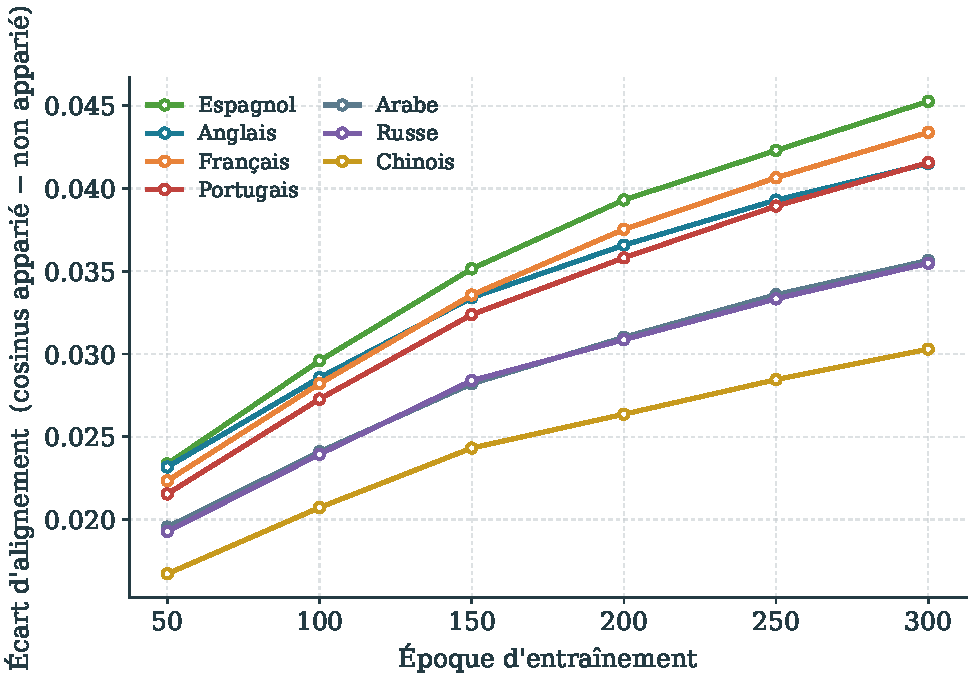
\includegraphics[width=0.74\textwidth]{figures/fig_gap_vs_epoch_300.pdf}
\caption{Écart d'alignement en fonction de l'époque sur l'entraînement long de
300 époques, une courbe par langue. Aucun plateau à 300 époques~; l'ordre
inter-lingue est le même qu'en figure~\ref{fig:gap}. C'est la preuve de la limite
«~courbes non convergées~» de la section~\ref{sec:threats}.}
\label{fig:gap300}
\end{figure}

\begin{table}[ht]
\centering
\caption{Écart d'alignement par langue selon la condition d'entraînement
(500 clips, légendes parallèles), complément du tableau~\ref{tab:controleeperlang}.}
\label{tab:controleegap}
\small
\begin{tabular}{@{}lrrrrrrr@{}}
\toprule
condition & en & fr & es & pt & ru & zh & ar \\
\midrule
EN       & 0,0515 & 0,0265 & 0,0276 & 0,0249 & 0,0215 & 0,0167 & 0,0182 \\
Latines  & 0,0372 & 0,0403 & 0,0420 & 0,0388 & 0,0232 & 0,0178 & 0,0206 \\
Éloignées& 0,0336 & 0,0248 & 0,0262 & 0,0232 & 0,0302 & 0,0268 & 0,0316 \\
Toutes   & 0,0334 & 0,0336 & 0,0351 & 0,0324 & 0,0284 & 0,0243 & 0,0282 \\
\bottomrule
\end{tabular}
\end{table}

\begin{table}[ht]
\centering
\caption{Perte combinée (CE + cosinus), cosinus apparié/non apparié et écart par
langue. Le terme cosinus élève la similarité absolue à ${\sim}0{,}55$ tout en
préservant un écart réel.}
\label{tab:combined}
\small
\begin{tabular}{@{}lrrrrrrr@{}}
\toprule
 & en & fr & es & pt & ru & zh & ar \\
\midrule
apparié    & 0,5460 & 0,5450 & 0,5460 & 0,5461 & 0,5426 & 0,5395 & 0,5430 \\
non apparié& 0,5171 & 0,5157 & 0,5153 & 0,5178 & 0,5181 & 0,5185 & 0,5187 \\
\textbf{écart} & 0,0289 & 0,0293 & 0,0307 & 0,0282 & 0,0245 & 0,0209 & 0,0243 \\
\bottomrule
\end{tabular}
\end{table}

\begin{figure}[ht]
\centering
\begin{subfigure}{0.49\textwidth}
 \centering
 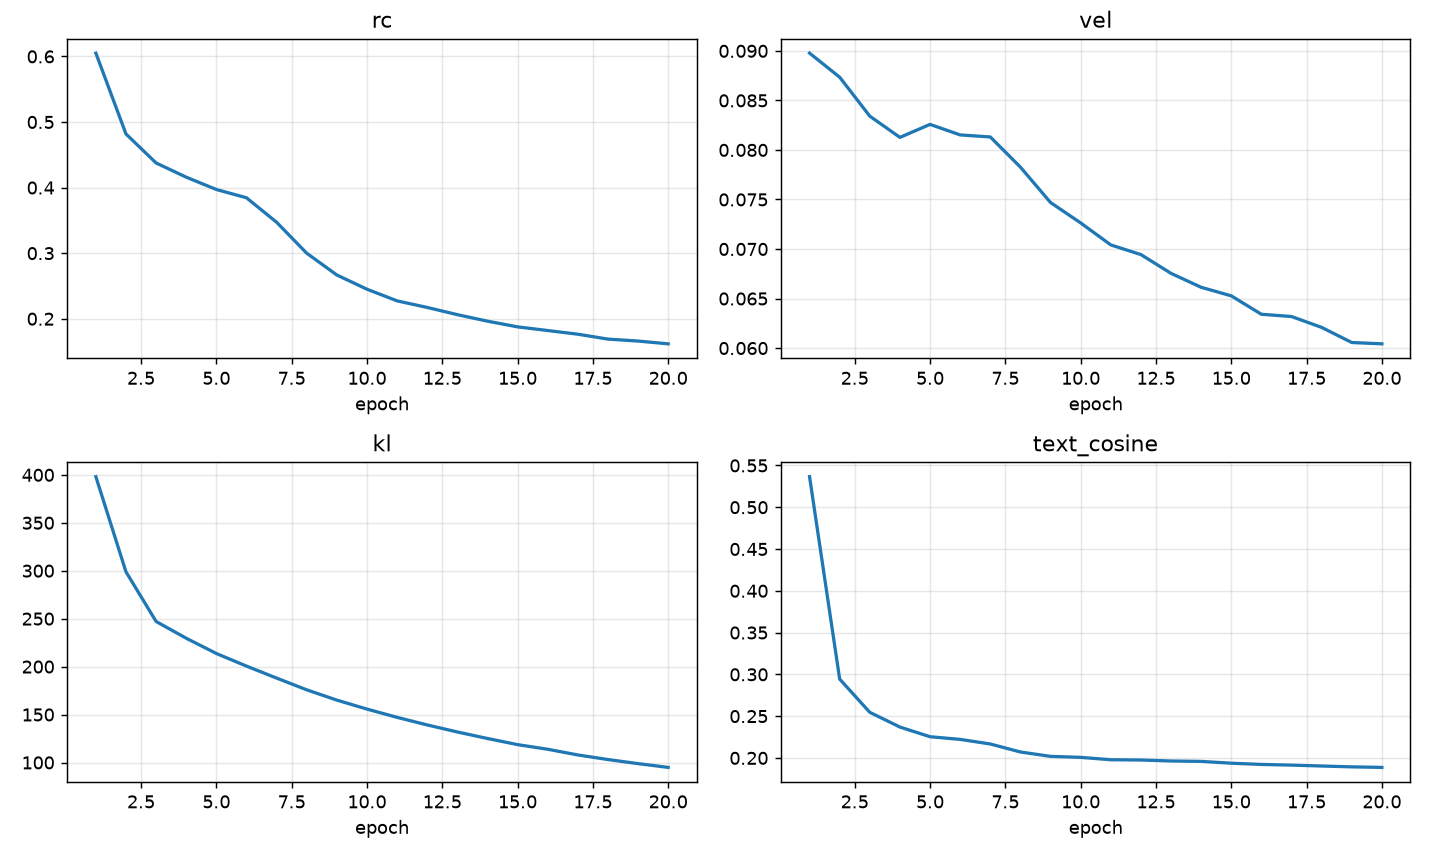
\includegraphics[width=\linewidth]{figures/curves_vae-en-mu-kl1e-3.png}
 \caption{\texttt{vae-en-mu-kl1e-3} (anglais).}
\end{subfigure}\hfill
\begin{subfigure}{0.49\textwidth}
 \centering
 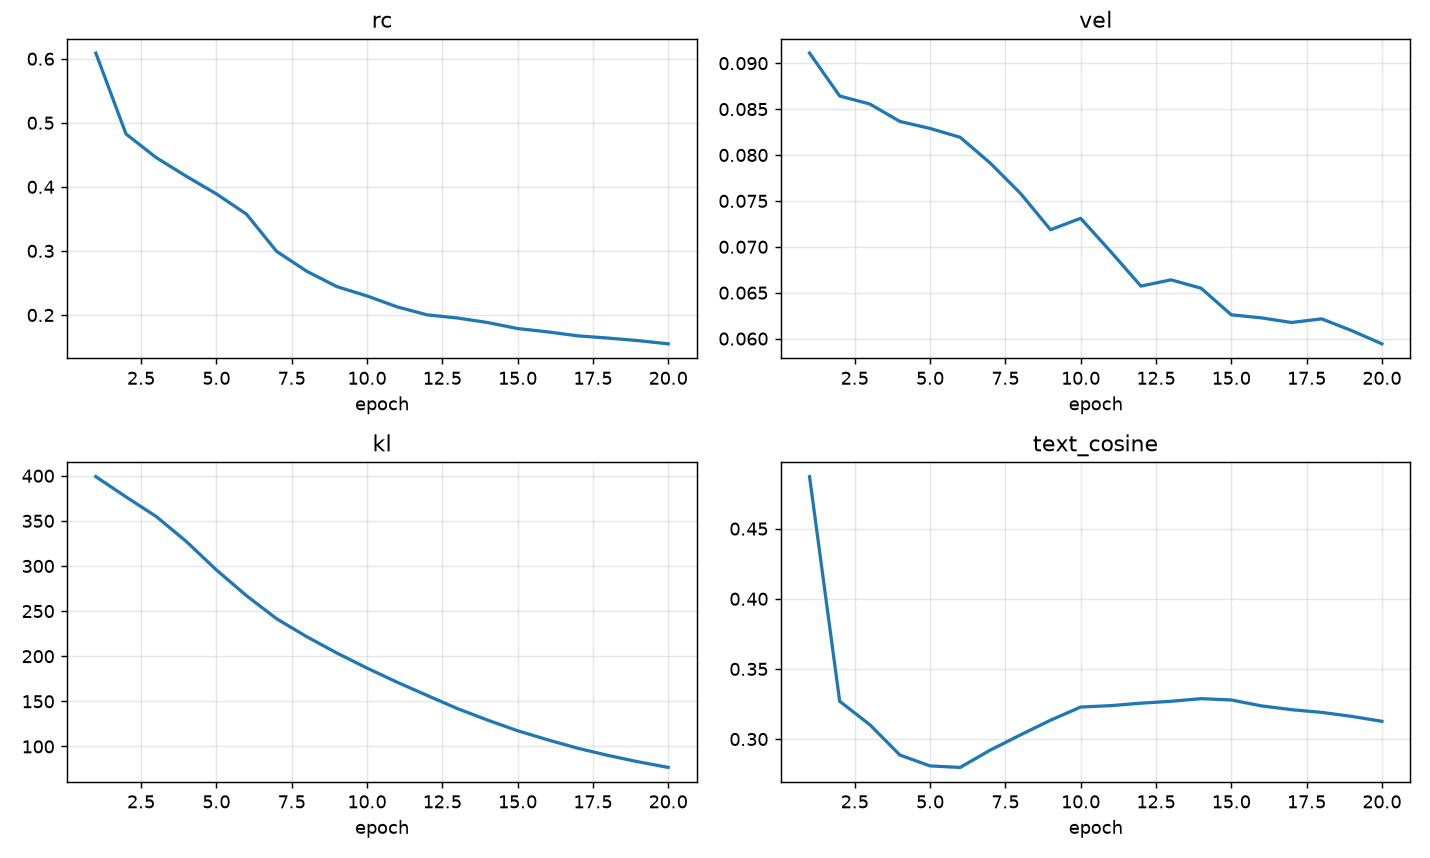
\includegraphics[width=\linewidth]{figures/curves_vae-multilingual-mclip.png}
 \caption{\texttt{vae-multilingual-mclip} (7 langues).}
\end{subfigure}
\caption{Courbes d'entraînement (rc, vel, KL, cosinus-texte) pour les VAE anglais
et multilingue. La reconstruction, la vitesse et le KL suivent des trajectoires
proches~; les deux ne divergent que sur le cosinus-texte, une différence que la
section~\ref{sec:cosfail} montre non informative sur l'alignement par échantillon.}
\label{fig:curves}
\end{figure}

\begin{figure}[ht]
\centering
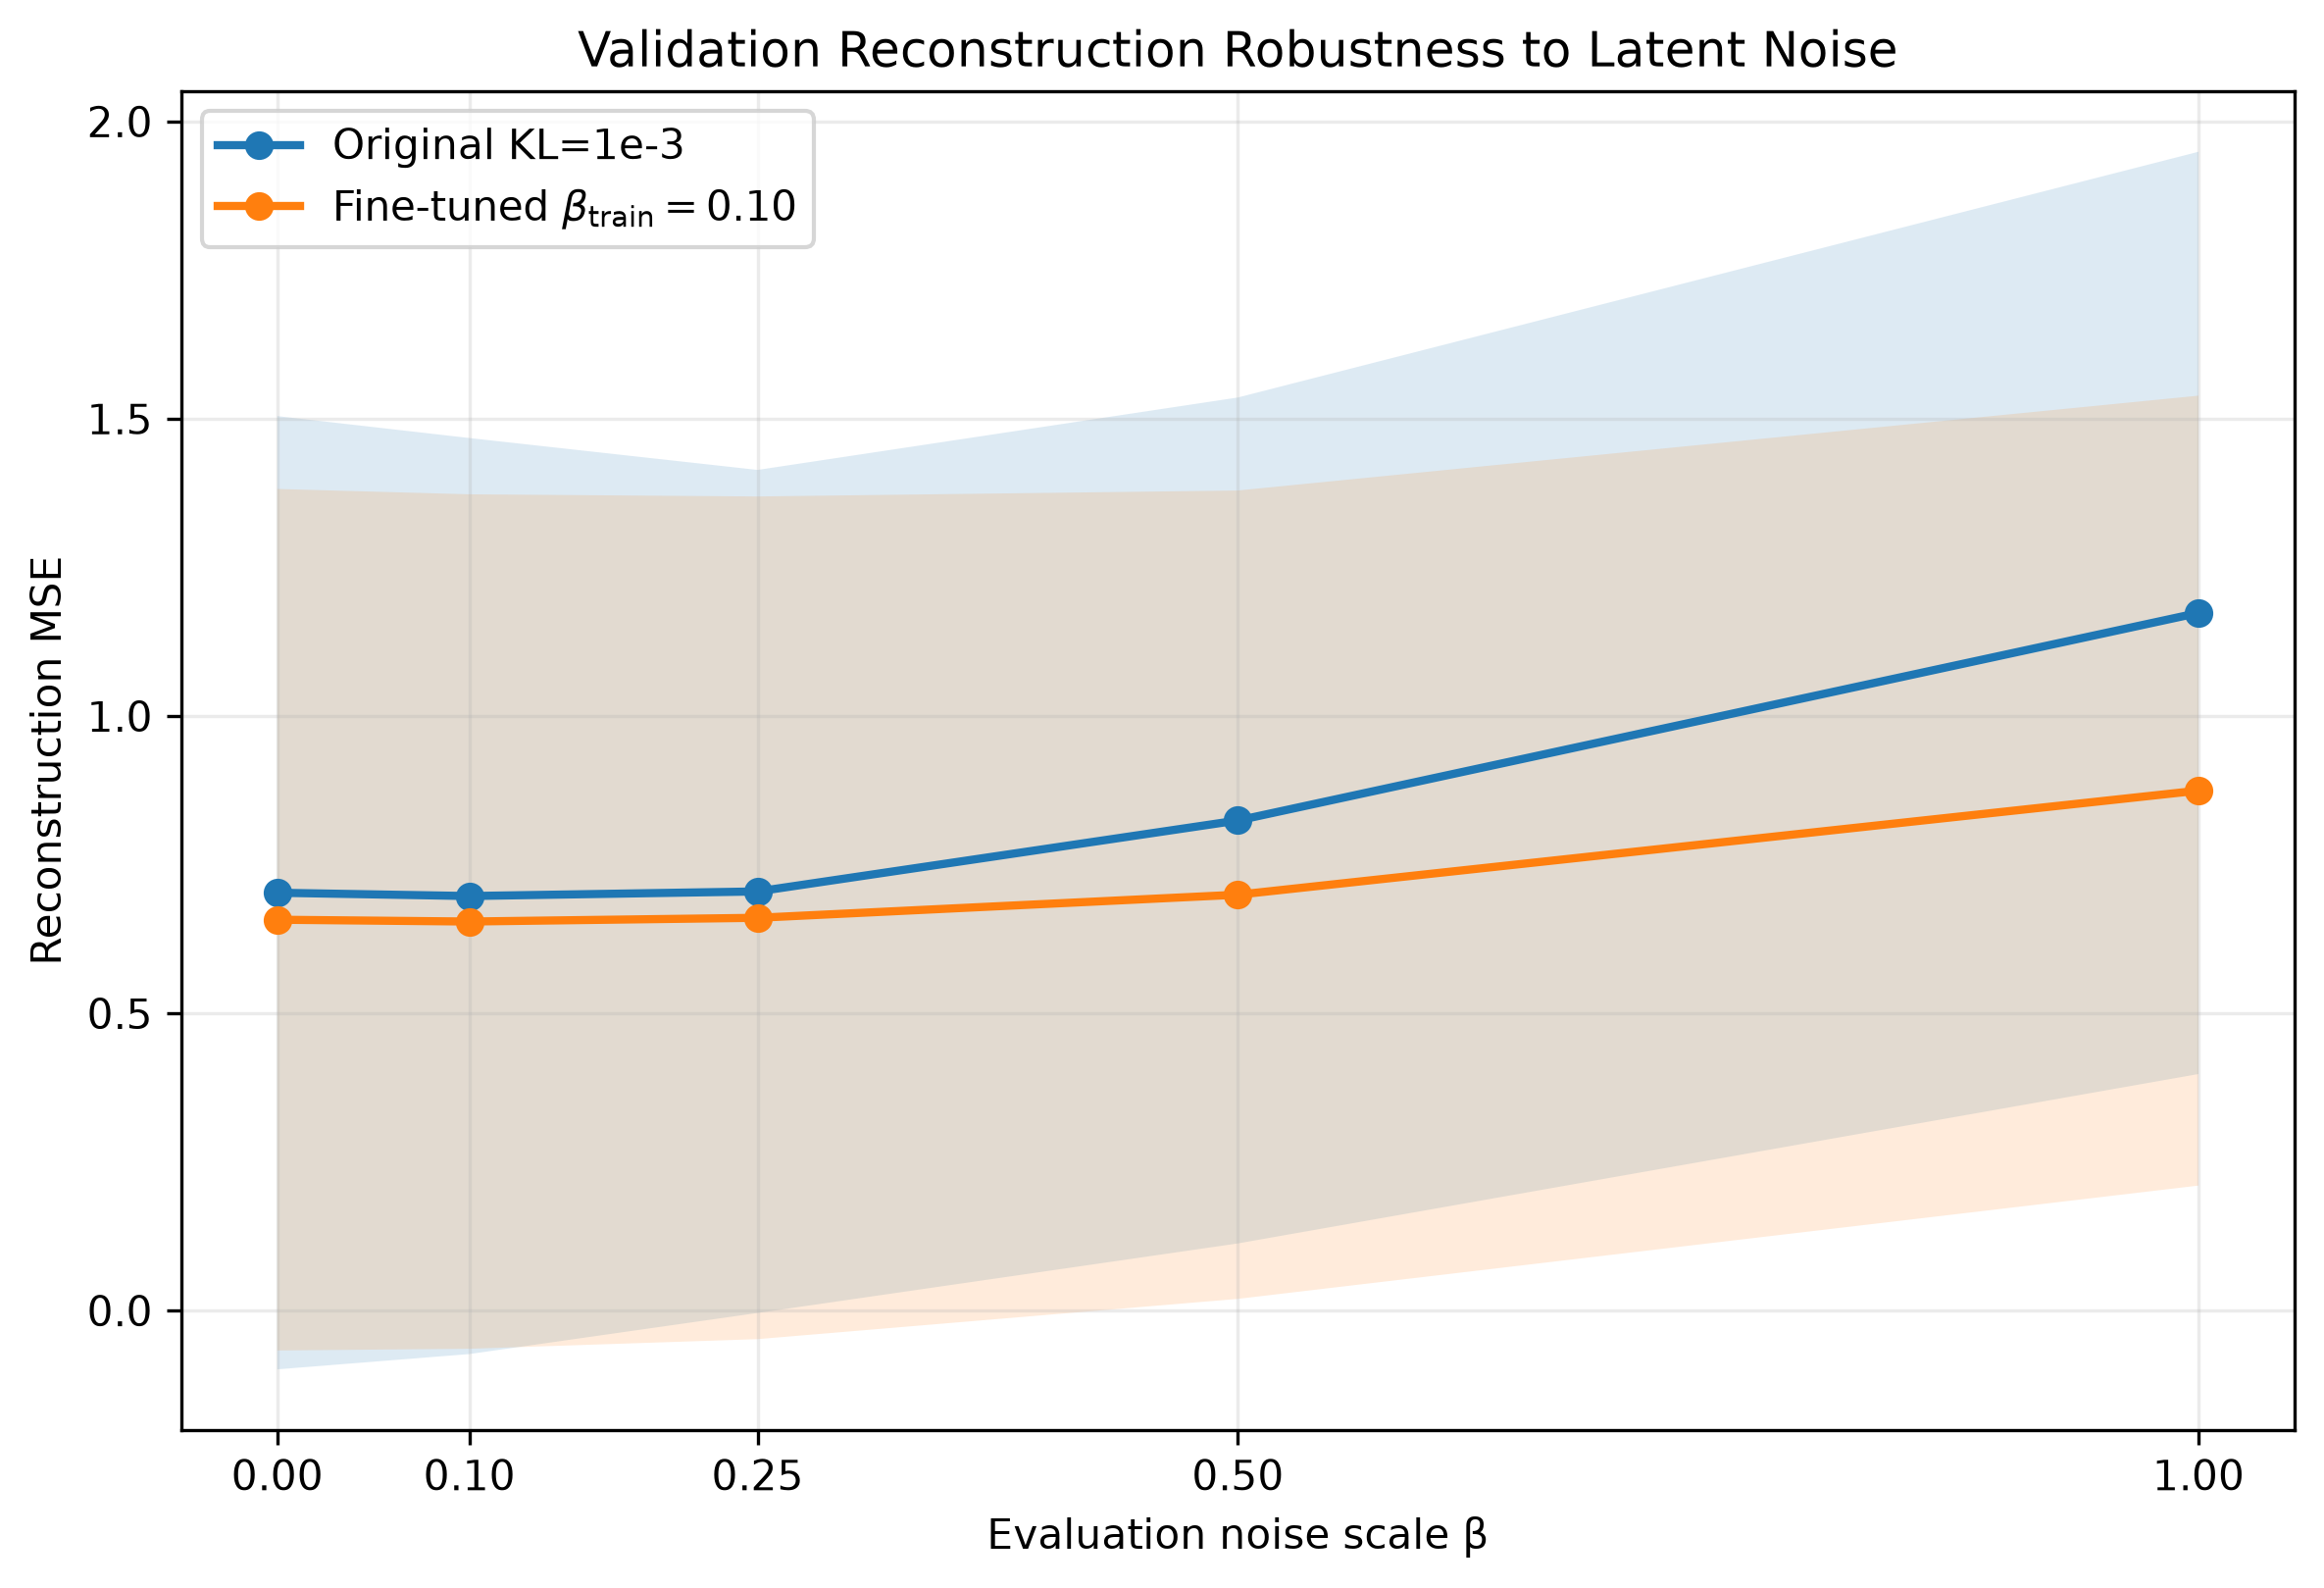
\includegraphics[width=0.72\textwidth]{figures/validation_noise_robustness.png}
\caption{Reconstruction de validation sous bruit injecté
$z=\mu+\beta\varepsilon$ pour la branche de robustesse au bruit de la
section~\ref{sec:noise}. L'affinage à $\beta=0{,}10$ améliore la reconstruction
sous bruit (les $+25{,}5\,\%$ rapportés) mais dégrade la génération
(tableau~\ref{tab:noisedown}).}
\label{fig:noise}
\end{figure}

% =====================================================================
% ANNEXE D : COMPLEMENTS MATHEMATIQUES
% =====================================================================
\chapter{Compléments mathématiques}
\label{app:math}

Cette annexe rassemble les dérivations détaillées des résultats utilisés dans le
corps du rapport.

\section{Forme close de la divergence KL gaussienne}
\label{app:kl}

On établit l'équation~\eqref{eq:kl}. La divergence de Kullback--Leibler entre deux
lois gaussiennes diagonales $q=\Ncal(\mu,\sigma^2 I)$ et $p=\Ncal(0,I)$ en dimension
$d$ s'écrit, par définition,
\begin{equation}
\KL(q\,\|\,p) = \int q(z)\log\frac{q(z)}{p(z)}\,\mathrm{d}z
= \E_{q}\big[\log q(z) - \log p(z)\big].
\end{equation}
Pour une gaussienne, $\log q(z) = -\tfrac{d}{2}\log(2\pi) - \tfrac12\sum_i\log\sigma_i^2
- \tfrac12\sum_i\frac{(z_i-\mu_i)^2}{\sigma_i^2}$ et
$\log p(z) = -\tfrac{d}{2}\log(2\pi) - \tfrac12\sum_i z_i^2$. En prenant
l'espérance sous $q$, on utilise $\E_q[(z_i-\mu_i)^2] = \sigma_i^2$ et
$\E_q[z_i^2] = \mu_i^2 + \sigma_i^2$~:
\begin{align}
\KL(q\,\|\,p)
&= \E_q\Big[-\tfrac12\textstyle\sum_i\log\sigma_i^2 - \tfrac12\sum_i\tfrac{(z_i-\mu_i)^2}{\sigma_i^2} + \tfrac12\sum_i z_i^2\Big]\\
&= -\tfrac12\textstyle\sum_i\log\sigma_i^2 - \tfrac{d}{2} + \tfrac12\sum_i(\mu_i^2+\sigma_i^2)
= -\tfrac12\sum_i\big(1 + \log\sigma_i^2 - \mu_i^2 - \sigma_i^2\big),
\end{align}
ce qui est exactement l'équation~\eqref{eq:kl}. Cette forme close évite toute
estimation de Monte-Carlo du terme de régularisation.

\section{Distance de Fréchet entre deux gaussiennes}
\label{app:fid}

La FID (équation~\eqref{eq:fid}) est la distance de Wasserstein-2 au carré entre
$\Ncal(\mu_r,\Sigma_r)$ et $\Ncal(\mu_g,\Sigma_g)$. Pour deux gaussiennes, cette
distance admet la forme close
\begin{equation}
W_2^2 = \lVert\mu_r-\mu_g\rVert^2 + \mathrm{Tr}\!\Big(\Sigma_r+\Sigma_g-2\big(\Sigma_r^{1/2}\Sigma_g\Sigma_r^{1/2}\big)^{1/2}\Big).
\end{equation}
Les matrices $\Sigma_r\Sigma_g$ et $\Sigma_r^{1/2}\Sigma_g\Sigma_r^{1/2}$ sont
semblables (la seconde s'obtient de la première par conjugaison par
$\Sigma_r^{1/2}$)~: elles ont les mêmes valeurs propres, toutes positives ou
nulles. Les traces de leurs racines carrées sont donc égales,
$\mathrm{Tr}\big(\Sigma_r^{1/2}\Sigma_g\Sigma_r^{1/2}\big)^{1/2}
= \mathrm{Tr}\,(\Sigma_r\Sigma_g)^{1/2}$, \emph{sans hypothèse de commutation},
ce qui justifie l'écriture usuelle de l'équation~\eqref{eq:fid}.
On vérifie que $W_2^2\ge0$, avec égalité si et seulement si les deux gaussiennes
coïncident~: une FID nulle correspond donc à des distributions de caractéristiques
identiques.

\section{InfoNCE comme borne de l'information mutuelle}
\label{app:infonce}

On esquisse pourquoi minimiser l'InfoNCE (équation~\eqref{eq:infonce}) maximise une
borne inférieure de l'information mutuelle $I(X;Y)$ entre les deux modalités. En
notant $f(x,y)=\exp(S_{xy}/\tau)$ le score non normalisé d'une paire, l'espérance
de la perte InfoNCE sur un lot de $B$ paires vérifie
\begin{equation}
\mathcal{L}_{\text{CE}} \;\ge\; \log B - I(X;Y),
\end{equation}
de sorte que $I(X;Y) \ge \log B - \mathcal{L}_{\text{CE}}$. Minimiser la perte relève
donc la borne sur l'information mutuelle, et la borne se resserre à mesure que la
taille de lot $B$ (donc le nombre de négatifs) augmente. Ceci éclaire un fait
observé en pratique~: la perte contrastive reste proche de $\ln B$ même lorsque
l'alignement s'améliore nettement (section~\ref{sec:bugs}), car la borne est lâche~;
seule une métrique d'évaluation dédiée révèle le progrès réel.

\section{Variance du gradient reparamétré}
\label{app:reparam}

L'intérêt de la reparamétrisation (équation~\eqref{eq:reparam}) tient aussi à la
\emph{variance} de l'estimateur du gradient. L'estimateur naïf par score
(\emph{REINFORCE}) de $\nabla_\phi\,\E_{q_\phi}[g(z)]$ a une variance qui croît avec
la dimension et rend l'apprentissage instable. L'estimateur reparamétré, en
exprimant $z=\mu+\sigma\odot\varepsilon$ avec $\varepsilon$ indépendant de $\phi$,
déplace la source d'aléa hors des paramètres et permet d'écrire
$\nabla_\phi\,\E_\varepsilon[g(\mu+\sigma\odot\varepsilon)] =
\E_\varepsilon[\nabla_\phi\,g(\mu+\sigma\odot\varepsilon)]$. Cet estimateur présente
une variance bien plus faible, ce qui explique sa supériorité empirique pour
l'entraînement des VAE.

% =====================================================================
% ANNEXE E : CONFIGURATION EXPERIMENTALE COMPLETE
% =====================================================================
\chapter{Configuration expérimentale complète}
\label{app:config}

\section{Hyperparamètres}
Le tableau~\ref{tab:hyper} liste l'ensemble des hyperparamètres par défaut. Sauf
mention contraire, toutes les expériences les reprennent, seuls variant l'ensemble
de langues, l'objectif d'alignement et l'activation de l'échantillonnage.

\begin{table}[ht]
\centering
\caption{Hyperparamètres par défaut.}
\label{tab:hyper}
\small
\begin{tabular}{@{}lll@{}}
\toprule
Catégorie & Hyperparamètre & Valeur \\
\midrule
\multirow{4}{*}{Architecture}
 & couches Transformer & 8 \\
 & dimension latente & 512 \\
 & dimension M-CLIP & 768 \\
 & activation & GELU \\
\midrule
\multirow{4}{*}{Données}
 & longueur de clip & 60 images \\
 & dimension de pose & 263 \\
 & clips d'entraînement & 22\,326 \\
 & clips de validation & 1\,400 \\
\midrule
\multirow{4}{*}{Optimisation}
 & taille de lot & 128 \\
 & taux d'apprentissage & $10^{-4}$ \\
 & $\lrc$, $\lvel$ & 100, 100 \\
 & $\lkl$ & $10^{-3}$ \\
\midrule
\multirow{3}{*}{Évaluation}
 & réplications & 20 \\
 & clips d'alignement & 500 (légendes parallèles) \\
 & langues & en, fr, es, pt, ru, zh, ar \\
\bottomrule
\end{tabular}
\end{table}

\section{Environnement logiciel et matériel}
Les expériences ont été menées avec PyTorch sur un GPU NVIDIA RTX~5090 (32~Go). Les
modèles de texte proviennent des bibliothèques \texttt{transformers} (encodeurs
monolingues) et \texttt{multilingual-clip} (M-CLIP). La traduction a été réalisée
avec NLLB. Les entraînements longs étaient détachés avec \texttt{setsid}. Chaque
résultat est accompagné, dans le dépôt, du point de contrôle et de la commande
exacte qui l'a produit (annexe~\ref{app:impl}).

\section{Détails du jeu de données}
Les clips sont extraits de HumanML3D et ramenés à une longueur fixe de 60~images
(troncature ou rejet des clips trop courts/trop longs). Chaque composante du
vecteur de 263 dimensions est standardisée à partir des statistiques du corpus
d'entraînement. Pour l'alignement inter-lingue, 500 clips disposent de légendes
\emph{parallèles} dans les sept langues, obtenues en traduisant une même légende
anglaise~; cela garantit que la seule variable entre langues est le texte, le
mouvement sous-jacent restant identique.

% =====================================================================
% ANNEXE : RESULTATS DETAILLES PAR LANGUE
% =====================================================================
\chapter{Résultats détaillés par langue}
\label{app:perlangue}

Cette annexe rassemble des tableaux complémentaires offrant une vue fine, langue par
langue, des résultats agrégés du chapitre~\ref{ch:resultats}.

\section{Écart d'alignement par langue et par époque}

Le tableau~\ref{tab:gap-detail} reprend l'évolution de l'écart d'alignement sous CE
contrastif, complétant la figure~\ref{fig:gap}. L'ordre inter-lingue
($\text{es}\approx\text{en}>\text{fr}>\text{pt}>\text{ar}\approx\text{ru}>\text{zh}$)
est strictement conservé à chaque point de contrôle.

\begin{table}[ht]
\centering
\caption{Écart d'alignement par langue et par époque (CE contrastif), valeurs
détaillées.}
\label{tab:gap-detail}
\small
\begin{tabular}{@{}rrrrrrrr@{}}
\toprule
époque & en & fr & es & pt & ru & zh & ar \\
\midrule
20  & 0,0186 & 0,0175 & 0,0187 & 0,0168 & 0,0154 & 0,0134 & 0,0155 \\
40  & 0,0217 & 0,0208 & 0,0217 & 0,0201 & 0,0181 & 0,0158 & 0,0182 \\
60  & 0,0240 & 0,0232 & 0,0244 & 0,0225 & 0,0201 & 0,0174 & 0,0203 \\
80  & 0,0264 & 0,0259 & 0,0271 & 0,0249 & 0,0221 & 0,0193 & 0,0223 \\
100 & 0,0286 & 0,0282 & 0,0296 & 0,0273 & 0,0239 & 0,0207 & 0,0241 \\
\bottomrule
\end{tabular}
\end{table}

\section{Lecture croisée R@1 et écart d'alignement}

Le tableau~\ref{tab:cross} met en regard, pour chaque condition d'entraînement, la
récupération R@1 et l'écart d'alignement en anglais. On observe que R@1 et écart
varient dans le même sens entre conditions (plus d'alignement $\Rightarrow$ plus de
récupération), ce qui confirme que l'écart apparié--non-apparié est un bon
prédicteur de la récupération, là où la moyenne cosinus ne l'était pas
(section~\ref{sec:cosfail}).

\begin{table}[ht]
\centering
\caption{Lecture croisée en anglais~: R@1 et écart d'alignement par condition.}
\label{tab:cross}
\small
\begin{tabular}{@{}lrr@{}}
\toprule
Condition & en R@1 & en écart \\
\midrule
EN        & 0,610 & 0,0515 \\
Latines   & 0,410 & 0,0372 \\
Éloignées & 0,316 & 0,0336 \\
Toutes    & 0,316 & 0,0334 \\
Toutes + cosinus & 0,266 & 0,0289 \\
\bottomrule
\end{tabular}
\end{table}

\section{Couverture par famille de langues}

Le tableau~\ref{tab:couverture} agrège la R@1 par \emph{famille}~: langues latines
(fr, es, pt) et langues éloignées (ru, zh, ar), pour chaque condition. Il rend
visible le phénomène de division du budget~: chaque condition excelle sur sa propre
famille, et « Toutes » réalise le meilleur compromis moyen.

\begin{table}[ht]
\centering
\caption{R@1 moyenne par famille de langues (hors anglais), selon la condition.}
\label{tab:couverture}
\small
\begin{tabular}{@{}lrr@{}}
\toprule
Condition & Latines (fr/es/pt) & Éloignées (ru/zh/ar) \\
\midrule
EN        & 0,189 & 0,089 \\
Latines   & \textbf{0,419} & 0,112 \\
Éloignées & 0,155 & \textbf{0,262} \\
Toutes    & 0,288 & 0,201 \\
\bottomrule
\end{tabular}
\end{table}

Ces moyennes par famille résument l'ensemble du chapitre~\ref{ch:resultats}~: le
multilinguisme ne « perd » pas la performance, il la \emph{redistribue} selon les
langues vues à l'entraînement.

% =====================================================================
% ANNEXE : NOTES DE TRANSMISSION
% =====================================================================
\chapter{Notes de transmission et déroulé du stage}
\label{app:transmission}

Cette annexe, rédigée dans un esprit de transmission, retrace le déroulé du stage et
consigne les enseignements pratiques les plus utiles à quiconque poursuivrait ce
travail.

\section{Déroulé chronologique}

Le stage, d'une durée de dix semaines, s'est organisé en phases successives, chacune
motivée par le résultat de la
précédente~:

\begin{enumerate}[leftmargin=*]
\item \textbf{Mise en place et baseline multilingue.} Substitution de l'encodeur de
texte par M-CLIP, traduction du corpus, obtention d'une baseline qui fonctionne et
qui, de façon encourageante, montre que les langues latines améliorent légèrement le
FID (section~\ref{sec:baseline}).
\item \textbf{Première comparaison des encodeurs par langue}, qui semble échouer,
mais sous un objectif (cosinus) dont on découvrira plus tard qu'il n'est pas
informatif (section~\ref{sec:perlang-first}).
\item \textbf{Passage au variationnel et série KL.} La reconstruction s'effondre~;
l'enquête révèle que l'échantillonnage, et non le KL, en est la cause
(section~\ref{sec:kl}).
\item \textbf{Récupération d'un VAE fonctionnel} par entraînement
déterministe-puis-stochastique (section~\ref{sec:vaefonc}).
\item \textbf{Correction de la mesure d'alignement}~: découverte que la moyenne
cosinus est trompeuse, adoption de l'écart (section~\ref{sec:cosfail}), puis mise en
évidence de l'alignement contrastif (section~\ref{sec:contrastive}).
\item \textbf{Analyse des compromis et de l'amplitude}, puis \textbf{comparaison
contrôlée finale} répondant à la question du stage (section~\ref{sec:controlee}).
\end{enumerate}

\section{Enseignements pratiques}

\begin{itemize}[leftmargin=*]
\item \textbf{Vérifier contre une métrique, jamais contre une courbe de perte.}
Plusieurs conclusions intermédiaires erronées provenaient d'une confiance excessive
dans l'allure des pertes d'entraînement (section~\ref{sec:bugs}).
\item \textbf{Isoler une variable à la fois.} L'appariement de la capacité et du
calcul est ce qui rend la comparaison finale interprétable.
\item \textbf{Documenter les pièges d'implémentation.} Le couplage entre KL et
échantillonnage, ou les points de contrôle codés en dur, ont chacun faussé un
résultat avant d'être identifiés.
\item \textbf{Garder les expériences petites et contrôlées.} Sur une ressource de
calcul unique, la rigueur méthodologique prime sur le volume~; de nombreuses
conditions ont pu être comparées grâce à des entraînements courts et reproductibles.
\end{itemize}

\section{Pour démarrer la suite}

La prochaine expérience la plus utile (section~\ref{sec:forward}) est documentée
avec sa justification, ses prédictions et sa feuille de route. L'annexe~\ref{app:impl}
fournit les commandes de reproduction, et l'annexe~\ref{app:index} l'index complet
des entraînements~; l'ensemble est organisé pour qu'un nouveau venu puisse reproduire
n'importe quel chiffre du chapitre~\ref{ch:resultats} et enchaîner sur la proposition
architecturale.

% =====================================================================
% ANNEXE F : GLOSSAIRE
% =====================================================================
\chapter{Glossaire des termes techniques}
\label{app:glossaire}

\begingroup
\setlength{\tabcolsep}{8pt}
\renewcommand{\arraystretch}{1.3}
\noindent
\begin{longtable}{@{}p{3.6cm}p{11cm}@{}}
\textbf{Alignement} & Degré auquel un texte et le mouvement correspondant reçoivent
des représentations proches dans l'espace latent. Mesuré ici par l'écart
apparié--non-apparié. \\
\textbf{Amplitude} & Diagnostic introduit dans ce rapport~: différence absolue
moyenne entre images consécutives d'un mouvement généré. \\
\textbf{Autoencodeur (AE)} & Réseau qui compresse une entrée en un code latent puis
la reconstruit, en minimisant une erreur de reconstruction. \\
\textbf{Codebook} & Dictionnaire fini de vecteurs appris utilisé par un VQ-VAE pour
quantifier le latent. \\
\textbf{Contrastif (objectif)} & Objectif qui élève la similarité des paires
appariées au-dessus de celle des paires non appariées (présence de négatifs). \\
\textbf{Diversité} & Mesure de la variabilité des mouvements générés~; une faible
diversité signale un effondrement de mode. \\
\textbf{Écart (gap)} & Différence entre la similarité cosinus des paires appariées
et celle des paires non appariées~; reflète l'alignement réel. \\
\textbf{Effondrement de l'amplitude} & Phénomène par lequel les mouvements générés
tendent vers une pose quasi statique à mesure de l'entraînement. \\
\textbf{Effondrement postérieur} & Situation où le VAE ignore le latent et satisfait
le KL en rapprochant la postérieure de la loi a priori. \\
\textbf{ELBO} & Borne inférieure de la vraisemblance, objectif maximisé par un VAE. \\
\textbf{FID} & Distance de Fréchet entre les distributions de caractéristiques des
mouvements générés et réels~; plus faible est meilleure. \\
\textbf{Latent} & Représentation compressée interne~; ici un unique vecteur de
dimension~512. \\
\textbf{Négatifs} & Paires non appariées utilisées par un objectif contrastif pour
repousser les correspondances incorrectes. \\
\textbf{Quantification (VQ)} & Remplacement d'un vecteur continu par l'entrée la
plus proche d'un dictionnaire fini. \\
\textbf{Reparamétrisation} & Astuce permettant de différencier l'échantillonnage
d'un VAE en écrivant $z=\mu+\sigma\odot\varepsilon$. \\
\textbf{R-précision (R@$k$)} & Taux de récupération de la bonne légende parmi les
$k$ plus proches candidats. \\
\textbf{RVQ} & Quantification vectorielle résiduelle~: plusieurs niveaux de
quantification en cascade. \\
\textbf{Straight-through} & Estimateur qui copie le gradient à travers une opération
non différentiable (ici la quantification). \\
\textbf{Transformeur} & Architecture fondée sur l'auto-attention, traitant une
séquence en parallèle. \\
\textbf{VAE} & Autoencodeur variationnel~: l'encodeur produit une distribution et le
latent est échantillonné. \\
\end{longtable}
\endgroup

% =====================================================================
% BIBLIOGRAPHIE
% =====================================================================
\bibliographystyle{ieeetr}
\bibliography{references}
\addcontentsline{toc}{chapter}{Bibliographie}

% === SENTINEL_END ===
\end{document}
